% !Mode:: "TeX:UTF-8"
\chapter{Inertial Navigation and Integrated Navigation}
\label{cpt:ins}
\thispagestyle{empty}
This chapter introduces the most fundamental techniques of inertial navigation and integrated navigation to the readers. In practice, if you work in the field of traditional navigation, your basic task is to refine details at the level of integrated navigation. However, this book aims to introduce the fusion positioning knowledge of traditional inertial navigation and laser positioning at the beginning of the book.

This section will cover the basics of IMU and satellite positioning. We will discuss the \textbf{measurement model} and \textbf{noise model} of IMU, demonstrating its integration effect. We will find that estimating system state solely based on IMU is not realistic; they tend to diverge quickly (in terms of position) if you use cheap MEMS IMUs. Then we will implement a simple integrated navigation scheme using an error state Kalman filter. It is consistent with the principles of traditional integrated navigation but uses a manifold notation manner and does not introduce complex compensation parameters. You can think of it as an extremely simple integrated navigation scheme. They can achieve integrated navigation functions and can flexibly integrate with other data sources in subsequent chapters. We hope that through this approach, readers can clearly see the differences between traditional and modern theories, providing inspiration for readers in various research directions.

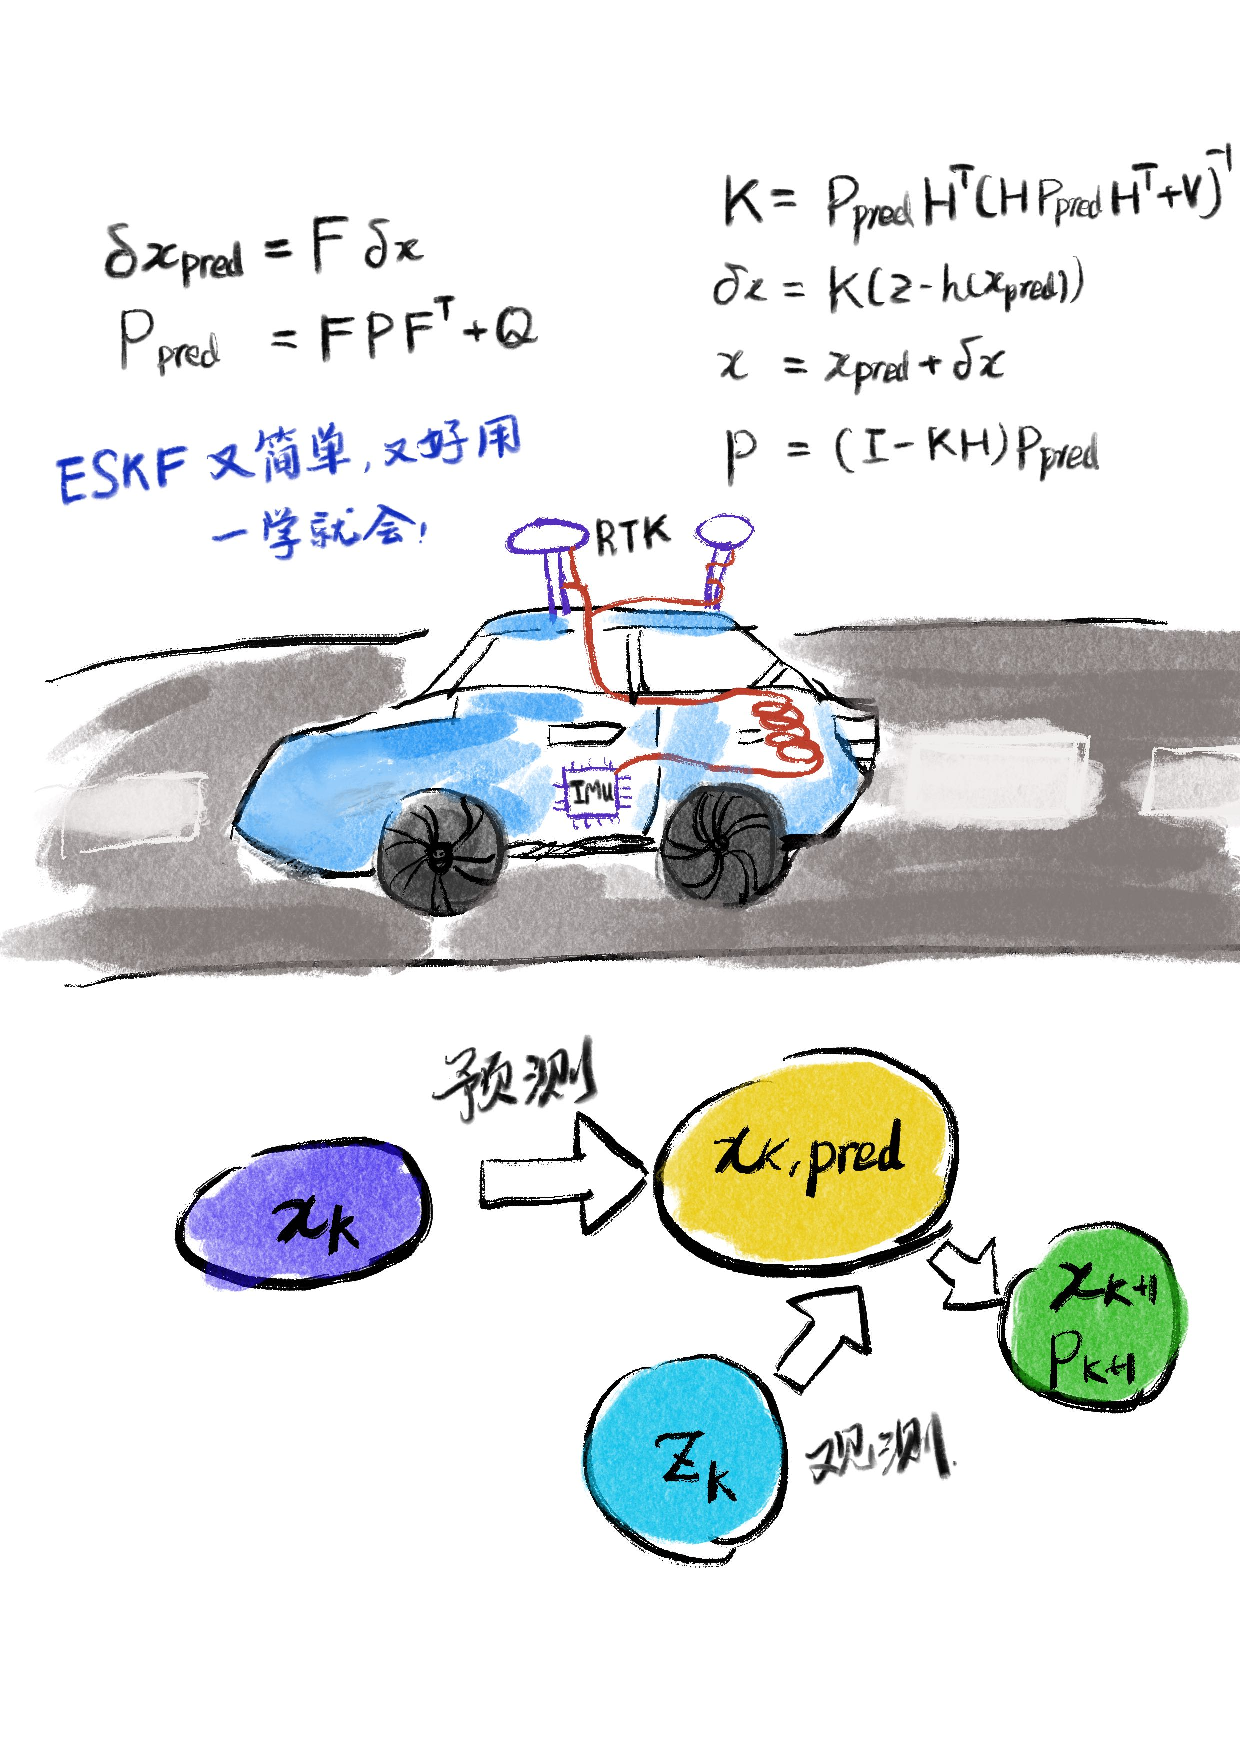
\includepdf[width=\textwidth]{art/ch3.pdf}

\section{Kinematics of IMU Systems}
\label{sec:imu-kinematic}
\subsection{Kinematics}
The \textbf{Inertial Measurement Unit} (IMU) has become very common. IMUs can be found in most electronic devices: vehicles, smartphones, watches, helmets, and even soccer balls. They are small in size and, once installed in a device, can provide effective local motion estimation, enabling various interesting functionalities. In autonomous driving, inertial navigation devices are also fundamental positioning devices. The positioning provided by inertial navigation is basically independent of the external environment and other sensor data, exhibiting high versatility and reliability.

A typical six-axis IMU consists of a \textbf{gyroscope} and an \textbf{accelerometer}. Although they measure the inertia of objects, the means of implementation are diverse, ranging from low-cost MEMS (Micro-electromechanical systems) inertial navigation to expensive fiber-optic gyroscopes (Figure~\ref{fig:real-imus}). Their goal is to accurately measure the inertia of objects. The goal of this book is not to introduce the types and working principles of IMUs themselves\footnote{Readers interested in how IMUs measure angular velocity and acceleration can refer to books that focus more on the manufacturing and measurement principles of IMUs, such as \cite{Qin2014,Yan2019}.}, but to examine their mathematical model properties from the perspective of fusion positioning and state estimation, and further introduce their applications in laser and vision systems.

IMUs are typically installed in a moving system. We infer the state of the object itself by measuring the inertia of the moving carrier. These inertia-related physical quantities are usually not directly position and rotation but rather their differentials. The gyroscope of an IMU can measure the object's \textbf{angular velocity}, while the accelerometer measures the object's \textbf{acceleration}. Internally, they can calculate angular velocity and acceleration based on other physical quantities such as force or time. However, from an external perspective, we only need to be concerned with whether their measurements of angular velocity and acceleration are accurate and the relationship between these quantities and the vehicle's position and orientation.

Based on the kinematics introduced earlier, we can simply write down the kinematic equations in continuous time\footnote{The mathematical symbols in this book are kept simple. We try to avoid adding various subscripts and superscripts, while maintaining consistency throughout the text. However, most of the materials still tend to write out complete symbols with subscripts and superscripts \cite{Huai2018}. This may make the formulae appear more complex, but readers should be able to discern the writing habits of different books.}:

\begin{subequations}\label{eq:motion-equation}
\begin{align}
\dot{\bm{R}} &= \bm{R} \boldsymbol{\omega}^\wedge, \quad \text{or} \  \dot{\bm{q}} = \frac{1}{2} 
\bm{q} \boldsymbol{\omega}, \\
\dot{\bm{p}} &= \bm{v}, \\
\dot{\bm{v}} &= \bm{a}.
\end{align}
\end{subequations}
The rotational part can be represented either by a rotation matrix, as seen in Equation \eqref{eq:rotation-matrix-kinematics}, or by quaternions, as seen in Equation \eqref{eq:quaternion-kinematics}. These physical quantities, when annotated with subscripts, should be denoted as $\bm{R}_{wb}$ and $\bm{p}_{wb}$. Since $\bm{p}_{wb}$ corresponds to the vehicle's world coordinates, after differentiation, it becomes the velocity and acceleration of the vehicle in the world coordinate system, denoted as $\bm{v}_w$ and $\bm{a}_w$. This notation is intuitive, so subsequent text will omit the subscripts related to coordinate systems. Other materials may define variables such as $_w \bm{v}_{wb}$ to distinguish between world-frame velocity and body-frame velocity, but this book uniformly uses quantities in the world frame, with special cases mentioned separately.

The above equations assume that the world frame is fixed, akin to outer space or virtual space. When we do not consider the Earth's rotation, we can simply regard the surface the vehicle travels on as a fixed world coordinate system. In this case, the measured values of IMU, $\tilde{\boldsymbol{\omega}}$ and $\tilde{\bm{a}}$, are the vehicle's own angular velocity and acceleration in the body frame\footnote{We need a notation to distinguish between \textbf{state variables} and \textbf{measurement values}. They can refer to the same physical quantity. However, state variables are estimable and variable, while measurement values are the readings of instruments and are constant. Later text generally uses variables with a tilde to express measurement values, while those without denote state variables.}:
\begin{subequations}\label{key}
	\begin{align}
		\tilde{\bm{a}} &= \bm{R}^\top \bm{a}, \\
		\tilde{\boldsymbol{\omega}} &= \boldsymbol{\omega}.
	\end{align}
\end{subequations}
Note that $\bm{R}^\top$ with the subscript denotes $\bm{R}_{bw}$, which transforms quantities from the world frame to the body frame.

However, real vehicles and robots operate on the surface of the Earth. These systems are influenced by gravity, so we should include gravity in the system equations. In most IMU systems, we can ignore the disturbance caused by the Earth's rotation\footnote{In some high-precision systems, IMUs can measure the Earth's rotation, but in platforms such as vehicles and drones, we usually choose to ignore these physical quantities.}, thus writing the IMU measurements as:
\begin{subequations}\label{eq:3.2}
	\begin{align}
		\tilde{\bm{a}} &= \bm{R}^\top (\bm{a} - \bm{g}), \\
		\tilde{\boldsymbol{\omega}} &= \boldsymbol{\omega}.
	\end{align}
\end{subequations}
Here, $\bm{g}$ represents the gravity of the Earth. Of course, if measuring the object's acceleration in a zero-gravity environment, the gravity term would not appear.

Note that the sign of $\bm{g}$ is related to the definition of the coordinate system. In our coordinate system, both the body frame and the world frame have the $Z$-axis pointing upwards, so $\bm{g}$ typically takes the value $(0, 0, -9.8)^\top$. However, in some books, the $Z$-axis can be defined as pointing towards the center of the Earth, in which case the value of $\bm{g}$ itself or the sign here might be reversed. According to the coordinate system definition in this book, the term in the measurement equation should be $\bm{a}-\bm{g}$.

To aid understanding, readers can also imagine a horizontally placed IMU (see Figure \ref{fig:imu}). If the IMU is stationary, since the measurement of object acceleration is actually obtained by measuring the force applied, the IMU should experience a supporting force in the opposite direction. Therefore, it should measure a gravity in the $-\bm{g}$ direction. If the IMU is flipped upside down, $\bm{R}^\top$ changes, and a positive gravity $\bm{g}$ would be measured. On the other hand, if the IMU is in free fall, the sensors themselves would not detect any external force influence, so $\bm{a}-\bm{g}=\bm{0}$, and the accelerometer should output a zero measurement.

\begin{figure}
	\centering
	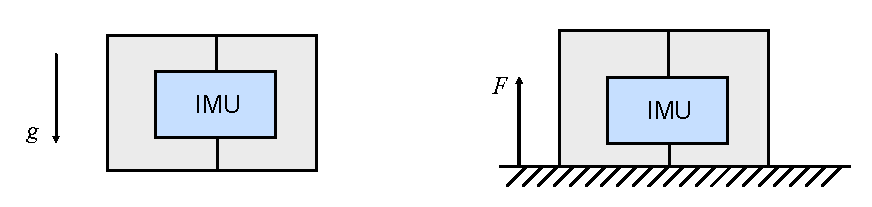
\includegraphics[width=\textwidth]{ins/imu.pdf}
	\caption{Illustration of IMU measurements: during free fall, the IMU does not detect any readings; when horizontally placed, the IMU measures gravity in the opposite direction through the supporting force.}
	\label{fig:imu}
\end{figure}

Note that Equation \eqref{eq:3.2} is written under the assumption of \textbf{no noise influence}. If one wants to design a simulation system, equations without noise models can be used. However, actual IMU measurements typically contain noise, so we need to consider the influence of noise.

\subsection{Explanation of IMU Measurements}

Here, we provide some explanations for the IMU measurement equations mentioned earlier, which might be areas where many students encounter issues in engineering practice.

In theory, according to Newton's second law, the force acting on an object is directly proportional to its acceleration, with the coefficient being the object's mass. For an object located in outer space or in free fall, unaffected by external forces, this is indeed the case. We can also imagine an IMU using springs to measure force. In outer space or during free fall, the springs should be in a relaxed state, and no force should be detected. However, most of the time, we are concerned with real moving objects such as vehicles and robots, which mostly operate on the Earth's surface. Due to the Earth's gravitational force, these objects are naturally subjected to an external force $\bm{g}$. If an object is stationary on the Earth's surface, although the net force acting on it is zero, the IMU still naturally detects a supporting force in the opposite direction. At this time, although the object is not accelerating, the IMU can still read the opposite gravity. Hence, we have a $-\bm{g}$ term in the measurement equation. If we consider an IMU in space, we would remove this gravity term from the measurement equation. Alternatively, if the gravity at a particular location differs from elsewhere, we should adjust the value of $\bm{g}$. However, in some materials, gravity is not included in the measurement equation, and real-world IMUs may remove gravity when outputting data. Readers should be aware of such cases.

Furthermore, if the IMU is not placed at the center of the vehicle, when the vehicle rotates and moves, the IMU should also measure the centrifugal force, Coriolis force, and angular acceleration caused by the vehicle's rotation, reflected in the accelerometer readings. Some vehicles also experience various mechanical vibrations, such as suspension systems, moving parts of the vehicle (brushes, rollers, mechanical arms, etc.), which can also affect IMU readings. Therefore, the complete equation should include these terms. However, if all these small terms are included in the subsequent state estimation equations, the equations will become excessively long, which is not conducive to teaching. In practice, these readings themselves are small, and by ensuring that the IMU is installed as close to the vehicle's center as possible, we can avoid the problems caused by misalignment between the IMU and the vehicle's coordinate system. For these reasons, we will continue to use this simplified IMU measurement model in the subsequent discussions.


\subsection{Noise Model in IMU Measurement Equations}
\label{sec:imu-noise}

In most systems, we consider the noise in an Inertial Measurement Unit (IMU) to consist of two parts: \textbf{measurement noise} and \textbf{bias}. Why do we do this? Due to various reasons, even when a vehicle is stationary, the output of angular velocity and acceleration from an IMU may not form a white noise with a mean of $\bm{0}$, but rather have some \textbf{offset}. This offset is caused by the electromechanical measuring devices within the IMU; some IMUs have small offsets while others may have larger ones. Additionally, this offset is also influenced by factors such as temperature and changes over time. Mathematically, we model it and consider \textbf{bias} as a state variable of the system, which undergoes random changes over time. However, readers should understand that this is a \textbf{mathematical model}, not the \textbf{essence of the system}. We do not derive the variation relationship of bias from the mechanical or physical characteristics of the IMU, nor do we physically describe the relationship between IMU bias and temperature, even if such a relationship objectively exists. We simply \textbf{assume} that the mathematical model is such, and then observe if it significantly differs from the actual readings of the IMU device\footnote{Therefore, readers should not assume that there objectively exists a physically measurable quantity termed bias inside the IMU, and then this quantity is superimposed on the measurement values.}. In most systems, such modeling relationships are sufficient. However, if not, we can also add various compensation parameters as needed to accurately describe the variation of bias.

Let the measurement noise of the gyroscope and accelerometer be denoted as $\boldsymbol{\eta}_g, \boldsymbol{\eta}_a$, and let the biases be denoted as $\bm{b}_g, \bm{b}_a$, where the subscript $g$ represents the gyroscope and $a$ represents the accelerometer. Then, these parameters manifest in the measurement equations as follows:
\begin{subequations}\label{eq:imu-measurement}
	\begin{align}
		\tilde{\bm{a}} &= \bm{R}^\top (\bm{a} - \bm{g}) + \bm{b}_a + \boldsymbol{\eta}_a, \\
		\tilde{\boldsymbol{\omega}} &= \boldsymbol{\omega} + \bm{b}_g + \boldsymbol{\eta}_g.
	\end{align}
\end{subequations}

In continuous time, we consider the IMU measurement noise to be a zero-mean white Gaussian process with variances $\mathrm{Cov}(\boldsymbol{\eta}_g)$ and $\mathrm{Cov}(\boldsymbol{\eta}_a)$\footnote{For basic information on Gaussian processes, readers can refer to Section 2.3 in \cite{Barfoot2016}.}. Additionally, we regard the biases as Wiener processes, also known as Brownian motion or random walk. These are common and classical stochastic processes.

A zero-mean white Gaussian process random variable $\bm{w}(t)$ with covariance $\boldsymbol{\Sigma}$ can be expressed as:
\begin{equation}\label{eq:white-gaussian-process}
	\bm{w}(t) \sim \mathcal{GP}(\bm{0}, \boldsymbol{\Sigma} \delta (t-t')),
\end{equation}
where $\boldsymbol{\Sigma}$ is termed the \textbf{energy spectral density matrix}, and $\delta$ denotes the Dirac delta function. The presence of the Dirac delta function enables us to easily derive the IMU measurement noise after discrete-time sampling from the continuous-time Gaussian process. For detailed derivations, please refer to the appendix of \cite{Crassidis2006}, and we will also discuss this in the subsequent sections when introducing the discrete-time model.

On the other hand, a typical random walk process for a bias $\bm{b}$ can be modeled as:
\begin{equation}\label{eq:random-walk}
	\dot{\bm{b}}(t) = \boldsymbol{\eta}_b (t),
\end{equation}
where $\boldsymbol{\eta}_b (t)$ is also a Gaussian process. Therefore, the random walks for $\bm{b}_a$ and $\bm{b}_g$ can be modeled as follows:
\begin{subequations}\label{eq:bias-random-walk}
	\begin{align}
		\dot{\bm{b}}_a (t) &= \boldsymbol{\eta}_{ba}(t) \sim \mathcal{GP}(\bm{0}, 
		\mathrm{Cov}(\boldsymbol{b}_a) \delta (t-t')), \\
		\dot{\bm{b}}_g (t) &= \boldsymbol{\eta}_{bg}(t) \sim \mathcal{GP}(\bm{0}, 
		\mathrm{Cov}(\boldsymbol{b}_g) \delta (t-t')).
	\end{align}
\end{subequations}

If readers are not familiar with stochastic processes, we can also provide an intuitive understanding. Since the covariance of a Gaussian process increases with time, the measurement values of an IMU itself become less accurate as the sampling time increases. Therefore, a higher sampling frequency IMU tends to have higher precision. Meanwhile, the bias part is described by Brownian motion, exhibiting a random walk behavior. In practice, we can think of an IMU's bias starting from some initial value and randomly moving irregularly around it. The larger the magnitude of this movement, the more unstable the bias is. Therefore, a better quality IMU should maintain its bias near the initial value without significant deviation.

\textbf{Random walk} is essentially a stochastic process whose derivative is a Gaussian process. From the perspective of an IMU, since we are concerned with measuring angular velocity and acceleration, the bias part appears as a random walk. However, from a higher-level system perspective, angular velocity is the derivative of angle, and acceleration is the derivative of velocity. So, the IMU's measurement noise can also be interpreted as a \textbf{random walk of angles} and \textbf{random walk of velocities}. Therefore, when encountering the term "random walk," it's important not to only associate it with the bias part, but rather to consider the problem more holistically.

Please note that Gaussian processes and Brownian motion processes mentioned here are \textbf{mathematical models} of IMU measurement data. Mathematical models do not necessarily correspond exactly to the real world. Sometimes, mathematical models are a \textbf{simplification} of reality, which facilitate subsequent algorithmic computations. We should understand this concept. Later on, when we perform linear approximations and retain various first-order terms in many systems, it's based on this \textbf{simplification} mindset. The real measurement noise and bias of IMUs are influenced by many factors such as vehicle vibration, temperature, IMU's own forces, calibration, installation errors, and so on. Modeling them as two stochastic processes is more for the convenience of state estimation algorithm computation, rather than being a perfect, accurate modeling approach. This \textbf{simplify-then-compensate} approach is very common in practice.

\subsection{Discrete-Time Noise Model for IMU}

Although the noise equations for IMUs in continuous time are relatively complex, they simplify significantly in discrete time. In practice, IMUs sample the inertia of moving objects at fixed time intervals, so the data we obtain is always discrete. The complete derivation of the discrete-time model is cumbersome; interested readers can refer to \cite{Crassidis2006}. Here, we only present the conclusions. Because IMU sensors sample at a fixed frequency, let's assume the sampling interval is $\Delta t$. Then, for the noise, the discrete measurement noises of the gyroscope and accelerometer can be simplified as\footnote{Some small terms from \cite{Crassidis2006} are neglected.}:
\begin{subequations}\label{eq:discrete-noise}
	\begin{align}
		\boldsymbol{\eta}_{g}(k) & \sim \mathcal{N}(0, \frac{1}{\Delta t}  \mathrm{Cov}(\boldsymbol{\eta}_g)),
		\\
		\boldsymbol{\eta}_{a}(k) & \sim \mathcal{N}(0,  \frac{1}{\Delta t} \mathrm{Cov}(\boldsymbol{\eta}_a)) .
	\end{align}
\end{subequations}
As for the bias part, it can be written as:
\begin{subequations}\label{eq:discrete-bias}
	\begin{align}
		\bm{b}_g(k+1) - \bm{b}_g(k) &\sim \mathcal{N}(\bm{0}, \Delta t \ \mathrm{Cov}(\bm{b}_g)), \\
		\bm{b}_a(k+1) - \bm{b}_a(k) &\sim \mathcal{N}(\bm{0}, \Delta t \ \mathrm{Cov}(\bm{b}_a)).
	\end{align}
\end{subequations}

Therefore, in discrete-time systems (which is what we usually deal with), both noises are very easy to handle. In many system implementations, even the \textbf{covariance matrices} are not used to express the IMU measurement noise and bias random walk. Instead, they are simply represented as \textbf{diagonal matrices}, effectively ignoring the correlation between different axes. In programming, parameters such as $\sigma_g, \sigma_a$ are often used to express the \textbf{standard deviations} of IMU noise, and parameters $\sigma_{bg}, \sigma_{ba}$ are used to express the \textbf{standard deviations} of bias drift. In this case, the standard deviations of noise in discrete time should be written as:
\begin{subequations}\label{eq:noise-std-dev}
	\begin{align}
		\sigma_{g}(k) &= \frac{1}{\sqrt{\Delta t}} \sigma_g , \quad	\sigma_{a}(k) = \frac{1}{\sqrt{\Delta t}} 
		\sigma_a, \\
		\sigma_{bg}(k) &= \sqrt{\Delta t} \sigma_{bg} , \quad 	\sigma_{ba}(k) = \sqrt{\Delta t} \sigma_{ba} .
	\end{align}
\end{subequations}
When discussing filters and preintegration later on, we will use these symbols to configure the noise conditions of the IMU. Physically, in discrete time, the noise is directly added to the measured physical quantities, making it easy to determine their physical units. The bias in discrete time itself is added to the measured physical quantities, so they share the same units \cite{Woodman2007}.
\begin{equation}\label{eq:physical-units}
	\sigma_g (k) \rightarrow \frac{rad}{s}, \quad \sigma_a(k) \rightarrow \frac{m}{s^2}, \quad 
	\sigma_{bg}(k) \rightarrow \frac{rad}{s}, \quad \sigma_{ba}(k) \rightarrow \frac{m}{s^2}.
\end{equation}
Continuous-time variances need to be multiplied or divided by a square root time unit to obtain discrete variances, so their physical units become:
\begin{equation}\label{eq:physical-units-continuous}
	\sigma_g  \rightarrow \frac{rad}{\sqrt{s}}, \quad \sigma_a \rightarrow \frac{m}{s \sqrt{s}}, \quad 
	\sigma_{bg} \rightarrow \frac{rad}{s \sqrt{s}}, \quad \sigma_{ba} \rightarrow \frac{m}{s^2 \sqrt{s}}.
\end{equation}
Note that units can be converted between similar units, such as radians to degrees, and seconds to minutes or hours, etc. Some materials may use the unit $\frac{1}{\Delta t}$ as $Hz$, so the physical units of the above variables can also be denoted as:
\begin{equation}\label{eq:physical-units-hertz}
	\sigma_g  \rightarrow \frac{rad}{s \sqrt{Hz}}, \quad \sigma_a \rightarrow \frac{m}{s^2 \sqrt{Hz}}, 
	\quad \sigma_{bg} \rightarrow \frac{rad}{s^2 \sqrt{Hz}}, \quad \sigma_{ba} \rightarrow \frac{m}{s^3 
		\sqrt{Hz}}.
\end{equation}

\subsection{IMUs in Reality}
\begin{figure}
	\centering
	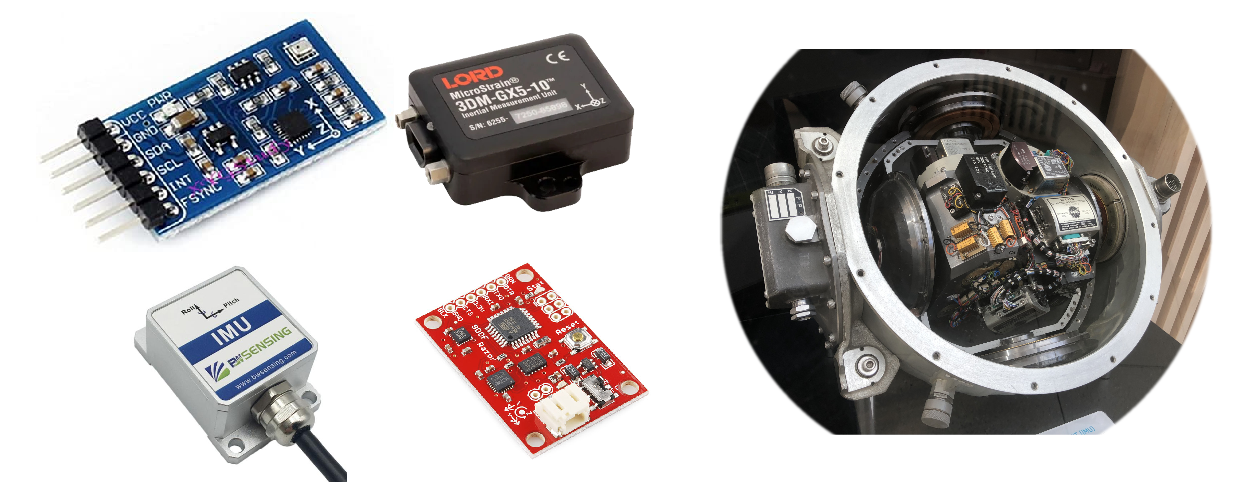
\includegraphics[width=0.9\textwidth]{ins/real-imu.pdf}
	\caption{Various IMU Products in Reality}
	\label{fig:real-imus}
\end{figure}


\begin{figure}
	\centering
	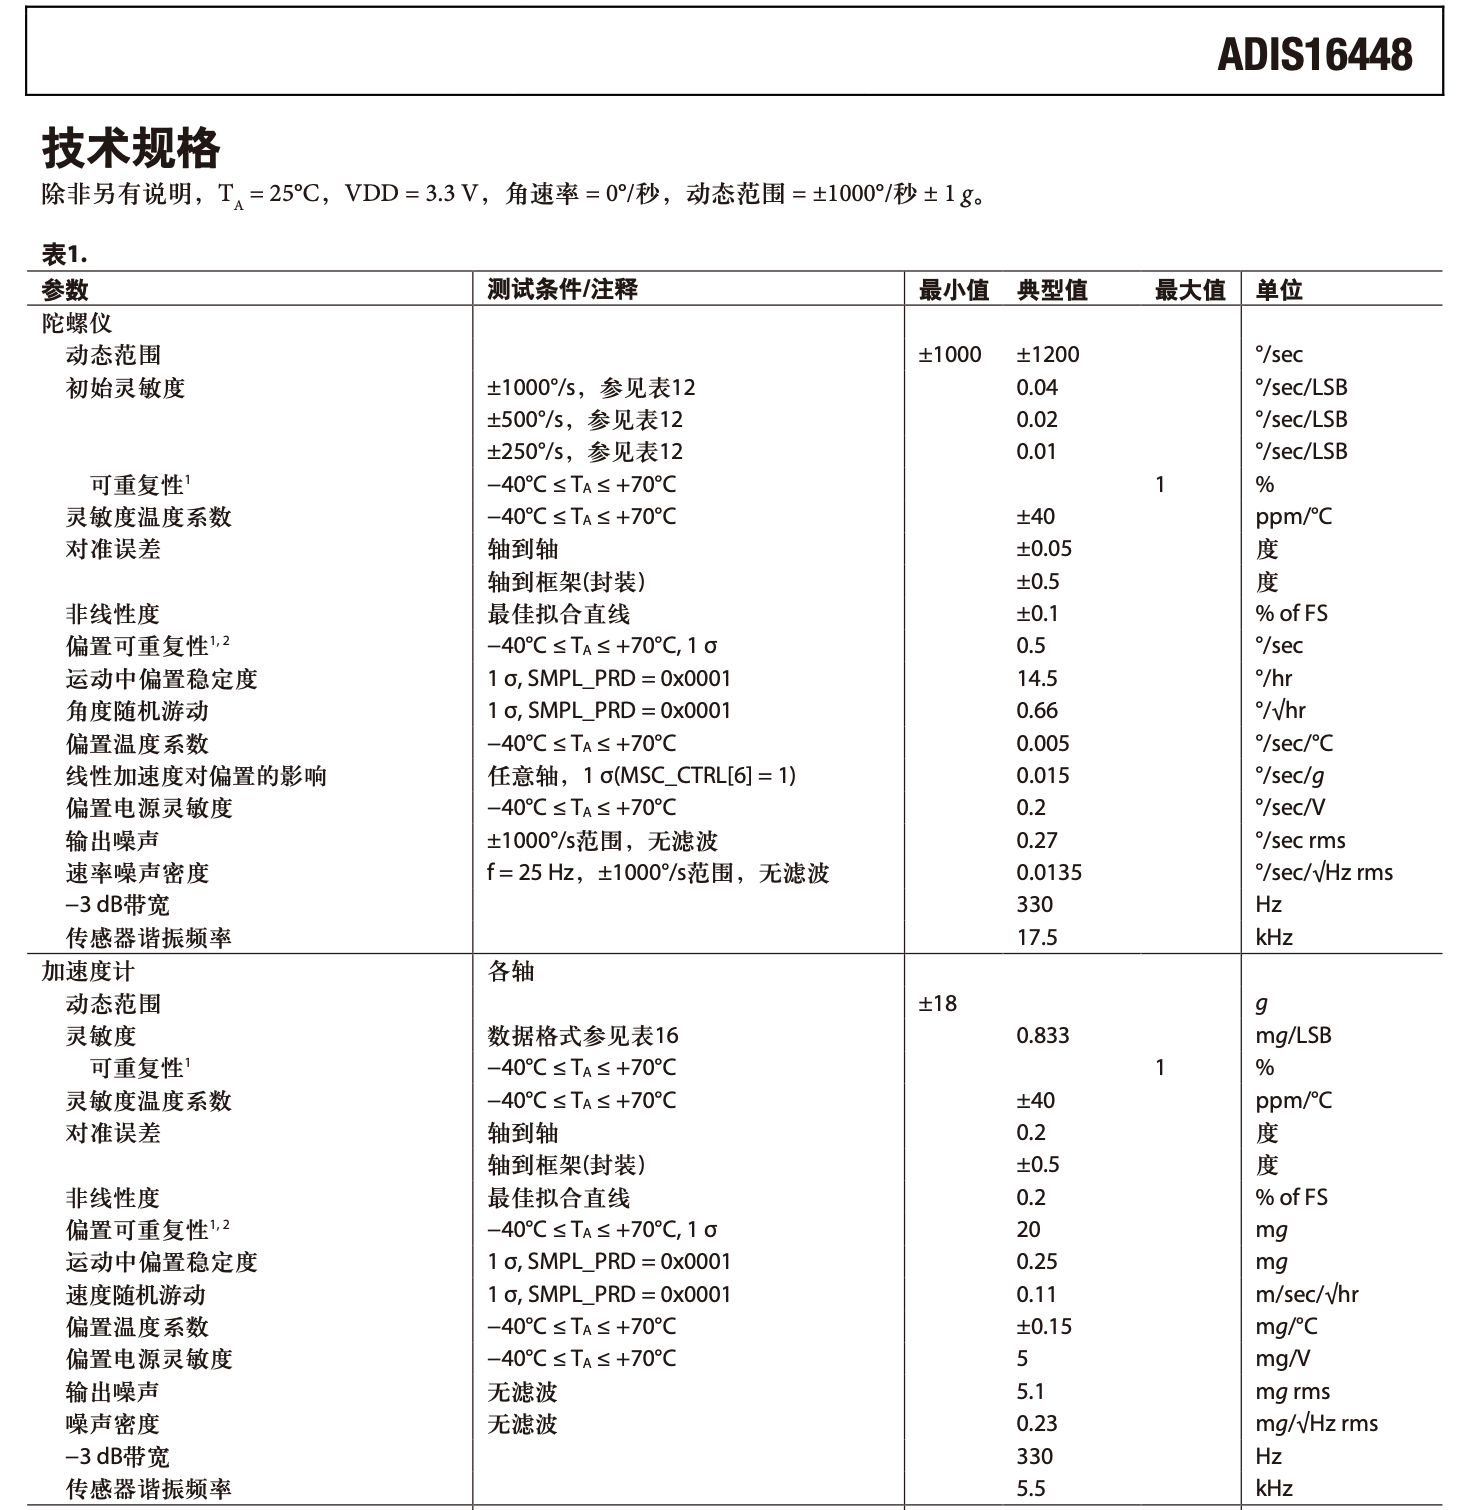
\includegraphics[width=1.0\linewidth]{./ins/imu-datasheet-cn.png}
	\caption{Datasheet of Real IMUs \emph{TODO: replace}}
	\label{fig:imu-datasheet}
\end{figure}

Figure~\ref{fig:real-imus} displays examples of typical IMU products. Readers can directly purchase various IMU-related products in most markets, including standalone IMU sensors and integrated products. With the miniaturization of IMUs, many products are also integrated with IMUs internally at the factory. The most common example is our everyday smartphones, which commonly integrate low-cost MEMS IMU devices. In the field of robotics, sensors commonly used in applications such as LiDAR, cameras, etc., are also increasingly integrating ready-made IMUs. During the period of writing this book, many solid-state LiDARs (e.g., DJI Livox series, Ouster OS2), monocular and stereo cameras (e.g., Zed 2, MYNT Eye S) have already provided built-in IMUs as sources of inertial navigation data.

IMU products generally provide their own datasheets to illustrate their data accuracy, stability, and other metrics at the time of manufacture. These metrics can also be used to guide us in adjusting the weights of state estimation algorithms. Figure~\ref{fig:imu-datasheet} shows a typical parameter configuration of an IMU (ADIS 16488). It can be seen that the main parameters relevant to our subsequent algorithms are as follows:

\begin{enumerate}
	\item Measurement noise, which in the entire motion model is regarded as \textbf{angular random walk} and \textbf{velocity random walk}, corresponding to $\sigma_g$ and $\sigma_a$ in the \textbf{continuous-time} noise model. We can also simply refer to them as \textbf{gyroscope white noise} and \textbf{accelerometer white noise}. It can be observed that the specifications of this IMU are 0.66$^\circ/\sqrt{\text{hour}}$ and 0.11$m/s/\sqrt{\text{hour}}$. Intuitively, this can be understood as follows: assuming we have correctly identified the bias, if we integrate this IMU, the standard deviation of its integration error per hour should be 0.66$^\circ$ and $0.11m/s$.
	
	\item Bias instability variance, which is also known as $\sigma_{bg}$ and $\sigma_{ba}$ in the noise model. However, this quantity is usually not directly corresponding in the datasheet and is difficult to measure in practice. The datasheet often provides bias repeatability and bias stability during operation instead. When we first turn on the IMU, we can estimate the bias of the IMU in a static state. The variability of each bias change is described by bias repeatability. On the other hand, if other objective conditions remain unchanged, this boot-up bias will also change to some extent during operation. Its magnitude is described by \textbf{operational bias stability}, which in this datasheet is 14.5$^\circ /\text{hour}$. Intuitively, under ideal conditions, we can assume that the bias of the IMU will remain within this range near the initial bias. However, in reality, IMUs often do not operate under constant temperature conditions, and their bias changes need to be estimated in real time. Overall, we can refer to this specification to set the magnitude of bias instability.\footnote{For detailed definitions of these two values, please refer to "GJB 585A-1998 Inertial Technology Terminology".}
\end{enumerate}


\section{Trajectory Estimation Using IMU}

Previously, we introduced how angular velocity and acceleration are measured in a motion system. This approach is a simulation-based perspective or a description of a known system. In other words, we can first assume what motion the object undergoes and then consider what kind of IMU measurements should be generated under this motion. However, the reality is the opposite. We can read the readings of IMU sensors, but we must infer the motion of the system based on the readings of IMU and other sensors, rather than directly obtaining various velocity and acceleration information of the system.

When there are many sensors, we integrate various sensor data for fusion-based positioning or SLAM, which is the main content of this book. Later, we will discuss the fusion of IMU with RTK, LiDAR, and other systems. In this section, we will first examine how to infer the motion state of the system when only IMU data is available. We will find that this approach is feasible, but a system with only IMU requires double integration of IMU readings, and the existence of measurement errors and biases will cause the state variables to drift quickly.

\subsection{Short-Term Trajectory Estimation Using IMU Data}

We have introduced the kinematic model of the IMU system itself in Section \ref{sec:imu-kinematic}, while the measurement model of the IMU is introduced in Equation \eqref{eq:imu-measurement}. Therefore, by directly substituting the measurement model into the kinematic equation and ignoring the influence of measurement noise, we can obtain the integration model in continuous time:

\begin{subequations}\label{key}
	\begin{align}
		\dot{\bm{R}} &= \bm{R} (\tilde{\boldsymbol{\omega}} - \bm{b}_g )^\wedge, \quad \text{or} \ 
		\dot{\bm{q}} = \bm{q} \left[0, \frac{1}{2} \left( \tilde{\boldsymbol{\omega}} -\bm{b}_g\right) 
		\right], \\
		\dot{\bm{p}} &= \bm{v}, \\
		\dot{\bm{v}} &= \bm{R} (\tilde{\bm{a}} - \bm{b}_a) + \bm{g}.
	\end{align}
\end{subequations}

Sometimes we also refer to $\bm{p}, \bm{v}, \bm{q}$ as the PVQ state. This equation can be integrated from time $t$ to $t+\Delta t$ to derive the state at the next moment:

\begin{subequations}\label{eq:3.14}
	\begin{align}
		\bm{R}(t+\Delta t) &= \bm{R}(t) \mathrm{Exp} \left( (\tilde{\boldsymbol{\omega}}-\bm{b}_g) \Delta 
		t \right),\quad \text{or} \ \bm{q}(t+\Delta t) = \bm{q}(t) \left[ 1, \frac{1}{2} \left( 
		\tilde{\boldsymbol{\omega}} - \bm{b}_g\right) \Delta t\right], \\
		\bm{p}(t+\Delta t) &= \bm{p}(t) + \bm{v} \Delta t + \frac{1}{2} \left(\bm{R}(t)(\tilde{\bm{a}}-\bm{b}_a) 
		\right) \Delta t^2 + \frac{1}{2} \bm{g} \Delta t^2, \\
		\bm{v}(t+\Delta t) &= \bm{v}(t) + \bm{R}(t) (\tilde{\bm{a}} - \bm{b}_a) \Delta t + \bm{g} \Delta t	.
	\end{align}
\end{subequations}

With this equation, we can use the state at one moment plus the IMU data at the next moment to infer the state at the next moment. This approach is generally referred to as \textbf{recursion}. From the perspective of numerical integration\footnote{Readers unfamiliar with numerical computation can refer to \cite{LiQinYang2001}.}, it corresponds to the Euler method in numerical integration (Figure~\ref{fig:integ-method}).

\begin{figure}
	\centering
	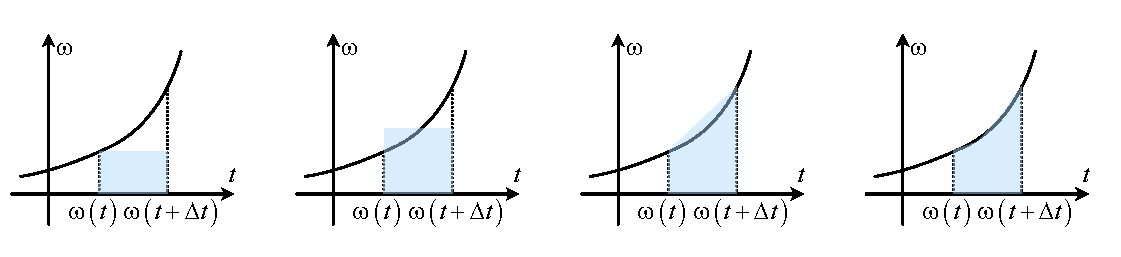
\includegraphics[width=1\textwidth]{ins/integ-method.pdf}
	\caption{Schematic diagram of different integration methods. From left to right: start-point integration, mid-point integration, trapezoidal integration, true integration.}
	\label{fig:integ-method}
\end{figure}

%不同的数值积分方式是不一样的,而欧拉法是最简单的一种。物体本身的旋转和平
%移都是连续的,而IMU则是按照固定时间间隔采样。在采样的这段时间$\Delta t$里,存在若干种不同
%的手段来看待这一小段时间内的角速度与加速度。欧拉法采用了最简单的做法:认为$t$到$t+\Delta t$
%这段时间内,物体整个角速度等于$\boldsymbol{\omega}(t)$,加速度等于$\bm{a}(t)$。这相当于在
%数值积分当中,用小区间的起始点作为积分矩形的函数值。而在另一些做法中,也可以使用中值法、
%梯形法、以及高阶的插值法(最典型的是龙格库塔法\cite{Liu2020})来处理。这些方法在实际当中也
%并不复杂,只需要用插值之后的$\tilde{\boldsymbol{\omega}}, 
%\tilde{\bm{a}}$代替上式当中的观测量,进行递推即可。理论上来讲,中值法、梯形法要比最简单的欧
%拉积分应该更加准确,而插值方法则引入了额外的计算量,其精度提升相比计算量的提升是否值得,
%要视具体应用而定。
%
%上式也可以进一步累积,比如从$i$时刻一直递推到$j$时刻。我们只需把中间的IMU读数累计起来即
%可:
%\begin{subequations}\label{eq:imu-dead-reckoning}
%\begin{align}
%\bm{R}_j &= \bm{R}_i \prod_{k=i}^{j-1}\mathrm{Exp} \left(\left(\tilde{\boldsymbol{\omega}}_k - 
%\bm{b}_{g,k}\right) \Delta t\right) \quad \text{或}\ \bm{q}_j = \bm{q}_i \prod_{k=i}^{j-1} \left[1, 
%\frac{1}{2} \left(\tilde{\boldsymbol{\omega}}_k - \bm{b}_{g,k}\right) \Delta t \right], \\
%\bm{p}_j &= \bm{p}_k + \sum_{k=i}^{j-1} \left[\bm{v}_k \Delta t + \frac{1}{2} \bm{g} \Delta t^2\right] + 
%\frac{1}{2} \sum_{k=i}^{j-1} \bm{R}_k \left(\tilde{\bm{a}}_k - \bm{b}_{a,k} \right) \Delta t^2, \\
%\bm{v}_j &= \bm{v}_i + \sum_{k=i}^{j-1}\left[ \bm{R}_k\left(\tilde{\bm{a}}_k - \bm{b}_{a,k} \right) 
%\Delta t+ \bm{g} \Delta t  \right].
%\end{align}
%\end{subequations}
%
%注意我们这里还没有考虑噪声的影响。在第~\ref{cpt:preinteg}~讲中,我们将进一步考察测量噪声和零偏噪声对IMU积分之后的影响,这里我们只看它的递推形式。注意到上式实际上是\textbf{增量形式}的,每一个$\bm{R}_k, \bm{v}_k$都可以作为计算结果,用到下一个时刻中。所以在代码实现中,在某帧IMU到达后,我们可以用上一帧的结果来计算下一帧的递推结果,而不必等待所有数据到达后再按照公式进行累加。在旋转方面,使用四元数还是旋转矩阵,并没有本质差别,不过旋转矩阵的表示在数学公式上会更加简洁一些,而且不用经常归一化。本章我们仍然保留两种写法,以供读者随时对比。但在后续章节中,我们将主要使用旋转矩阵的表达方式。
%
%\subsection{IMU递推的代码实验}
%下面我们通过一个实验来看看如何用IMU数据进行轨迹的推算。在没有外部观测时,我们只能用式(\ref{eq:imu-dead-reckoning})
%来进行二次积分,得到运动物体本身的位置和姿态信息。这种积分通常是快速发散的,因此IMU并不
%适合单独拿来进行航迹推算。我们的实验也将展现这一点。
%
%\begin{lstlisting}[language=c++,caption=ch3/imu\_integration.h]
%class IMUIntegration {
%	public:
%	IMUIntegration(const Vec3d& gravity, const Vec3d& init_bg, const Vec3d& init_ba)
%	: gravity_(gravity), bg_(init_bg), ba_(init_ba) {}
%	
%	// 增加imu读数
%	void AddIMU(const IMU& imu) {
%		double dt = imu.timestamp_ - timestamp_;
%		if (dt > 0 && dt < 0.1) {
%			// 假设IMU时间间隔在0至0.1以内
%			p_ = p_ + v_ * dt + 0.5 * gravity_ * dt * dt + 0.5 * (R_ * (imu.acce_ - ba_)) * dt * dt;
%			v_ = v_ + R_ * (imu.acce_ - ba_) * dt + gravity_ * dt;
%			R_ = R_ * Sophus::SO3d::exp((imu.gyro_ - bg_) * dt);
%		}
%		
%		// 更新时间
%		timestamp_ = imu.timestamp_;
%	}
%	
%	/// 组成NavState
%	NavStated GetNavState() const { return NavStated(timestamp_, R_, p_, v_, bg_, ba_); }
%	
%	SO3 GetR() const { return R_; }
%	Vec3d GetV() const { return v_; }
%	Vec3d GetP() const { return p_; }
%	
%	private:
%	// 累计量
%	SO3 R_;
%	Vec3d v_ = Vec3d::Zero();
%	Vec3d p_ = Vec3d::Zero();
%	
%	double timestamp_ = 0.0;
%	
%	// 零偏,由外部设定
%	Vec3d bg_ = Vec3d::Zero();
%	Vec3d ba_ = Vec3d::Zero();
%	
%	Vec3d gravity_ = Vec3d(0, 0, -9.8);  // 重力
%};
%\end{lstlisting}
%
%该函数实现了简单的IMU积分器,可以持续读取IMU数据,并给出自身的积分结果。我们在data/ch3/
%中给读者准备了一些传感器数据(在后续章节还会用到)。读者可以任选一段轨迹,运行以下程序,
%查看IMU积分的结果。
%\begin{lstlisting}[language=c++,caption=ch3/run\_imu\_integration.cc]
%sad::TxtIO io(FLAGS_imu_txt_path);
%
%// 该实验中,我们假设零偏已知
%Vec3d gravity(0, 0, -9.8);  // 重力方向
%Vec3d init_bg(00.000224886, -7.61038e-05, -0.000742259);
%Vec3d init_ba(-0.165205, 0.0926887, 0.0058049);
%
%sad::IMUIntegration imu_integ(gravity, init_bg, init_ba);
%
%sad::ui::PangolinWindow ui;
%ui.Init();
%
%/// 记录结果
%auto save_result = [](std::ofstream& fout, double timestamp, const Sophus::SO3d& R, const Vec3d& v,
%const Vec3d& p) {
%	auto save_vec3 = [](std::ofstream& fout, const Vec3d& v) { fout << v[0] << " " << v[1] << " " << v[2] << " "; };
%	auto save_quat = [](std::ofstream& fout, const Quatd& q) {
%		fout << q.w() << " " << q.x() << " " << q.y() << " " << q.z() << " ";
%	};
%	
%	fout << std::setprecision(18) << timestamp << " " << std::setprecision(9);
%	save_vec3(fout, p);
%	save_quat(fout, R.unit_quaternion());
%	save_vec3(fout, v);
%	fout << std::endl;
%};
%
%std::ofstream fout("./data/ch3/state.txt");
%io.SetIMUProcessFunc([&imu_integ, &save_result, &fout, &ui](const sad::IMU& imu) {
%	imu_integ.AddIMU(imu);
%	save_result(fout, imu.timestamp_, imu_integ.GetR(), imu_integ.GetV(), imu_integ.GetP());
%	ui.UpdateNavState(imu_integ.GetNavState());
%	usleep(1e2);
%}).Go();
%
%ui.Quit();
%\end{lstlisting}
%
%该程序会把积分结果存储在ch3/state.txt中。注意本书会大量使用C++中的lambda函数来实现灵活的函数调用。这里的TxtIO负责读取文本文件并解析传感器数据,然后按照预设的回调函数来执行各种传感器的回调。由于不同章节的程序需要将这些传感器数据进行不同的处理,这里的回调部分以lambda函数实现。
%
%现在来执行这个程序:
%\begin{lstlisting}[language=sh, caption=终端输入:]
%bin/run_imu_integration
%\end{lstlisting}
%
%它会在UI中显示车辆实时位置。不过这个程序会很快发散,车辆会消失在屏幕边缘。在程序结束之后,我们运行绘图脚本就可以绘制这段轨迹:
%\begin{lstlisting}[language=sh, caption=终端输入:]
% python3 scripts/plot_ch3_state.py data/ch3/state.txt 
%\end{lstlisting}
%
%\begin{figure}
%	\centering
%	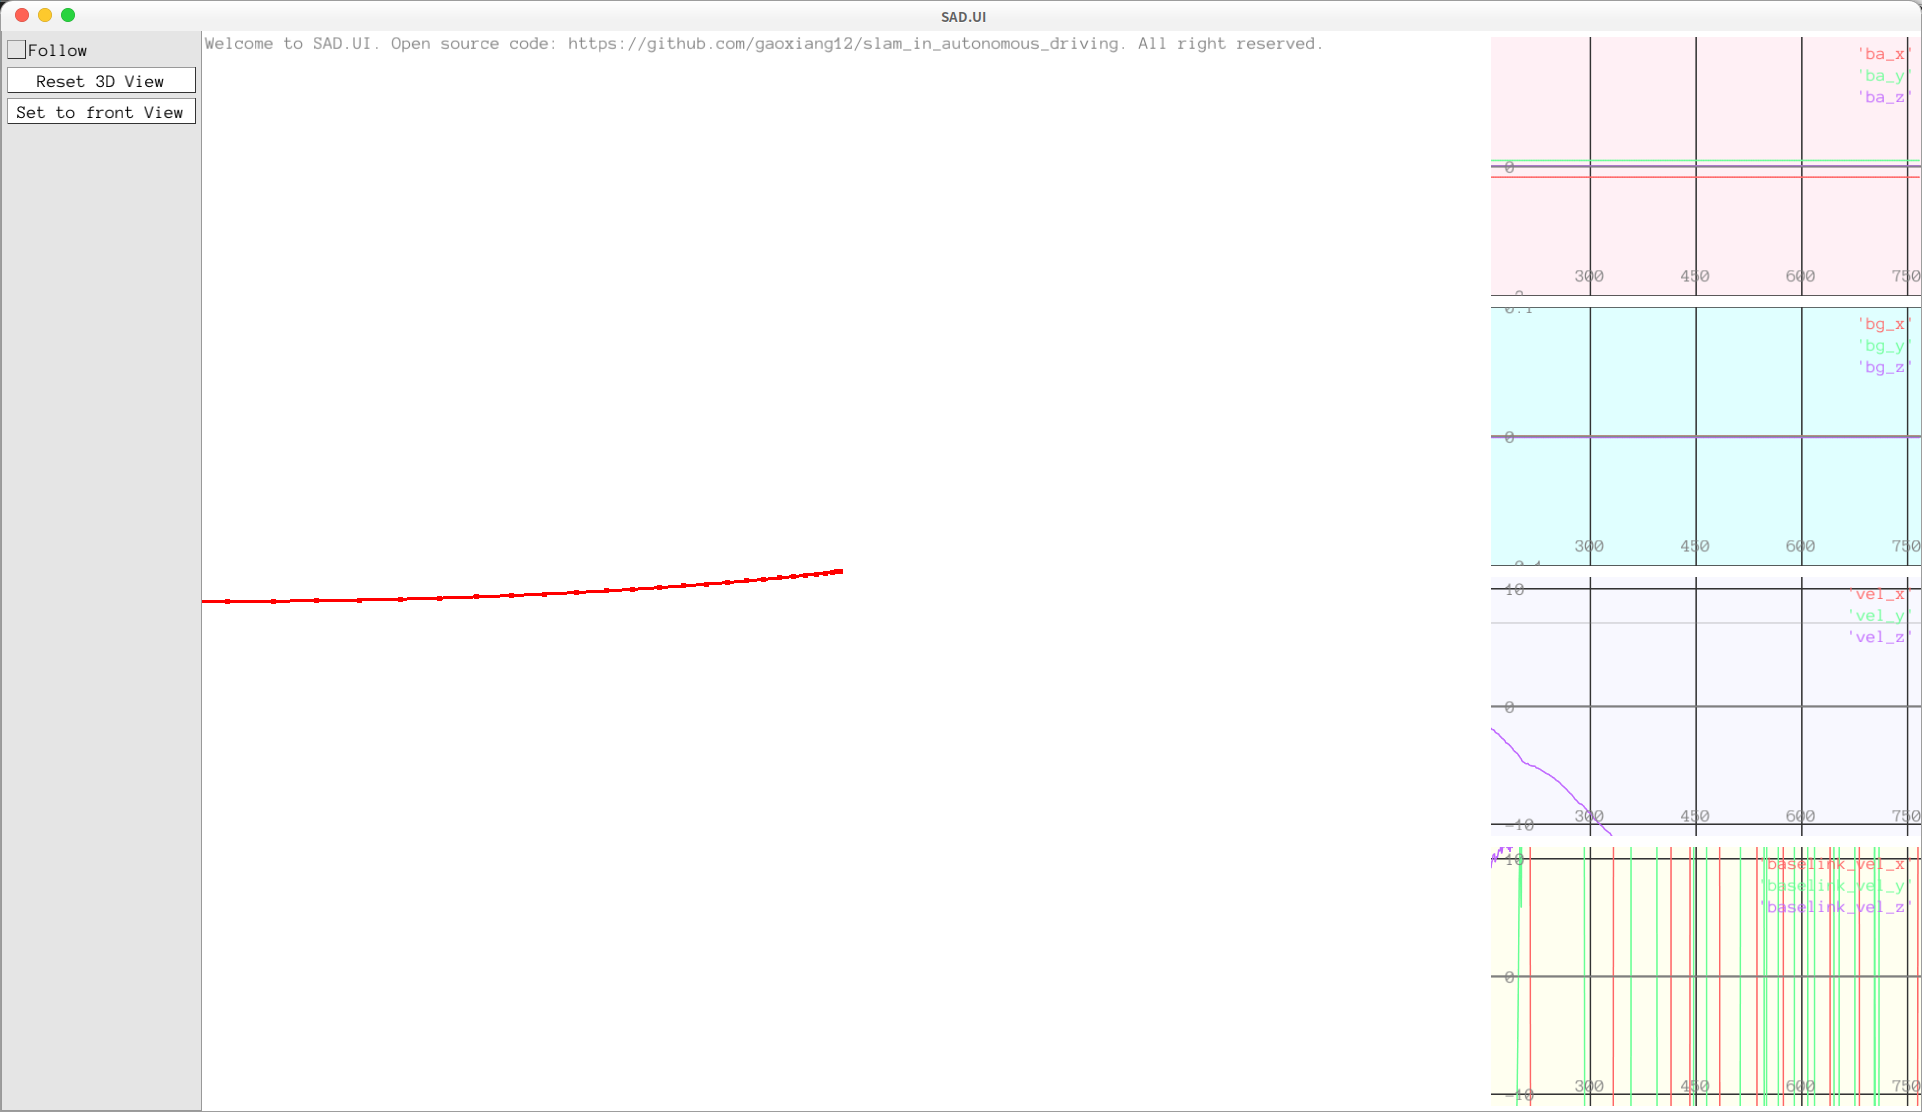
\includegraphics[width=1\textwidth]{ins/ch3-imu-integ-ui.png}
%	\caption{IMU积分结果在UI中显示}
%	\label{fig:ch3-imu-integ-ui}
%\end{figure}
%
%UI里的车辆运动如图~\ref{fig:ch3-imu-integ-ui}所示,轨迹的绘制结果如图~\ref{fig:ch3-imu-integ}~所示。我们看到,以四元数表达的姿态整体上仍能保持稳定。该数据来源是车载IMU,四元数姿态中的$q_y, q_z$一直保持在零附近,但位移方面则很快发散。由于缺少外部观测,速度状态很快超出了控制,远远大于车辆的实际速度(该车辆为时速低于25公里的低速车辆),使得位置估计发散到一个很大的数值。读者也可以尝试其他数据,它们都会快速发散。
%
%\begin{figure}
%	\centering
% 	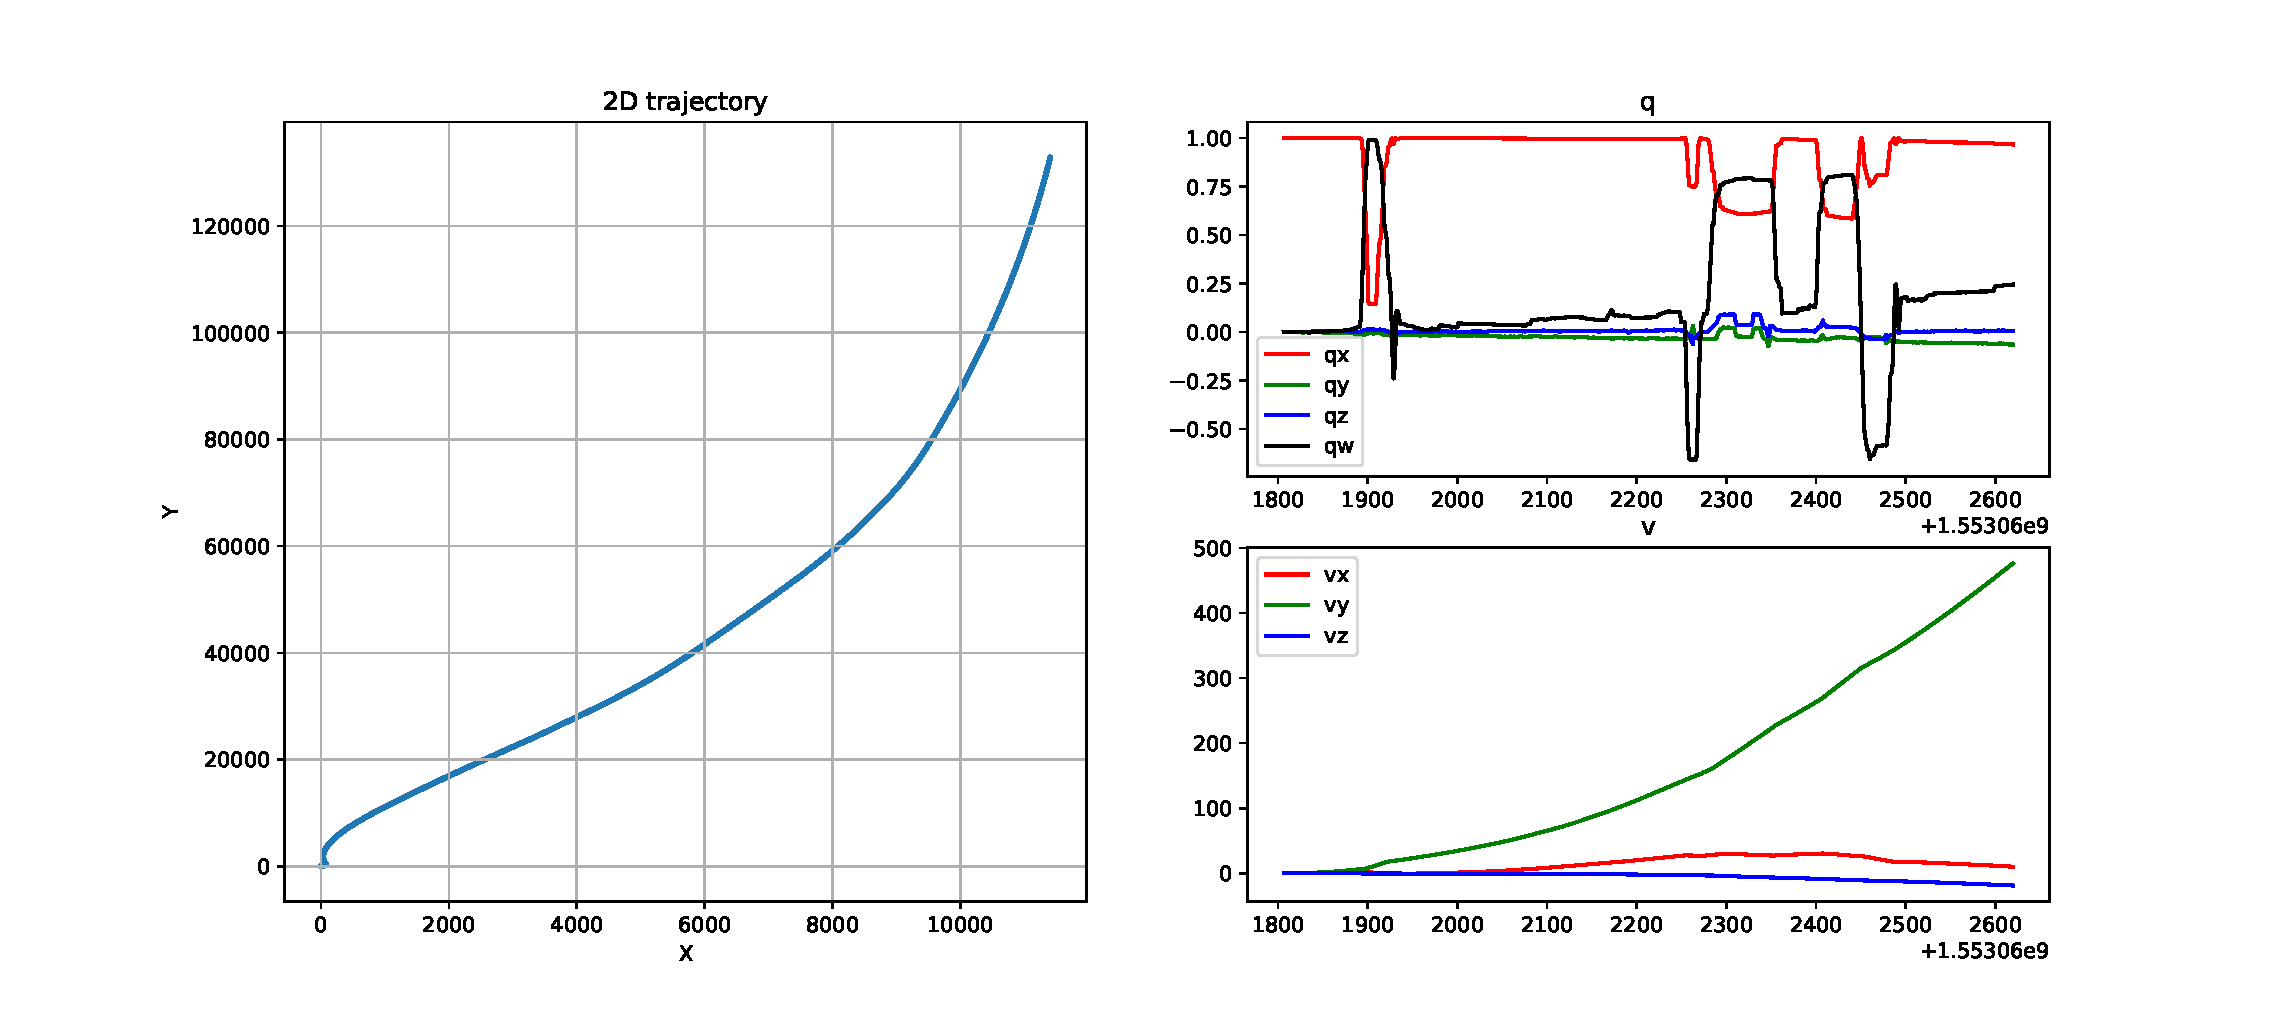
\includegraphics[width=1\textwidth]{ins/ch3-imu-integ.pdf}
%	\caption{IMU积分的结果}
%	\label{fig:ch3-imu-integ}
%\end{figure}
%
%后面我们将介绍如何将其他传感器数据与IMU进行融合,来得到更准确的状态估计。在传统导航领域,IMU最主要的融合方式是和卫星导航进行组合,这样的系统称为GINS(GNSS-INS)系统。
%
%\section{卫星导航}
%卫星导航(Global Navigation Satellite System, GNSS)是室外车辆定位的另一个主要信息来源。卫星导航内部原理非常复杂,然而它的输出结果却十分简单。当然从某种角度来说,如果把实用的系统拆分到原理层面,人们很快就会被工程细节淹没。即使像单片机这样看起来简单的系统,如果从
%电路层面讲起,也会显得十分复杂。所以,我们并不准备从如何发射火箭或卫星开始介绍GNSS系统,
%而是从另一个更加实际的角度来看这个问题,那就是,从自动驾驶车辆的视角来看,卫星导航
%能给一辆车提供什么信息?
%
%这个问题的答案倒是十分简单的。在正常工作的时候,卫星导航实际上可以提供车辆所需的\textbf{所
%有定位信息},包括车辆的位置、姿态、速度等物理量。于是读者会问,那是否只靠卫星定位都可以
%实现自动驾驶呢?要回答这个问题,我们需要考量几个方面的因素:
%
%\begin{enumerate}
%	\item GNSS提供的定位精度是否满足要求?
%	\item GNSS的定位频率是否足够下游使用?
%	\item GNSS的定位可用性如何?是否能够全天候全场地使用?
%\end{enumerate}
%
%实际上,GNSS也存在许多个细分种类,对上述问题的答案也并没有统一的回答。有些GNSS定位方
%法可以提供很高精度,但必须要求物体静止一段时间(通常十分钟以上);也有的方法可以提供较好
%的动态物体定位,但需要事先架设一个或多个基站。几乎所有GNSS都存在“看天吃饭”的问题——它
%们的稳定性与场景、结构、物体的遮挡关系、甚至和当天的天气有关。这使得在自动驾驶行业中,卫星导航大多数时候处于
%一种精度够用,但稳定性很难控制的状态。
%
%\subsection{GNSS的分类与供应商}
%% GNSS接收器图
%整体而言,GNSS系统通过测量自身与地球周围各卫星的距离来确定自身的位置,而与卫星的距离主
%要是通过测量时间间隔来确定的。一个卫星信号从卫星上发出时,带有一个发送时间。而GNSS接收机接收到它时,又有一个接收时间。我们比较接收时间与卫星发送时间,就能估算各卫星离我们的距离。而各种GNSS系统和测量方法的主要差异,就是如何减少这个时间的误差。从这种角度来看,GNSS本质上可以看成一种高精度的授时系统。
%
%\begin{figure}
%	\centering
%	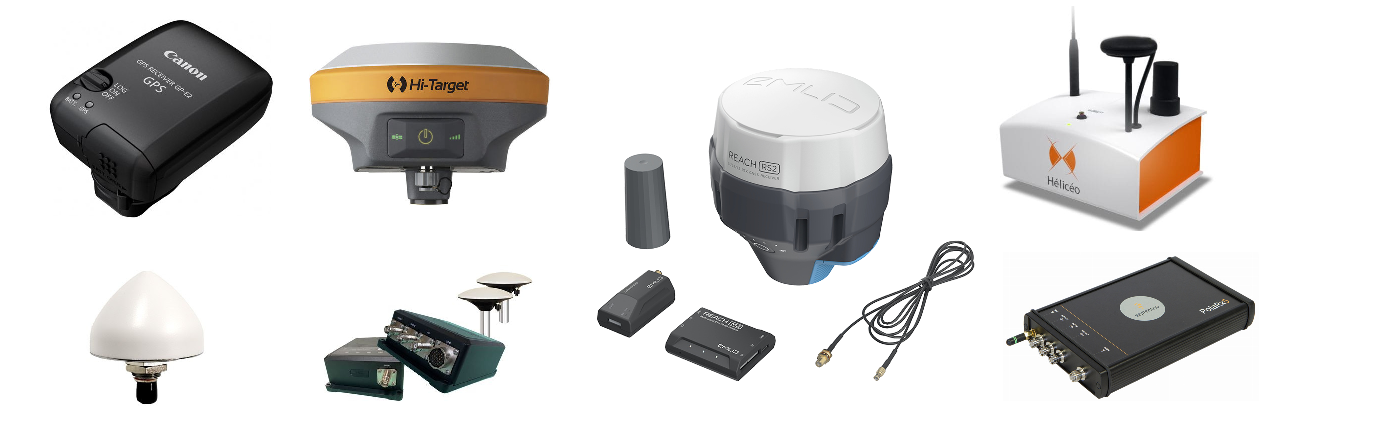
\includegraphics[width=0.7\textwidth]{ins/rtk-receivers.pdf}
%	\caption{各式各样的GNSS/RTK接收机。}
%	\label{fig:rtk-receivers}
%\end{figure}
%
%目前世界范围内,我们可以接收到卫星信号主要来自四个系统:美国的全球定位系统(Global 
%Positioning System, GPS)、中国的北斗卫星导航系统(Beidou Navigation Satellite System, 
%BDS)、俄罗斯的格洛纳斯系统(GLONASS)、欧盟的伽利略系统(GALILEO)。每个系统都在空
%间中部署了20至30颗卫星。直接利用这些卫星定位信息的系统通常称为\textbf{单点GNSS}定位\footnote{GNSS
%系统一直在发展,出于一些历史原因,早期的人们习惯于使用GPS这个称呼,但现在大部分文献会区
%分GPS和GNSS的名词。}。大部分位于地面的GNSS接收机都可以接收到各卫星系统的信号。
%它们可以选择其中一个卫星定位信息来源,也可以同时使用多个卫星信号来源。
%这种单点GNSS定位系统通常能够提供数米范围内的定位精度。大部分手机设备上就使用单点GNSS进行定位和导航(图~\ref{fig:rtk-receivers})。
%
%卫星定位的最终精度受很多因素影响。从发射端的卫星电磁信号,到中间的传输过程,再到接收端的
%时钟信号,每一种误差都可能引起最终卫星定位的结果偏差。同时,人们也提出了各种各样的校正技
%术来消除这些已知的误差。近几年人们发展了\textbf{PPP}(Precise Point 
%Positioning,精密单点定位)、\textbf{RTK}(Real-Time 
%Kinematic,实时动态差分)等技术,其定位精度仍在不断提升。实际上这些技术的涵盖面非常广泛,本书在从使用人员而非研发人员的角度来看待
%问题,故不针对各种卫星定位的改进技术作深入论述。感兴趣的读者请参考\cite{李晓欢2020, 
%周建华2020}等文献。在2023年的今天,GNSS定位已经从早年的10米左右的定位精度,逐渐提升到实
%时可用的厘米级别定位精度,而且已经可以面向大众。截止到目前,国内的GNSS服务商也越来越
%丰富,千寻、合众、讯腾等公司已能提供覆盖广泛、价格合理的卫星定位服务。这些终端也逐渐走进
%消费者的手机、汽车等产品内部。
%
%对于自动驾驶汽车来说,最常用的卫星定位技术包括以下几种:
%\begin{enumerate}
%	\item 单点GNSS定位,即传统的米级精度卫星定位。这种定位方式价格低廉,应用广泛。大多数
%	手机、车机等终端都具备单点卫星定位能力。在普通车辆的道路级导航当中\footnote{自动驾驶通常需要\textbf{
%	车道级}导航而非\textbf{道路级}导航。车道级导航可以指出车辆位于道路当中哪个车道,比道路级
%	导航要更稳定一些。},单点定位的精足以让驾驶人员辩认出车辆位于哪条道路,但在多条道路并排时,它的精度又往往不足以区分车辆是在高速路上还是辅路上,或者在主路还是匝道的情况。
%	\item 
%	RTK定位。由于卫星定位信号在传输过程中可能产生误差,人们发展了\textbf{差分定位技术},即
%	通过地面上的一个已知精确位置的基准站与车辆通讯,校正车辆卫星接收机的信号。差分定位又可
%	进一步分为位置、伪距以及载波相位差分定位。其中最广泛使用的,是基于\textbf{载波相位差分}的RTK技
%	术。RTK通过与一个或多个基站进行通信,可以实时地获取校正后的卫星导航位置。
%\end{enumerate}
%
%目前已有多家企业为自动驾驶提供RTK服务。这些企业通常会大范围地架设基准站,通过4G和5G移动网络与
%车辆进行实时通信,输出车辆的实时位置。在天气、路况较好的场景,我们可以直接使用RTK提供的
%定位信息来实现自动驾驶。也有一些供应商组合RTK与惯导系统,构成更加稳定的组合导航算法,从而增
%加定位系统的可靠性。
%
%\subsection{实际的RTK安装与接收数据}
%百闻不如一见。下面我们向读者展示一些自动驾驶中实际接收的RTK数据(GNSS数据同理)。RTK接收器通常安装在车
%辆顶部,呈圆盘形状(人们通常亲切地称为“蘑菇头”)。一个蘑菇头可以提供精确卫星定位位置,如
%果使用两个接收器组成\textbf{双天线}方案,那就可以根据两根天线给出的位置差,计算车辆的实时
%朝向(heading)。
%
%\begin{figure}
%	\centering
%	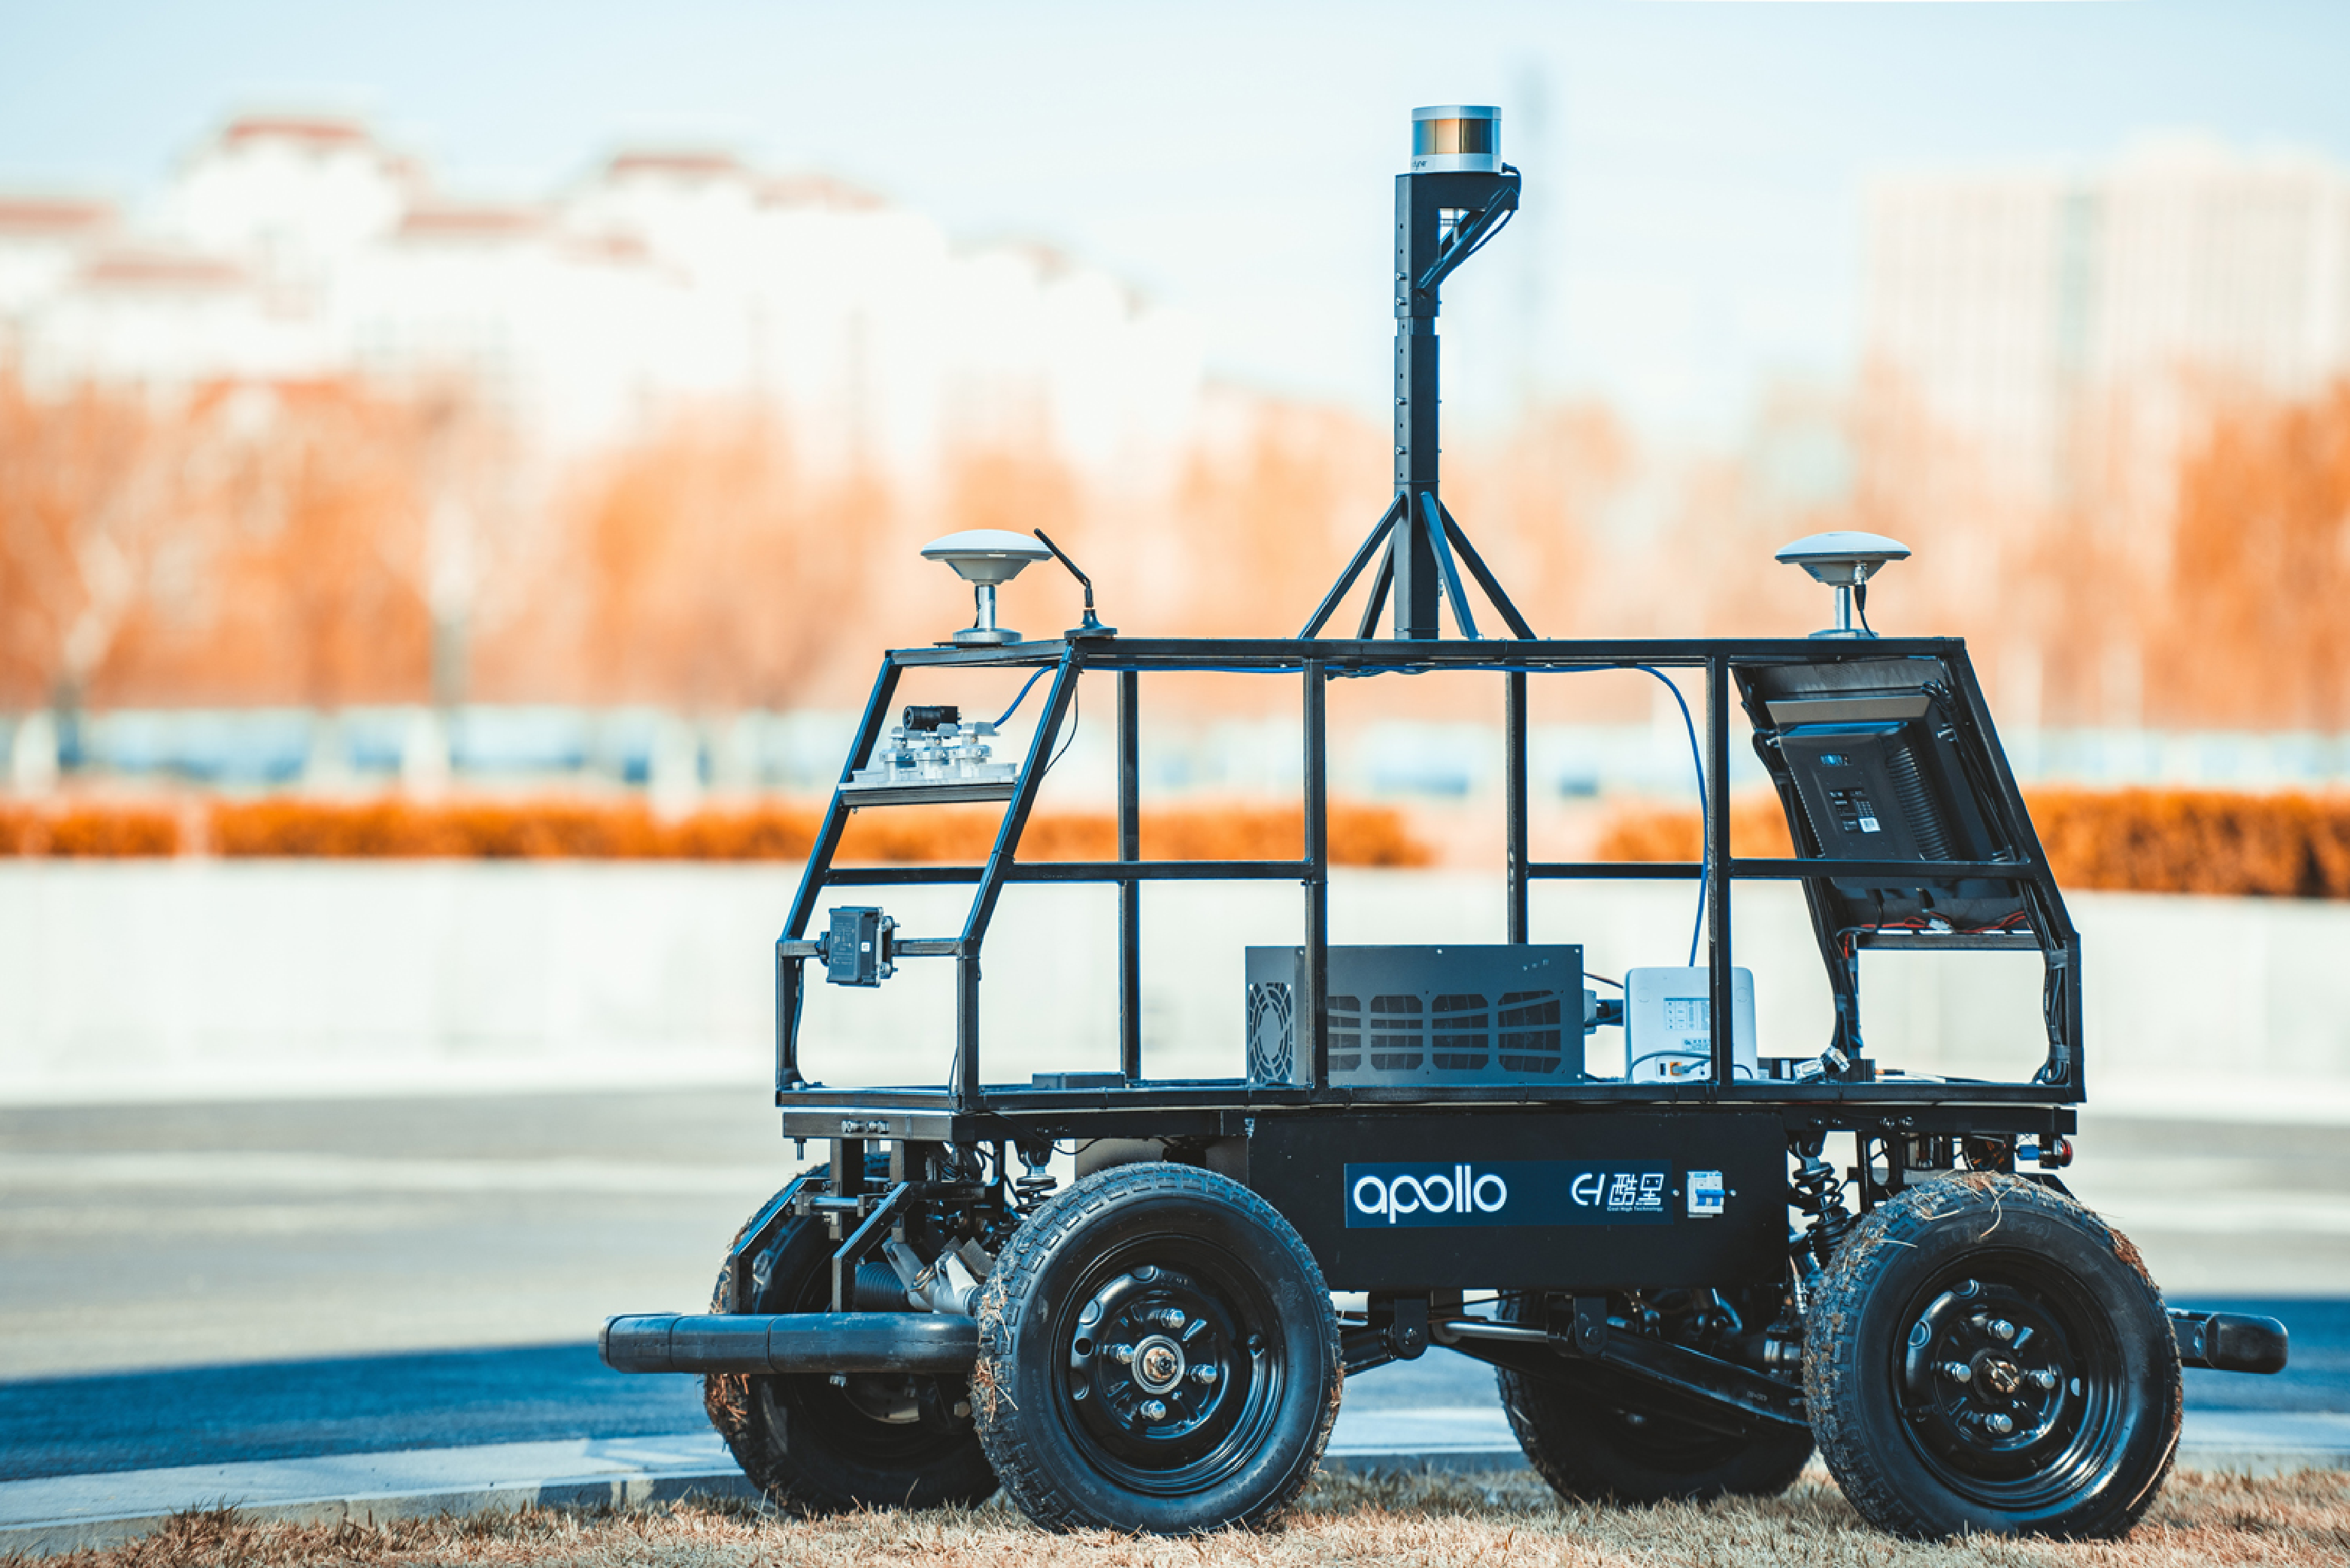
\includegraphics[width=0.7\textwidth]{ins/apollo-rtk.pdf}
%	\caption{百度阿波罗开发套件的一种RTK天线安装方式。}
%	\label{fig:apollo-rtk}
%\end{figure}
%
%图~\ref{fig:apollo-rtk}~展示了一种实际车辆上的RTK双天线方案。这个车辆没有外壳,我们容易从照片中看出来各类传感
%器的安装位置。这台车辆有两个RTK蘑菇头,一个在车辆前方,另一个在车辆后方,它们是沿着车辆前进轴放置的。
%也有些车辆的双天线采用水平安装或者侧向安装方法。总体而言,双天线方案中,我们定义其中一个为主天线,表达车辆位置。然后以另一个为副天线,将主副天
%线的位置矢量相减,得到两根天线之间的朝向,进而获取车辆角度(主要为航向角yaw)。在左右安装的方案中,通常以左侧为
%主天线; 而在前后安装方案中,通常以后侧为主天线。不过,这些只是人为定义,两根天线没有什
%么本质上的不同,反着定义也是完全可以的。
%
%图~\ref{fig:rtk-antenna}~展示了几种RTK天线的不同安装方式,实际当中也可以按照车辆本身外形进
%行定制。为了准确测量车辆角度,人们往往会把两根天线放得尽可能远\footnote{两根天线的位置都会
%受一定噪声的影响。当它们的距离越远时,测量噪声对角度的影响就会变小。}。双天线的距离也叫
%做RTK的\textbf{基线}(baseline)\footnote{基线这个词定义非常广泛,各种传感器都可以有将自己某条线段定义为基线,比如RTK的基线、双目视觉的基线,等等。读者不必纠结这个词与其他地方所说的基线之间的联系。}。RTK本身作为一种传感器,在车辆上的安装位置可以视为它的外
%参,可以由一个矩阵描述。不过,由于双天线一般在一个水平面内,它的旋转部分外参只需用一个角
%来描述,称为\textbf{安装偏角}(antenna angle);平移部分则称为\textbf{安装偏移}(antenna 
%position)。这两个参数一般在结构设计时确定。
%
%\begin{figure}
%	\centering
%	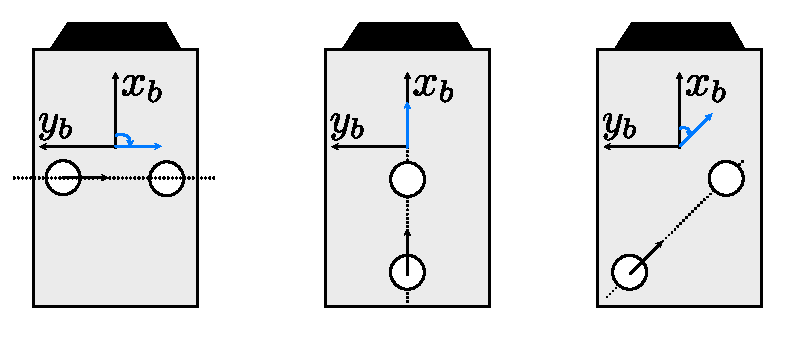
\includegraphics[width=0.7\textwidth]{ins/rtk-antenna.pdf}
%	\caption{RTK双天线的不同安装方式:左右安装、前后安装、对角安装。}
%	\label{fig:rtk-antenna}
%\end{figure}
%
%卫星定位普遍输出物体的经纬度位置。这种输出形式与地球上某个固定的坐标系相关,而不像其他激光、视觉定位那样可以随意定义坐标系。同时,双天线RTK的角度也存在习惯的定义方式。我们先来介绍常见的世界坐标系,再来处理一些实际的RTK数据。
%
%\subsection{常见的世界坐标系}
%物理世界当中存在多种普遍使用的世界坐标系。我们来简单介绍一下它们的定义方式。
%
%\subsubsection{地理坐标系}
%\begin{figure}
%	\centering
%	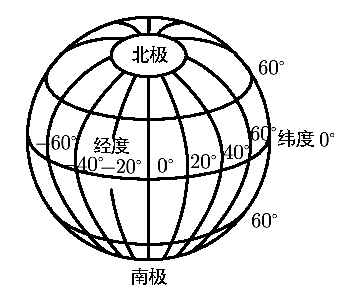
\includegraphics[width=0.4\textwidth]{ins/latlon.pdf}
%	\caption{经纬度坐标系示意图}
%	\label{fig:latlon}
%\end{figure}
%
%地球上最常见的坐标系就是\textbf{经纬度}(latitude longitude)坐标系,也称为\textbf{地理坐标系}(Geographic Coordinate System),参见图~\ref{fig:latlon}。它们再加上高度就形成了经纬高坐标系(latitude-longitude-altitude, LLA)。经纬度是指按横向和纵向对地球表面进行均匀的切分。经度从本初子午线向东西各180度,纬度则是从赤道向南北各90度。这两个数值均为角度值或者弧度值。高度方面则可使用海拔高度或者地心高度,它们都是相对于某个基准水平面的高度。
%
%经纬度是十分直观、好用的坐标系,能够覆盖整个地球。许多地图系统都会首选使用经纬度坐标作为默认的坐标系。但自动驾驶地图通常在城市级别或者更小的范围内,经纬度坐标会让坐标系统有效数字变多(建筑物级别的经纬度通常要精确到小数点后8至9位),读起来比较费力。它们与日常接触的米制单位转换关系也不够线性,例如一度经度在北极可以对应0米,而在赤道可能对应上百公里。因此,除了经纬度这种全局坐标系,我们还会使用一些日常的局部坐标系。
%
%\subsubsection{UTM坐标系}
%%\begin{figure}
%%	\centering
%%	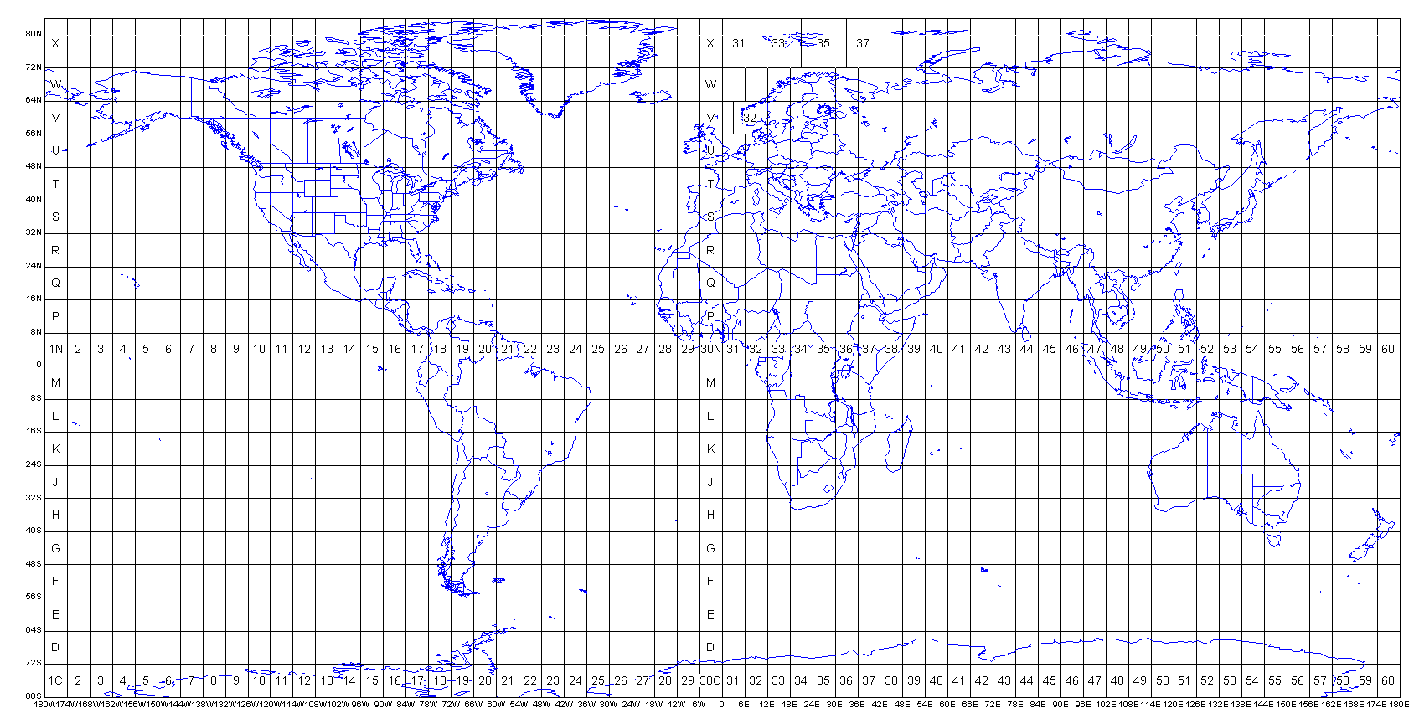
\includegraphics[width=1.0\textwidth]{ins/utm.pdf}
%%	\caption{UTM坐标系的分区示意图}
%%	\label{fig:utm}
%%\end{figure}
%
%UTM(Universal Transverse Mercator Grid System)坐标系是将地球视为一个椭球体(World Geodetic System 84椭球体),投影至横躺的圆柱体上,然后展开进行分区后得到的。它将经度分为60个区,将纬度分为20个区,并赋予标号。经度方向为数字标号,纬度方向为字母标号。除个别地方外,这些分区大体是均匀分布的。注意这里所谓的均匀分布是指沿经纬度均匀分布,但由于地球本身是球面,它们在米制单位上并不是均匀的。另外,两极区域在铺平之后有较大畸变,所以UTM的纬度有效范围是南北80度以内。
%
%在每个分区内,UTM坐标以正东,正北的米制坐标来表达车辆位置。由于地球半径约6378公里,可以算得UTM一格在东西向最宽约66.7万米。于是,UTM正东坐标是指,将该区的经度中心线取为$x=500000$,然后取向东的偏移量。此时,如果某个点落在中心线以西,则$x$坐标将小于500000米,但仍为正数。正北方向则以赤道的投影距离为原点,取这个点偏离赤道的距离为$y$坐标。那么,在北半球中,我们将正东视为$X$轴,正北视为$Y$轴,按照右手坐标系,$Z$轴应该指向天空。这样就定义了一个分区内的世界坐标系,且符合\textbf{东北天坐标系}习惯。或者,也可以正北为$X$轴,以正东为$Y$轴,$Z$轴指向地面,定义\textbf{北东地坐标系}。两者在实际应用中都有使用。
%
%UTM的优点是使了米制坐标,与其他传感器的兼容性好,缺点是某些地区可能在两个分区的跨界处,需要额外的坐标处理。由于地球的投影畸变,实际的UTM坐标与米制单位之间还有一个0.9996的倍数关系,在高精度场合中需要考虑进去。此外,\textbf{东北天坐标}与\textbf{北东地坐标}的$Z$轴指向相反,所以在角度定义方面会有差别,这在实际情况中也应该进行转换。
%
%\subsection{RTK读数的显示}
%不少RTK和组合导航生产厂商都可以按照用户选择的坐标系往外输出坐标,其中最基本的就是输出RTK接收器测量到的经纬度。下面我们演示如何将RTK的经纬度坐标转换为米制的UTM坐标,同时使用双天线方案确定车辆的方向角。这里我们不考虑车辆的俯仰和滚转,把它们视为零。于是,虽然车辆输出的是\textbf{四自由度坐标},但在假设车辆俯仰和滚转为零的前提下,也可以把RTK输出视为六自由度的位置变换,即$\mathrm{SE}(3)$的位姿。
%
%我们继续使用上一节的数据。这些数据实际上是IMU、RTK、轮速计读数的数据文件,位于data/ch3/下。读者可以用文本编辑器打开它们,格式如下:
%
%\begin{lstlisting}[language=sh, caption=数据文件例子]
%GNSS 1571900872.47168827 30.0011840411666668 117.97859182983332 305.98748779296875 
%330.047799999999995 1
%ODOM 1571900872.50085688 0 0
%IMU 1571900872.56527948 -0.000740019602845583204 -0.000471238898038460995 
%6.98131700797720067e-06 0.362519161666666645 -0.0608012299999999908 
%9.82135997500000002
%\end{lstlisting}
%文件的每一行表示一个数据,开头的“GNSS”、“IMU”、“ODOM”表达它的记录类型。对于GNSS读数
%来说,每行的内容为:记录时间、纬度、经度、高度、方向角、方向角有效位标志。对于IMU或轮速
%来说,则是各自的加速度计、陀螺仪和轮速计的读数。这里的GNSS定位是由千寻FindCM方案提供
%的,在固定解状态下标称精度为2cm。
%
%由于经纬度转UTM的算法比较复杂和琐碎,不是本书的重点内容,我们使用一个开源的转换方法来实
%现这部分内容,参见thirdparty/utm\_convert目录\footnote{工具地址见:\url{https://github.com/hobu/mgrs}}。我们为它添加一个封装函数,让我们方便
%地计算GNSS读数对应的$\mathrm{SE}(3)$位姿。转换代码如下:
%
%\begin{lstlisting}[language=c++,caption=ch3/utm\_convert.cc]
%bool LatLon2UTM(const Vec2d& latlon, UTMCoordinate& utm_coor) {
%	long zone = 0;
%	char char_north = 0;
%	long ret = Convert_Geodetic_To_UTM(latlon[0] * math::kDEG2RAD, latlon[1] * math::kDEG2RAD, &zone, &char_north,
%	&utm_coor.xy_[0], &utm_coor.xy_[1]);
%	utm_coor.zone_ = (int)zone;
%	utm_coor.north_ = char_north == 'N';
%	
%	return ret == 0;
%}
%
%bool ConvertGps2UTM(GNSS& gps_msg, const Vec2d& antenna_pos, const double& antenna_angle, const Vec3d& map_origin) {
%	/// 经纬高转换为UTM
%	UTMCoordinate utm_rtk;
%	if (!LatLon2UTM(gps_msg.lat_lon_alt_.head<2>(), utm_rtk)) {
%		return false;
%	}
%	utm_rtk.z_ = gps_msg.lat_lon_alt_[2];
%	
%	/// GPS heading 转成弧度
%	double heading = 0;
%	if (gps_msg.heading_valid_) {
%		heading = (90 - gps_msg.heading_) * math::kDEG2RAD;  // 北东地转到东北天
%	}
%	
%	/// TWG 转到 TWB
%	SE3 TBG(SO3::rotZ(antenna_angle * math::kDEG2RAD), Vec3d(antenna_pos[0], antenna_pos[1], 0));
%	SE3 TGB = TBG.inverse();
%	
%	/// 若指明地图原点,则减去地图原点
%	double x = utm_rtk.xy_[0] - map_origin[0];
%	double y = utm_rtk.xy_[1] - map_origin[1];
%	double z = utm_rtk.z_ - map_origin[2];
%	SE3 TWG(SO3::rotZ(heading), Vec3d(x, y, z));
%	SE3 TWB = TWG * TGB;
%	
%	gps_msg.utm_valid_ = true;
%	gps_msg.utm_.xy_[0] = TWB.translation().x();
%	gps_msg.utm_.xy_[1] = TWB.translation().y();
%	gps_msg.utm_.z_ = TWB.translation().z();
%	
%	if (gps_msg.heading_valid_) {
%		// 组装为带旋转的位姿
%		gps_msg.utm_pose_ = TWB;
%	} else {
%		// 组装为仅有平移的SE3
%		// 注意当安装偏移存在时,并不能实际推出车辆位姿
%		gps_msg.utm_pose_ = SE3(SO3(), TWB.translation());
%	}
%	
%	return true;
%}
%\end{lstlisting}
%
%其中经纬度到UTM的转换由库函数完成,而我们需要把GNSS坐标系下的UTM坐标转换为车辆的观测位姿,其中要考虑RTK的安装外参。本节使用的双天线RTK安装方式如图~\ref{fig:dual-rtk-coor}~所示,蓝色的$x_B, y_B, O_B$表示车身坐标系,红色的$x_G, y_G, O_G$表示GNSS接收器的坐标系。
%
%数学上,可以将RTK的UTM坐标读数视为$\bm{T}_{WG}$,其中$W$代表世界坐标系,$G$代表GNSS
%接收器的坐标系。为了方便后续的融合定位,我们将它转换到$\bm{T}_{WB}$,其中$B$为车辆本体
%坐标系。于是GNSS接收器与车辆间的外参就可以由$\bm{T}_{GB}$或$\bm{T}_{BG}$描述。
%
%\begin{figure}
%	\centering
%	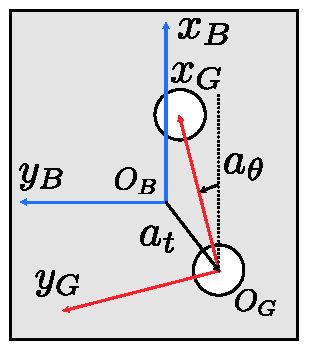
\includegraphics[width=0.3\textwidth]{ins/dual-rtk-coor.pdf}
%	\caption{本书样例中使用的RTK安装方式。下标$G$表示GNSS接收器的坐标系,$B$表示车辆本体坐标系。这台车辆的主天线位于车辆右后侧,副天线位于左前侧。}
%	\label{fig:dual-rtk-coor}
%\end{figure}
%
%在标定参数中,我们指定安装偏移$\bm{a}_t$为$O_B$指向$O_G$的矢量,且在$B$系中取坐标,这实际上就是$\bm{T}_{BG}$的平移分量。同
%时,安装偏角$a_{\theta}$定义为$B$系的$x$轴转向$G$系$x$轴之间的转角。将$\bm{a}_t, a_{\theta}$代入到$\bm{T}_{BG}$中,不难得到:
%\begin{equation}\label{key}
%	\bm{T}_{BG} = \begin{bmatrix}
%		\bm{R}_Z (a_{\theta}) &  \bm{a}_t \\
%		\bm{0}^\top & 1
%	\end{bmatrix},
%\end{equation}
%其中$\bm{R}_Z$表示绕$Z$轴进行旋转的矩阵。
%
%需要解释的是,这种\textbf{安装偏角}和\textbf{安装偏移}的定义方式是符合直观的,但它并不是唯一的,具体定义方式需要照顾到操作上的便利性。这两个量也可以按照反方向来定义,只要现场标定人员可以很容易地测量出来。我们往往让数学符号习惯跟从现实习惯,而不是让现实操作来符合数学定义。如果我们让标定人员测量$\bm{R}_{BG}$或者$\bm{t}_{BG}$,他往往无法很直观地想象出来。但我们给出两个点的连线,或者两条线的夹角,人们就很容易操作。
%
%车辆本体系到世界系的变换矩阵$\bm{T}_{WB}$可由RTK读数和它的外参解出:
%\begin{equation}\label{key}
%\bm{T}_{WB} = \bm{T}_{WG} \bm{T}_{GB}.
%\end{equation}
%
%将此式的旋转与平移部分写开,可得:
%\begin{equation}\label{key}
%\bm{R}_{WB} = \bm{R}_{WG} \bm{R}_{GB}, \quad \bm{t}_{WB} = \bm{R}_{WG} \bm{t}_{GB} + \bm{t}_{WG}.
%\end{equation}
%
%这里要提一点,即使RTK外参$\bm{t}_{GB}$已知,要确定车辆坐标$\bm{t}_{WB}$,还需要知道RTK的朝向$\bm{R}_{WG}$。如果我们使用的是单天线方案,而安装偏移相关的量$\bm{t}_{GB}$又不为零,那么\textbf{当车辆朝向不明时,并不能真正确定车辆本体的世界坐标}。当然,在状态估计算法中,车辆姿态$\bm{R}_{WB}$存在估计值,此时也可以使用$\bm{R}_{WB} \bm{R}_{BG}$来作为当时的$\bm{R}_{WG}$。
%
%此外,这里的转换程序还做了\textbf{东北天}至\textbf{北东地}的转换。由于RTK生产厂商的协议并不相同,有些厂商在输出角度时会按照他们预定的方案来实现,这可能会导致角度定义的不一致。本书使用的UTM坐标使用正东正北作为$XY$轴,属于\textbf{东北天}坐标系;而RTK厂商输出的则是\textbf{北东地}坐标系。前者以东为零度,后者以北为零度,且旋转方向相反。于是一个北东地坐标系下的方位角$h$转换到东北天坐标系下的角度$h'$,应为:
%\begin{equation}\label{key}
%h' = \pi/2 - h.
%\end{equation}
%上述代码就对方位角作了上述处理。
%
%接着,我们再写一段程序,将数据文件中的GNSS读数转换为位姿后,写入输出的文件。读者可
%以用python脚本绘制整个GNSS的轨迹。同时我们也把RTK的位姿放入实时图形界面中,让读者可以马上看到当前的位置和朝向。
%
%\begin{lstlisting}[language=c++,caption=ch3/process\_gnss.cc]
%DEFINE_string(txt_path, "./data/ch3/10.txt", "数据文件路径");
%
%// 以下参数仅针对本书提供的数据
%DEFINE_double(antenna_angle, 12.06, "RTK天线安装偏角(角度)");
%DEFINE_double(antenna_pox_x, -0.17, "RTK天线安装偏移X");
%DEFINE_double(antenna_pox_y, -0.20, "RTK天线安装偏移Y");
%
%/**
%* 本程序演示如何处理GNSS数据
%* 我们将GNSS原始读数处理成能够进行后续处理的6自由度Pose
%* 需要处理UTM转换、RTK天线外参、坐标系转换三个步骤
%*
%* 我们将结果保存在文件中,然后用python脚本进行可视化
%*/
%
%int main(int argc, char** argv) {
%	sad::TxtIO io(fLS::FLAGS_txt_path);
%	
%	std::ofstream fout("./data/ch3/gnss_output.txt");
%	Vec2d antenna_pos(FLAGS_antenna_pox_x, FLAGS_antenna_pox_y);
%	
%	auto save_result = [](std::ofstream& fout, double timestamp, const SE3& pose) {
%		auto save_vec3 = [](std::ofstream& fout, const Vec3d& v) { fout << v[0] << " " << v[1] << " " << v[2] << " "; };
%		auto save_quat = [](std::ofstream& fout, const Quatd& q) {
%			fout << q.w() << " " << q.x() << " " << q.y() << " " << q.z() << " ";
%		};
%		
%		fout << std::setprecision(18) << timestamp << " " << std::setprecision(9);
%		save_vec3(fout, pose.translation());
%		save_quat(fout, pose.unit_quaternion());
%		fout << std::endl;
%	};
%	
%	std::shared_ptr<sad::ui::PangolinWindow> ui = nullptr;
%	if (FLAGS_with_ui) {
%		ui = std::make_shared<sad::ui::PangolinWindow>();
%		ui->Init();
%	}
%	
%	bool first_gnss_set = false;
%	Vec3d origin = Vec3d::Zero();
%	io.SetGNSSProcessFunc([&](const sad::GNSS& gnss) {
%		sad::GNSS gnss_out = gnss;
%		if (sad::ConvertGps2UTM(gnss_out, antenna_pos, FLAGS_antenna_angle)) {
%			if (first_gnss_set == false) {
%				origin = gnss_out.utm_pose_.translation();
%				first_gnss_set = true;
%			}
%			gnss_out.utm_pose_.translation() -= origin;
%			
%			save_result(fout, gnss_out.unix_time_, gnss_out.utm_pose_);
%			ui->UpdateNavState(
%				sad::NavStated(gnss_out.unix_time_, gnss_out.utm_pose_.so3(), gnss_out.utm_pose_.translation()));
%			
%			usleep(1e4);
%		}
%	}).Go();
%	
%	if (ui) {
%		while (!ui->ShouldQuit()) {
%			usleep(1e5);
%		}
%		ui->Quit();
%	}
%	
%	return 0;
%}
%\end{lstlisting}
%
%该程序将RTK读数转换为UTM位姿,并去除了原点,然后写入文本文件,同时传递给UI进行显示。请读者编译运行该程序,指定一个输入的文本文件:
%\begin{lstlisting}[language=sh, caption=终端输入:]
%bin/process_gnss --txt_path ./data/ch3/10.txt
%\end{lstlisting}
%
%该程序将RTK转换后的六自由度坐标写入data/ch3/gnss\_output.txt文件中。接下来我们可以用scripts/plot\_ch3\_gnss\_2d和3d两种脚本分别绘制二维和三维的GNSS轨迹:
%\begin{lstlisting}[language=sh, caption=终端输入:]
%python3 scripts/plot_ch3_gnss_2d.py ./data/ch3/gnss_output.txt 
%\end{lstlisting}
%
%二维和三维的轨迹图如图~\ref{fig:gnss-traj}~所示。可见,这个场景中RTK本身能够给出非常不错的车辆轨迹,但高度层面则存在明显抖动和误差,
%说明RTK的高度测量数据精度通常是不如水平坐标的。读者也可以尝试画出本书提供的其他几个样例
%数据,只需更改对应的文件路径即可。此处展示的案例是一个GNSS信号良好的场景,不过我们提供
%的数据里也存在一些GNSS相对较差的路段,读者可以对比一下它们的轨迹图。
%
%\begin{figure}
%	\centering
%	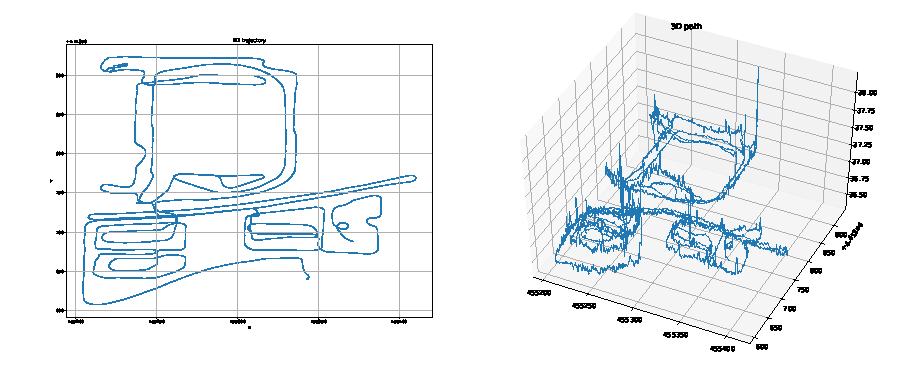
\includegraphics[width=1.0\textwidth]{ins/gnss-traj.pdf}
%	\caption{GNSS轨迹的二维和三维视图。}
%	\label{fig:gnss-traj}
%\end{figure}
%
%本节测试程序也会提供实时的GNSS位姿展示,如图~\ref{fig:process-gnss}。在RTK角度有效时,车辆应该为$X$轴向前,$Y$轴向左,$Z$轴向上。如果读者自己运行了本程序,应该能观察到RTK测量的角度相比位置更加不稳定一些。在运行过程中,RTK角度经常会出现失效的情况。而按照我们之前的推导,如果RTK姿态失效,车辆本身的位置也将无法完全解算出来。所以读者还应该能观察到,在RTK角度失效时,我们计算出来的车辆位置也会有小幅度的抖动。
%
%\begin{figure}
%	\centering
%	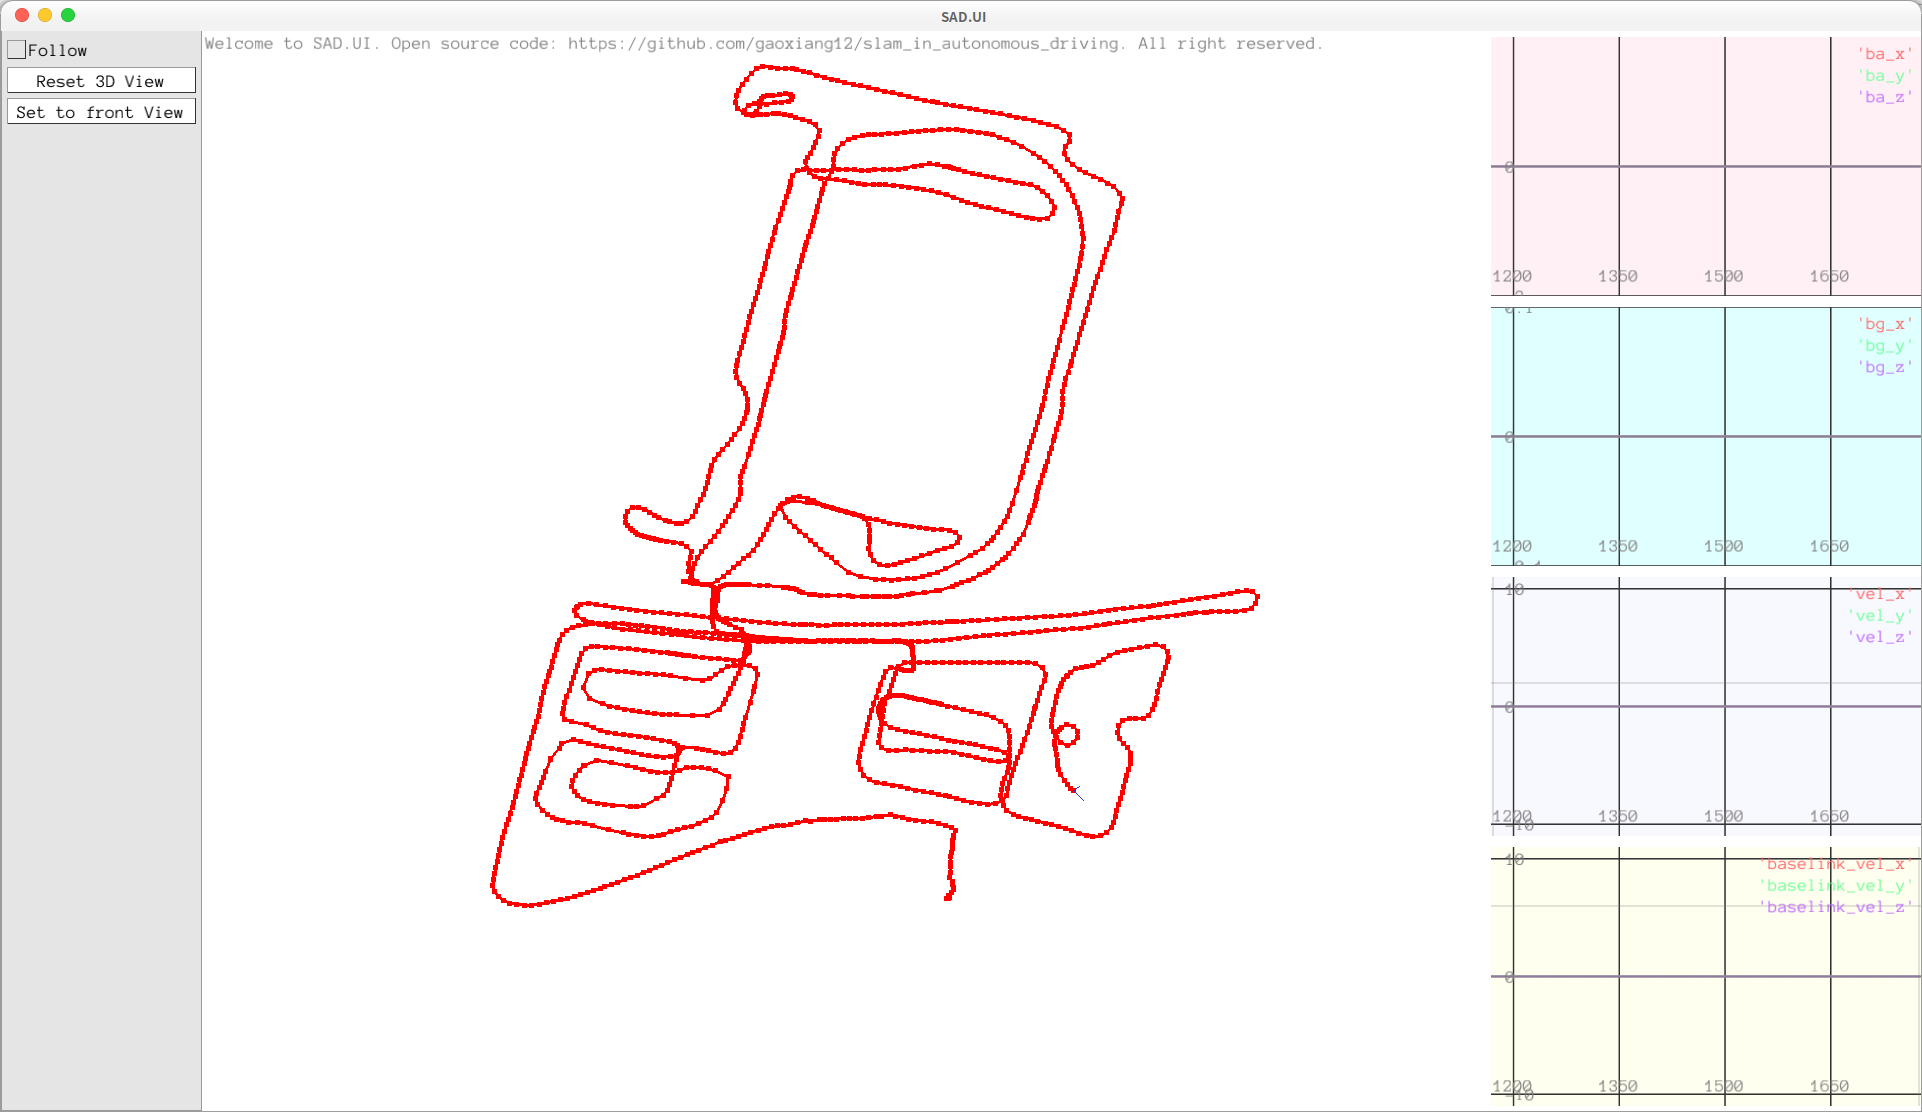
\includegraphics[width=1.0\textwidth]{ins/ch3-process-gnss.png}
%	\caption{GNSS的实时轨迹}
%	\label{fig:process-gnss}
%\end{figure}
%
%注意本节仅使用了RTK设备提供的位置与方向角信息。也有的RTK或组合导航设备内部集成了IMU,
%可以直接向外输出角速度、线速度等物理量。不过本书的目标在于介绍其原理,所以在此不直接使用RTK
%设备带来的这些信息了。
%
%\section{使用误差状态卡尔曼滤波器实现组合导航}
%RTK设备为我们提供了一个不太稳定的位姿观测源。我们可以将它直接视为定位滤波器的一种观测。
%本节我们来将RTK与IMU结合,使用拓展卡尔曼滤波器形成传统的组合导航算法,以供后续的算
%法作为对比。严格来说,我们向读者介绍的是\textbf{误差状态}的拓展卡尔曼滤波器(Error state Kalman 
%filter, ESKF)。ESKF的应用十分广泛,从GINS组合导航到视觉SLAM\cite{Kleinert2010,Li2013,Davison2003}、外参自标定\cite{Kelly2011,Mirzaei2008}等任务中都有应用。 为什么需要ESKF呢?ESKF与EKF之间又有何区别呢?我们会从动机层面开始介绍。这种由简至繁的过程也可以帮助
%读者更好地理清各种算法的发展过程。
%
%\subsection{ESKF的数学推导}
%前面我们已经介绍过IMU器件的观测模型了,现在我们需要把IMU视为运动模型,并把GNSS观测视
%为观测模型,推导整个滤波器。这件事情并不难。
%
%我们设状态变量为:
%\begin{equation}\label{key}
%\bm{x} = [\bm{p}, \bm{v}, \bm{R}, \bm{b}_g, \bm{b}_a, \bm{g}]^\top,
%\end{equation}
%所有变量都默认取下标$()_{WB}$,其中$\bm{p}$为平移,$\bm{v}$为速度,$\bm{R}$为旋转,$\bm{b}_g,
% \bm{b}_a$为零偏,$\bm{g}$为重力。按照我们前面介绍的运动学方程式\eqref{eq:motion-equation}并代入IMU测量值,状态变量在连续时间下的运
%动方程为:
%\begin{subequations}\label{eq:ekf-continous}
%\begin{align}
%	\dot{\bm{p}} &= \bm{v}, \\
%	\dot{\bm{v}} &= \bm{R} (\tilde{\bm{a}} - \bm{b}_{a} - \boldsymbol{\eta}_a) + \bm{g}, \\
%	\dot{\bm{R}} &= \bm{R} \left( \tilde{\boldsymbol{\omega}} - \bm{b}_{g} - \boldsymbol{\eta}_g 
%	\right)^\wedge, \\
%	\dot{\bm{b}}_{g} & = \boldsymbol{\eta}_{bg}, \\
%	\dot{\bm{b}}_{a} & = \boldsymbol{\eta}_{ba}, \\ 
%	\dot{\bm{g}} &= \bm{0}.
%\end{align}
%\end{subequations}
%
%为了在EKF的预测过程中对协方差进行预测,我们需要对该方程进行线性化。理论上,离散时间线性化的形式为:
%\begin{equation}\label{key}
%\bm{x}_{k+1} = \bm{f} (\bm{x}_k) + \bm{F} \mathrm{d} \bm{x} + \bm{w},
%\end{equation}
%其中$\bm{F} = \left. \frac{\partial \bm{f}}{\partial \bm{x}} \right|_{\bm{x}_{k}}$为系数矩阵。该矩阵由
%运动方程和各项状态变量的导数构成。然而,这里我们遇到了一个非常现实的问题:一方面,$\bm{F}$当中需
%要计算旋转矩阵$\bm{R}$相对于某个扰动的导数,而在不引入张量的情况下,是无法表达矩阵对向量导
%数的形式的。于是,传统算法往往会退一步,用欧拉角或者四元数的四个标量作为状态变量\cite{crassidis2006sigma},但这样
%就无法优雅地使用流形上的方法了。另一方面,如果我们考虑将惯性导航系统与卫星导航系统进行融合,那么$\bm{x}$中的平移变量就应该使用全局坐标系。这会使得$\bm{x}$中的数值变得很大,在有些场合超出浮点数的有效数字范围。这将导致一些常见的运算可能会失效,例如数值计算中的“大数吃小数”现象\cite{bonnans2006numerical}。
%
%于是,我们会说,能否避免直接使用$\bm{x}$和$\bm{P}$来表达状态的均值和协方差,来推导运动和观测方程?能否使用原先卡尔曼滤波器中的\textbf{更新量}来推导这两个方程?我们回忆卡尔曼滤波器中的观测部分:
%\begin{equation}\label{key}
%\bm{x}_k = \bm{x}_{k, \text{pred}} + \bm{K}_k \underbrace{(\bm{z}_k - \bm{H}_k \bm{x}_{k, \text{pred}})}_{\text{更新量}}.
%\end{equation}
%
%在流形意义下,右侧的更新量应是位于切空间中的矢量,中间的加法应为流形与切空间指数映射的广义加法。但我们也可以将更新量(或者称为误差状态)视为滤波器的状态变量,来推导运动和观测模型。这就引出了\textbf{误差状态卡尔曼滤波器}。更进一步,不光是平移和旋转,我们索性把所有的状态都用误差状态来表达,这就是典型ESKF的做法。
%
%ESKF是许多传统的、现代的系统里都广泛使用的状态估计方法,既可以作为组合导航的滤波器,也
%可以用来实现LIO、VIO等复杂系统\cite{Xu2021,xu2021fast, Bloesch2017}。相比于传统KF,ESKF的优点可以总
%结如下\cite{Madyastha2011}:
%\begin{enumerate}
%	\item 在旋转的处理上,ESKF的状态变量可以采用最小化的参数表达,也就是使用三维变量来表达
%	旋转的增量。该变量位于切空间中,而切空间是一个矢量空间。传统KF需要用到四元数(4维)或者更高维的变量来表达状态(旋转矩阵,9维),要不就得
%	采用带有奇异性的表达方式(欧拉角)。
%	\item ESKF总是在原点附近,离奇异点较远,数值方面更加稳定,并且也不会产生离工作点太远而导致线性化近似不够的问题。
%	\item ESKF的状态量为小量,其二阶变量相对来说可以忽略。同时大多数雅可比矩阵在小量情况下变得非常简单,甚至可以用单位阵代替。
%	\item 误差状态的运动学也相比原状态变量要来得更小(小量的运动学),因此我们可以把更新部分返回到原状态变量中。
%\end{enumerate}
%
%在ESKF中,我们通常把原状态变量称为\textbf{名义状态变量}(nominal state),然后把ESKF里的
%状态变量称为\textbf{误差状态变量}(error state)。名义状态变量和误差状态变量之和称为\textbf{真
%值}。我们把噪声的处理放到误差状态变量中,可以认为名义状态变量的方程是不含噪声的。这种做
%法在初次接触时会显得相对复杂,但将噪声分离之后,名义状态变量的方程反而变得简洁了。所谓的
%滤波器,也仅需要考虑误差状态如何运动,如何观测,最后如何进行滤波,和名义状态的关系不大。
%
%ESKF整体流程如下:当IMU测量数据到达时,我们把它积分后,放入名义状态变量中。由于这种做
%法没有考虑噪声,其结果自然会快速漂移,于是我们把误差部分作为误差变量。在运动过程中,名义状态随着IMU数据进行递推,误差状态则受到高斯噪声影响而变大。此时,ESKF的误差状态均值和协方差会描述误差状态扩大的具体数值(视为高斯分布)\footnote{但是后文我们将看到,由于各项噪声均为零均值的白噪声,误差状态的均值在运动方程中保持为零,只是协方差会增大。}。此外,ESKF的更新过程需要依赖IMU以外的传感器观测。更新过程中,我们利用传感器数据,更新误差状态的\textbf{后验}均值与协方差。随后我们可以把这部分误差\textbf{合入}名义状态变量中,并把ESKF置零,这样就完成了一次预测——更新的循环。
%
%下面来推导ESKF的两个过程。我们设ESKF的真值状态为:$\bm{x}_t = [\bm{p}_t, \bm{v}_t, \bm{R}_t, \bm{b}_{at}, \bm{b}_{gt}, 
%\bm{g}_t]^\top$。下标$t$表示$\text{true}$,即真值状态。这个状态随时间改变,可以记$\bm{x}_t(t)$。在连续时间上,我们记IMU读
%数为$\tilde{\boldsymbol{\omega}}, \tilde{\bm{a}}$,那么根据之前的推导,我们可以写出状态变量导
%数相对于观测量之间的关系式:
%\begin{subequations}\label{eq:eskf-true-state}
%	\begin{align}
%		\dot{\bm{p}}_t &= \bm{v}_t, \\
%		\dot{\bm{v}}_t &= \bm{R}_t (\tilde{\bm{a}} - \bm{b}_{at} - \boldsymbol{\eta}_a) + \bm{g}_t, \\
%		\dot{\bm{R}}_t &= \bm{R}_t \  \left( \tilde{\boldsymbol{\omega}} - \bm{b}_{gt} - 
%		\boldsymbol{\eta}_g \right)^\wedge, \\
%		\dot{\bm{b}}_{gt} & = \boldsymbol{\eta}_{bg}, \\
%		\dot{\bm{b}}_{at} & = \boldsymbol{\eta}_{ba}, \\ 
%		\dot{\bm{g}}_t &= \bm{0}.
%	\end{align}
%\end{subequations}
%
%该式和前面所述的式\eqref{eq:ekf-continous}是一致的。注意这里把重力$\bm{g}$考虑进来的
%主要理由是方便确定IMU的初始姿态。如果我们不在状态方程里写出重力变量,那么必须事先确定初
%始时刻的IMU朝向$\bm{R}(0)$,才可以执行后续的计算。此时IMU的姿态是相对于初始的水平面来
%描述的。而如果把重力写出来,就可以设IMU的初始姿态为单位矩阵$\bm{R}=\bm{I}$,把重力方向
%作为IMU当前姿态相比于水平面的一个度量。二种方法都是可行的,不过将重力方向单独表达出来会
%使得初始姿态表达更加简单,同时还可以增加一些线性性\cite{Lupton2009}。
%
%如果我们把观测量和噪声量整理成一个向量,就可以把上式整理成矩阵形式。不过这样的矩阵形式将
%含有很多的零项,相比上式并不会有明显简化,所以我们就先使用这种散开的公式。下面我们来推导
%误差状态方程。首先定义误差状态变量为:
%\begin{subequations}\label{eq:eskf-true-to-error}
%	\begin{align}
%		\bm{p}_t &= \bm{p} + \delta \bm{p}, \\
%		\bm{v}_t &= \bm{v} + \delta \bm{v}, \\
%		\bm{R}_t &= \bm{R} \delta \bm{R} \quad  \text{或} \ \bm{q}_t = \bm{q} \delta \bm{q}, \\
%		\bm{b}_{gt} &= \bm{b}_g + \delta \bm{b}_g, \\
%		\bm{b}_{at} &= \bm{b}_a + \delta \bm{b}_a, \\
%		\bm{g}_t &= \bm{g} + \delta \bm{g}.
%	\end{align}
%\end{subequations}
%
%不带下标的就是式(\ref{eq:eskf-true-state})中的\textbf{名义状态变量}。名义状态变量的运动学方程
%式与真值相同,只是\textbf{不必考虑噪声}(因为噪声在误差状态方程中考虑了)。其中旋转部分的$\delta
% \bm{R}$可以用它的李代数$\mathrm{Exp}(\delta \boldsymbol{\theta})$来表示,此时(c)式也需要改成
%用指数形式来表达。
%
%在误差状态的(a,d,e,f)式中,在等式两侧分别对时间求导,很容易能得到对应的时间导数表达式:
%\begin{subequations}
%	\begin{align}
%		\delta \dot{\bm{p}} &= \delta \bm{v}, \\
%		\delta \dot{\bm{b}_g} &= \boldsymbol{\eta}_{bg}, \\
%		\delta \dot{\bm{b}_a} &= \boldsymbol{\eta}_{ba}, \\
%		\delta \dot{\bm{g}} &= \bm{0}.
%	\end{align}
%\end{subequations}
%而(b),(c)两式由于和$\delta \bm{R}$有关系,形式稍微复杂一些,下面给出单独的推导。
%
%
%\subsubsection{误差状态的旋转项}
%对式(\ref{eq:eskf-true-to-error})(c)两侧求时间导数,可得:
%\begin{equation}\label{eq:eskf-3.19}
%	\begin{aligned}
%		\dot{\bm{R}}_t &= \dot{\bm{R}} \mathrm{Exp} (\delta \boldsymbol{\theta}) + \bm{R} 
%		\dot{\mathrm{Exp}(\delta \boldsymbol{\theta})},  \\
%		&\buildrel{\ref{eq:eskf-true-state}(c)}\over=  \bm{R}_t \left( \tilde{\boldsymbol{\omega}} - 
%		\bm{b}_{gt} - \boldsymbol{\eta}_g \right) ^\wedge.
%	\end{aligned}
%\end{equation}
%
%注意到该式右边的$\dot{\mathrm{Exp}(\delta \boldsymbol{\theta})}$满足:
%\begin{equation}
%	\dot{\mathrm{Exp}(\delta \boldsymbol{\theta})} = \mathrm{Exp}(\delta \boldsymbol{\theta}) \delta 
%	\dot{\boldsymbol{\theta}}^\wedge.
%\end{equation} 
%因此\eqref{eq:eskf-3.19}的第一个式子可写成:
%\begin{equation}\label{key}
%	\dot{\bm{R}} \mathrm{Exp} (\delta \boldsymbol{\theta}) + \bm{R} \dot{\mathrm{Exp}(\delta 
%	\boldsymbol{\theta})} = \bm{R} (\tilde{\boldsymbol{\omega}}-\bm{b}_g)^\wedge 
%	\mathrm{Exp}(\delta \boldsymbol{\theta}) + \bm{R} \mathrm{Exp}(\delta \boldsymbol{\theta} ) 
%	\delta \dot{\boldsymbol{\theta}}^\wedge.
%\end{equation}
%
%而第二个式子可以写成:
%\begin{equation}\label{key}
%	\begin{aligned}
%		\bm{R}_t \left( \tilde{\boldsymbol{\omega}} - \bm{b}_{gt} - \boldsymbol{\eta}_g \right)^\wedge 
%		&= \bm{R}  \mathrm{Exp} (\delta \boldsymbol{\theta}) \left( \tilde{\boldsymbol{\omega}} - 
%		\bm{b}_{gt} - \boldsymbol{\eta}_g \right)^\wedge.
%	\end{aligned}
%\end{equation}
%
%比较这两个式子,将$\delta \dot{\boldsymbol{\theta}}^\wedge$移到一侧,约掉两侧左边的$\bm{R}$,整理类
%似项,不难得到:
%\begin{equation}
%	\begin{aligned}
%		\mathrm{Exp} (\delta \boldsymbol{\theta}) \delta \dot{\boldsymbol{\theta}}^\wedge &= 
%		\mathrm{Exp} (\delta \boldsymbol{\theta}) \left( \tilde{\boldsymbol{\omega}} - \bm{b}_{gt} - 
%		\boldsymbol{\eta}_g \right)^\wedge - (\tilde{\boldsymbol{\omega}}-\bm{b}_g)^\wedge 
%		\mathrm{Exp}(\delta \boldsymbol{\theta}).
%	\end{aligned}
%\end{equation}
%
%注意到$\mathrm{Exp}(\delta 
%\boldsymbol{\theta})$本身是一个$\mathrm{SO}(3)$矩阵,我们利用$\mathrm{SO}(3)$上的伴随性质:
%\begin{equation}\label{key}
%	\boldsymbol{\phi}^\wedge \bm{R} = \bm{R} (\bm{R}^\top \boldsymbol{\phi})^\wedge
%\end{equation}
%来交换上面的$\mathrm{Exp}(\delta \boldsymbol{\theta})$:
%\begin{equation}\label{key}
%	\begin{aligned}
%		\mathrm{Exp} (\delta \boldsymbol{\theta}) \delta \dot{\boldsymbol{\theta}}^\wedge &= 
%		\mathrm{Exp} (\delta \boldsymbol{\theta}) \left( \tilde{\boldsymbol{\omega}} - \bm{b}_{gt} - 
%		\boldsymbol{\eta}_g \right)^\wedge - \mathrm{Exp} (\delta \boldsymbol{\theta})  \left( 
%		\mathrm{Exp} (-\delta \boldsymbol{\theta})  (\tilde{\boldsymbol{\omega}}-\bm{b}_g) 
%		\right)^\wedge \\
%		&=  \mathrm{Exp} (\delta \boldsymbol{\theta}) \left[ (\tilde{\boldsymbol{\omega}} - \bm{b}_{gt} - 
%		\boldsymbol{\eta}_g)^\wedge - (\mathrm{Exp} (-\delta \boldsymbol{\theta})  
%		(\tilde{\boldsymbol{\omega}}-\bm{b}_g) )^\wedge \right] \\
%		&\approx \mathrm{Exp} (\delta \boldsymbol{\theta}) \left[ (\tilde{\boldsymbol{\omega}} - 
%		\bm{b}_{gt} - \boldsymbol{\eta}_g)^\wedge - \left((\bm{I} - \delta 
%		\boldsymbol{\theta}^\wedge)(\tilde{\boldsymbol{\omega}}-\bm{b}_g )\right)^\wedge \right] \\
%		&=  \mathrm{Exp} (\delta \boldsymbol{\theta}) \left[ \bm{b}_g - \bm{b}_{gt} -\boldsymbol{\eta}_g 
%		+ \delta \boldsymbol{\theta}^\wedge \tilde{\boldsymbol{\omega}} - \delta 
%		\boldsymbol{\theta}^\wedge \bm{b}_{g} \right]^\wedge \\
%		&= \mathrm{Exp} (\delta \boldsymbol{\theta}) \left[ 
%		(-\tilde{\boldsymbol{\omega}}+\bm{b}_g)^\wedge \delta \boldsymbol{\theta} - \delta \bm{b}_g - 
%		\boldsymbol{\eta}_g \right]^\wedge.
%	\end{aligned}
%\end{equation}
%
%
%约掉等式左侧的系数,可得:
%\begin{equation}\label{key}
%	\delta \dot{\boldsymbol{\theta}} \approx -(\tilde{\boldsymbol{\omega}} - \bm{b}_g)^\wedge \delta 
%	\boldsymbol{\theta} - \delta \bm{b}_g - \boldsymbol{\eta}_g. 
%\end{equation}
%
%该式的$\approx$来自于$\mathrm{Exp}(-\delta \boldsymbol{\theta})$的展开,如果忽略$\delta \boldsymbol{\theta}$的二阶小量,上式也可以写成等号。
%
%\subsubsection{误差状态的速度项}
%接下来考虑式(\ref{eq:eskf-true-to-error})(b)的误差形式。同样地,对两侧求时间导数,就可以得到$\delta
% \dot{\bm{v}}$的表达式。等式左侧为:
%\begin{equation}
%	\begin{aligned}
%		\dot{\bm{v}}_t &= \bm{R}_t(\tilde{\bm{a}} - \bm{b}_{at} - \boldsymbol{\eta}_a) + \bm{g}_t \\
%		&= \bm{R} \mathrm{Exp}(\delta \boldsymbol{\theta}) (\tilde{\bm{a}} - \bm{b}_a - \delta \bm{b}_a 
%		- \boldsymbol{\eta}_a ) + \bm{g} + \delta \bm{g} \\
%		&\approx \bm{R} (\bm{I} + \delta \boldsymbol{\theta}^\wedge ) (\tilde{\bm{a}} - \bm{b}_a - \delta 
%		\bm{b}_a - \boldsymbol{\eta}_a) + \bm{g} + \delta \bm{g} \\
%		&\approx \bm{R} \tilde{\bm{a}} - \bm{R} \bm{b}_a - \bm{R} \delta \bm{b}_a - \bm{R} 
%		\boldsymbol{\eta}_a + \bm{R} \delta \boldsymbol{\theta}^\wedge \tilde{\bm{a}} - \bm{R} \delta 
%		\boldsymbol{\theta}^\wedge \bm{b}_a + \bm{g} + \delta \bm{g} \\
%		&= \bm{R} \tilde{\bm{a}} - \bm{R} \bm{b}_a - \bm{R} \delta \bm{b}_a - \bm{R} 
%		\boldsymbol{\eta}_a - \bm{R} \tilde{\bm{a}}^\wedge \delta \boldsymbol{\theta}  + \bm{R} 
%		\bm{b}_a^\wedge  \delta\boldsymbol{\theta}  + \bm{g} + \delta \bm{g}.
%	\end{aligned}
%\end{equation}
%从第三行推向第四行时,也需要忽略$\delta \boldsymbol{\theta}^\wedge$与$\delta \bm{b}_a, 
%\boldsymbol{\eta}_a$相乘的二阶小量。从第四行推第五行则用到了叉乘符号交换顺序之后需加负号
%的性质。另一方面,等式右侧为:
%
%\begin{equation}\label{key}
%	\dot{\bm{v}} + \delta \dot{\bm{v}} = \bm{R}(\tilde{\bm{a}} - \bm{b}_a) + \bm{g} + \delta \dot{\bm{v}}.
%\end{equation}
%
%因为上面两式相等,可以得到:
%\begin{equation}\label{key}
%	\delta \dot{\bm{v}} = - \bm{R}(\tilde{\bm{a}} - \bm{b}_a)^\wedge \delta \boldsymbol{\theta} - 
%	\bm{R} \delta \bm{b}_a  - \bm{R} \boldsymbol{\eta}_a + \delta \bm{g}.
%\end{equation}
%
%这样我们就得到了$\delta \bm{v}$的运动学模型。需要补充一句,由于上式中$\boldsymbol{\eta}_a$
%是一个零均值白噪声,它乘上任意旋转矩阵之后仍然是一个零均值白噪声,而且由于$\bm{R}^\top
% \bm{R} = \bm{I}$,容易证明其协方差矩阵也不变(留作习题)。所以,也可以把上式简化为:
%\begin{equation}\label{key}
%	\delta \dot{\bm{v}} = - \bm{R}(\tilde{\bm{a}} - \bm{b}_a)^\wedge \delta \boldsymbol{\theta} - 
%	\bm{R} \delta \bm{b}_a  - \boldsymbol{\eta}_a + \delta \bm{g}.
%\end{equation}
%
%至此,我们可以把误差变量的运动学方程整理如下:
%\begin{subequations}\label{eq:eskf-error-state-continuous-time}
%	\begin{align}
%		\delta \dot{\bm{p}} &= \delta \bm{v}, \\
%		\delta \dot{\bm{v}} &= - \bm{R}(\tilde{\bm{a}} - \bm{b}_a)^\wedge \delta \boldsymbol{\theta} - 
%		\bm{R} \delta \bm{b}_a  - \boldsymbol{\eta}_a + \delta \bm{g}, \\
%		\delta \dot{\boldsymbol{\theta}} &= -(\tilde{\boldsymbol{\omega}} - \bm{b}_g)^\wedge \delta 
%		\boldsymbol{\theta} - \delta \bm{b}_g - \boldsymbol{\eta}_g, \\
%		\delta \dot{\bm{b}_g} &= \boldsymbol{\eta}_{bg}, \\
%		\delta \dot{\bm{b}_a} &= \boldsymbol{\eta}_{ba}, \\
%		\delta \dot{\bm{g}} &= \bm{0} .
%	\end{align}
%\end{subequations}
%
%\subsection{离散时间的ESKF运动学方程}
%从连续时间状态方程推出离散时间的状态方程并不困难,不妨直接来列写它们。\textbf{名义状态变量}的离散
%时间运动学方程可以写为:
%\begin{subequations}\label{key}
%	\begin{align}
%		\bm{p}(t+\Delta t) &= \bm{p}(t) + \bm{v} \Delta t + \frac{1}{2} 
%		\left(\bm{R}(\tilde{\bm{a}}-\bm{b}_a) \right) \Delta t^2 + \frac{1}{2} \bm{g} \Delta t^2, \\
%		\bm{v}(t+\Delta t) &= \bm{v}(t) + \bm{R} (\tilde{\bm{a}} - \bm{b}_a) \Delta t + \bm{g} \Delta t,	\\
%		\bm{R}(t+\Delta t) &= \bm{R}(t) \mathrm{Exp} \left( (\tilde{\boldsymbol{\omega}}-\bm{b}_g) 
%		\Delta t \right),\\
%		\bm{b}_g(t+\Delta t) &= \bm{b}_g(t), \\
%		\bm{b}_a(t+\Delta t) &= \bm{b}_a(t), \\
%		\bm{g}(t+\Delta t) &= \bm{g}(t) .
%	\end{align}
%\end{subequations}
%该式只需在式\eqref{eq:3.14}基础上添加零偏项与重力项即可。注意第三行实际就是角速度的积分公式。\textbf{误差状态}的离散形式与\textbf{名义状态}十分相似,同样需要注意角速度部分:
%
%\begin{subequations}\label{eq:eskf-motion-equation}
%	\begin{align}
%		\delta \bm{p}(t+\Delta t) &= \delta \bm{p} + \delta \bm{v} \Delta t, \\
%		\delta \bm{v}(t+\Delta t) &= \delta \bm{v} + \left( - \bm{R}(\tilde{\bm{a}} - \bm{b}_a)^\wedge 
%		\delta \boldsymbol{\theta} - \bm{R} \delta \bm{b}_a  + \delta \bm{g} \right) \Delta t -
%		\boldsymbol{\eta}_{v}, \\
%		\delta \boldsymbol{\theta} (t+\Delta t) &= \mathrm{Exp}\left( -(\tilde{\boldsymbol{\omega}} - 
%		\bm{b}_g) \Delta t \right) \delta \boldsymbol{\theta} - \delta \bm{b}_g \Delta t - 
%		\boldsymbol{\eta}_{\theta}, \\
%		\delta \bm{b}_g (t+\Delta t) &= \delta \bm{b}_g + \boldsymbol{\eta}_{bg}, \\
%		\delta \bm{b}_a (t+\Delta t)&= \delta \bm{b}_a + \boldsymbol{\eta}_{ba}, \\
%		\delta \bm{g} (t+\Delta t) &= \delta \bm{g}.
%	\end{align}
%\end{subequations}
%
%注意:
%\begin{enumerate}
%	\item 右侧部分我们省略了括号里的$(t)$以简化公式;
%	\item 关于旋转部分的积分,我们可以将式\eqref{eq:eskf-error-state-continuous-time}(c)看成
%	关于$\delta \boldsymbol{\theta}$的微分方程然后求解。求解过程类似于对角速度进行积分。
%	\item 噪声项并不参与递推,需要把它们单独归入噪声部分中。连续时间的噪声项可以视为随机过
%	程的能量谱密度,而离散时间下的噪声变量就是我们日常看到的随机变量了。这些噪声随机变量的
%	标准差可以列写如下:
%	\begin{equation}\label{key}
%		\sigma(\boldsymbol{\eta}_v) = \Delta t \sigma_a(k), \quad \sigma(\boldsymbol{\eta}_{\theta}) = 
%		\Delta t \sigma_{g}(k), \quad \sigma(\boldsymbol{\eta}_{bg}) = \sqrt{\Delta t} \sigma_{bg}, \quad  
%		\sigma(\boldsymbol{\eta}_{ba}) = \sqrt{\Delta t} \sigma_{ba},
%	\end{equation}
%	其中前两式的$\Delta t$是由积分关系导致的,后面两式则和\eqref{eq:imu-noise-relationship}相同。
%\end{enumerate}
%
%至此,我们给出了如何在ESKF中进行IMU递推的过程,对应于卡尔曼滤波器中的状态方程。为了让
%滤波器收敛,我们需要外部的观测来对卡尔曼滤波器进行修正,也就是所谓的组合导航。当然,
%组合导航的方法有很多,从传统的EKF,到本节介绍的ESKF,以及后续章节将要介绍预积分和图优
%化技术,都可以应用于组合导航中\cite{Wen2021}。本节,我们以融合GNSS观测为例,向读者介绍如何在ESKF中
%融合这些观测数据,形成一个收敛的卡尔曼滤波器。在本书最后的应用章节中,也将向读者介绍融合激光点云
%或者激光定位数据的滤波器方案。
%
%\subsection{ESKF的运动过程}
%根据上述讨论,我们可以写出ESKF的运动过程。误差状态变量$\delta \bm{x}$的离散时间运动方程
%已经在式\eqref{eq:eskf-motion-equation}给出,我们可以整体地记为:
%\begin{equation}\label{key}
%	\delta \bm{x}_{k+1} = \bm{f} (\delta \bm{x}_{k}) + \bm{w}, \bm{w} \sim \mathcal{N}(0, \bm{Q}),
%\end{equation}
%其中$\bm{w}$为噪声。按照前面的定义,$\bm{Q}$应该为:
%\begin{equation}\label{key}
%	\bm{Q} = \mathrm{diag}(\bm{0}_3, \mathrm{Cov}(\boldsymbol{\eta}_v), 
%	\mathrm{Cov}(\boldsymbol{\eta}_{\theta}), \mathrm{Cov}(\boldsymbol{\eta}_{g}), 
%	\mathrm{Cov}(\boldsymbol{\eta}_{a}), \bm{0}_3),
%\end{equation}
%两侧的零是由于第一个和最后一个方程本身没有噪声导致的。
%
%为了保持与EKF的符号统一,我们计算运动方程的线性化形式:
%\begin{equation}\label{key}
%	\delta \bm{x}(t+\Delta t) = \underbrace{\bm{f}(\delta \bm{x}(t))}_{=\bm{0}} + \bm{F} \delta \bm{x} + \bm{w},
%\end{equation}
%其中$\bm{F}$为线性化后的雅可比矩阵。由于式\eqref{eq:eskf-motion-equation}已经是线性化的了,
%现在我们只需把它们的线性系数拿出来,只是要注意变量定义的顺序:
%\begin{equation}\label{eq:eskf-F}
%	\bm{F} = \begin{bmatrix}
%		\bm{I} & \bm{I} \Delta t & \bm{0} & \bm{0} & \bm{0} & \bm{0} \\
%		\bm{0} & \bm{I} & - \bm{R}(\tilde{\bm{a}} - \bm{b}_a)^\wedge \Delta t & \bm{0} & -\bm{R} \Delta t & \bm{I} \Delta t \\
%		\bm{0} & \bm{0} & \mathrm{Exp}\left( -(\tilde{\boldsymbol{\omega}} - \bm{b}_g) \Delta t \right) 
%		&  -\bm{I} \Delta t & \bm{0} & \bm{0} \\
%		\bm{0} & \bm{0} & \bm{0} & \bm{I} & \bm{0} & \bm{0} \\
%		\bm{0} & \bm{0} & \bm{0} & \bm{0} & \bm{I} & \bm{0} \\
%		\bm{0} & \bm{0} & \bm{0} & \bm{0} & \bm{0} & \bm{I} 
%	\end{bmatrix}.
%\end{equation}
%
%在此基础上,我们执行ESKF的预测过程。预测过程包括对名义状态的预测(IMU积分)以及对误差
%状态的预测:
%\begin{subequations}\label{eq:motion-eskf}
%	\begin{align}
%		\delta \bm{x}_{\mathrm{pred}} &= \bm{F} \delta \bm{x}, \\
%		\bm{P}_{\mathrm{pred}} &= \bm{F} \bm{P} \bm{F}^\top + \bm{Q}.
%	\end{align}
%\end{subequations}
%
%不过由于ESKF的误差状态在每次更新以后会被重置为$\delta \bm{x} = \bm{0}$,因此运动方程的均值部分,即\eqref{eq:motion-eskf}(a) 没有太大意义,而协方差部分则描述了整个误差估计的分布情况。在直观意义上,运动方程的噪声协方差中增加了$\bm{Q}$项,可以看作是\textbf{增大}的过程。
%
%\subsection{ESKF的更新过程}
%\label{subsec:3.4.4}
%前面介绍的是ESKF的运动过程,现在我们来考虑更新过程。假设一个抽象的传感器能够对状态变量
%产生观测,其观测方程为抽象的$\bm{h}$,那么可以写为:
%\begin{equation}\label{key}
%	\bm{z} = \bm{h} (\bm{x}) + \bm{v}, \bm{v} \sim \mathcal{N}(0, \bm{V}),
%\end{equation}
%其中$\bm{z}$为观测数据, $\bm{v}$为观测噪声,$\bm{V}$为该噪声的协方差矩阵\footnote{由于状
%态变量里已经有$\bm{R}$了,这里我们换个符号。}。
%
%在传统EKF中,我们可以直观对观测方程线性化,求出观测方程相对于状态变量的雅可比矩阵,进而
%更新卡尔曼滤波器。而在ESKF中,我们当前拥有名义状态$\bm{x}$的估计以及误差状态$\delta 
%\bm{x}$的估计,且希望更新的是误差状态,因此要计算观测方程相对于误差状态的雅可比矩阵:
%\begin{equation}\label{key}
%	\bm{H} = \left. \frac{\partial \bm{h}}{\partial \delta \bm{x}} \right|_{\bm{x}_{\text{pred}}}, 
%\end{equation}
%然后再计算卡尔曼增益,进而计算误差状态的更新过程:
%\begin{subequations}\label{eq:eskf-obs-correction}
%	\begin{align}
%		\bm{K} &= \bm{P}_{\mathrm{pred}} \bm{H}^\top(\bm{H} \bm{P}_{\mathrm{pred}} 
%		\bm{H}^\top + \bm{V})^{-1}, \\
%		\delta \bm{x} &= \bm{K} (\bm{z} - \bm{h}(\bm{x}_{\mathrm{pred}})), \\
%		\bm{x} &= \bm{x}_{\text{pred}} + \delta \boldsymbol{\bm{x}}, \\
%		\bm{P} &= (\bm{I} - \bm{K} \bm{H}) \bm{P}_{\mathrm{pred}}.
%	\end{align}
%\end{subequations}
%其中$\bm{K}$为卡尔曼增益,$\bm{P}_{\mathrm{pred}}$为预测的协方差矩阵,最后的$\bm{P}$为修
%正后的协方差矩阵。
%
%大部分的观测数据是对名义状态的观测\footnote{但也有些情况下,我们可以直接推导对误差状态的观测,那么就能省略本节后续的推导。后续的GNSS观测和激光观测都会使用直接观测误差状态的方式来推导。}。此时$\bm{H}$可以通过链式法则来生成:
%\begin{equation}\label{eq:def-of-H}
%	\bm{H} = \frac{\partial \bm{h}}{\partial \bm{x}} \frac{\partial \bm{x}}{\partial \delta \bm{x}},
%\end{equation}
%其中第一项只需对观测方程进行线性化,第二项,根据我们之前对状态变量的定义,可以得到:
%\begin{equation}\label{key}
%	\frac{\partial \bm{x}}{\partial \delta \bm{x}} = \mathrm{diag}(\bm{I}_3, \bm{I}_3, \frac{\partial 
%	\mathrm{Log} (\bm{R}(\mathrm{Exp}(\delta \boldsymbol{\theta})))}{\partial \delta 
%	\boldsymbol{\theta}}, \bm{I}_3, \bm{I}_3, \bm{I}_3).
%\end{equation}
%其他几项都是平凡的,只有旋转部分,因为$\delta \boldsymbol{\theta}$定义为$\bm{R}$的右乘,我
%们用右乘的BCH即可:
%\begin{equation}\label{key}
%	\frac{\partial \mathrm{Log} (\bm{R}(\mathrm{Exp}(\delta \boldsymbol{\theta})))}{\partial \delta 
%	\boldsymbol{\theta}} = \bm{J}_r^{-1} (\bm{R}).
%\end{equation}
%最后,我们可以给每个变量加下标$k$,表示在$k$时刻进行状态估计,但本节没必要这样做,因为上述公式已经清楚地表明了它们的意义。另外,上述公式也都可以按照四元数的表达方式来推导,大致形式相似,细节方面要更加复杂一些,读者可以参考\cite{Sola2017}。本书正文部分只给出以$\mathrm{SO}(3)$及其李代数方式的推导。
%
%\subsection{ESKF的误差状态后续处理}
%在经过预测和更新过程之后,我们修正了误差状态的估计。接下来,只需把误差状态归入名义状态,
%然后重置ESKF即可。归入部分可以简单地写为:
%\begin{subequations}\label{key}
%	\begin{align}
%		\bm{p}_{k+1} &= \bm{p}_k + \delta \bm{p}_k, \\
%		\bm{v}_{k+1} &= \bm{v}_k + \delta \bm{v}_k, \\
%		\bm{R}_{k+1} &= \bm{R}_k \mathrm{Exp}(\delta \boldsymbol{\theta}_k), \\
%		\bm{b}_{g, k+1} &= \bm{b}_{g,k} + \delta \bm{b}_{g,k}, \\
%		\bm{b}_{a, k+1} &= \bm{b}_{a,k} + \delta \bm{b}_{a,k}, \\
%		\bm{g}_{k+1} &= \bm{g}_{k} + \delta \bm{g}_{k}.
%	\end{align}
%\end{subequations}
%有些文献里也会将上述计算定义为广义的状态变量加法:
%\begin{equation}\label{key}
%	\bm{x}_{k+1} = \bm{x}_k \oplus \delta \bm{x}_{k},
%\end{equation}
%这种写法可以简化整体的表达式,但会牺牲一定的可读性。如果公式里出现太多的广义加减法(特别是定义不同的广义加减$\oplus$、$\boxplus$、$\ominus$、$\boxminus$等),会让读者一眼望去,难以快速辨认它们的具体含义,所以本书还是倾向于将各状态分别写开,直接用加法而非广义加法符号。
%
%ESKF的重置分为均值部分和协方差部分。均值部分可以简单地实现为:
%\begin{equation}\label{key}
%	\delta \bm{x} = \bm{0}.
%\end{equation}
%由于均值被重置了,之前我们描述的是关于$\bm{x}_k$切空间中的协方差,而现在描述的是$\bm{x}_{k+1}$中的协方差。重置会带来一些微小的差异,主要影响旋转部分。事实上,在重置前,卡尔曼滤波器刻画了$\bm{x}_{\mathrm{pred}}$切空间处的一个高斯分布$\mathcal{N}(\delta \bm{x}, \bm{P})$,而重置之后,应该刻画$\bm{x}_{\mathrm{pred}} + \delta \bm{x}$处的一个$\mathcal{N}(0, \bm{P}_{\mathrm{reset}})$。这对本身即为矢量的状态是一样的,但对于旋转变量来说,它们的切空间零点发生了改变,所以在数学习惯上,需要对此进行区分。
%
%我们设重置前的名义旋转估计为$\bm{R}_k$,误差状态为$\delta \boldsymbol{\theta}$,卡尔曼滤波器的增量计算结果为$\delta \boldsymbol{\theta}_k$\footnote{注意此处$\delta \boldsymbol{\theta}_k$是已知的,而$\delta \boldsymbol{\theta}$是一个随机变量。};重置之后的名义旋转部分为$\bm{R}_k \mathrm{Exp}(\delta \boldsymbol{\theta}_k)=\bm{R}^+$,误差状态为$\delta \boldsymbol{\theta}^+$。由于误差状态被重置了,显然此时$\delta \boldsymbol{\theta}^+ = \bm{0}$。但我们关心的并不是它们直接的取值,而是$\delta \boldsymbol{\theta}^+$与$\delta \boldsymbol{\theta}$的线性化关系。把实际的重置过程写出来:
%\begin{equation}\label{key}
%	\bm{R}^+ \mathrm{Exp}(\delta \boldsymbol{\theta}^+) = \bm{R}_k \mathrm{Exp}(\delta \boldsymbol{\theta}_k) \mathrm{Exp}(\delta \boldsymbol{\theta}^+) = \bm{R}_k \mathrm{Exp}(\delta \boldsymbol{\theta}).
%\end{equation}
%
%不难得到:
%\begin{equation}\label{key}
%	\mathrm{Exp}(\delta \boldsymbol{\theta}^+) = \mathrm{Exp}(-\delta \boldsymbol{\theta}_k) \mathrm{Exp}(\delta \boldsymbol{\theta}),
%\end{equation}
%
%这里$\delta \boldsymbol{\theta}$为小量,利用线性化后的BCH公式,可以得到:
%\begin{equation}\label{key}
%	\delta \boldsymbol{\theta}^+ = -\delta \boldsymbol{\theta}_k + \delta \boldsymbol{\theta} - \frac{1}{2} \delta \boldsymbol{\theta}_k^\wedge \delta \boldsymbol{\theta} + o((\delta \boldsymbol{\theta})^2) .
%\end{equation}
%
%于是:
%\begin{equation}\label{key}
%	\frac{\partial \delta \boldsymbol{\theta}^+}{\partial \delta \boldsymbol{\theta}} \approx \bm{I} - \frac{1}{2} \delta \boldsymbol{\theta}_k^\wedge .
%\end{equation}
%
%该式表明重置前后的误差状态相差一个旋转方面的小雅可比矩阵,我们记作$\bm{J}_{\boldsymbol{\theta}} = \bm{I} - \frac{1}{2} \delta \boldsymbol{\theta}_k^\wedge $。把这个小雅可比阵放到整个状态变量维度下,并保持其他部分为单位矩阵,可以得到一个完整的雅可比矩阵:
%\begin{equation}\label{key}
%	\bm{J}_k = \mathrm{diag}(\bm{I}_3, \bm{I}_3, \bm{J}_{\boldsymbol{\theta}}, \bm{I}_3, \bm{I}_3, \bm{I}_3),
%\end{equation}
%因此,在把误差状态的均值归零同时,它们的协方差矩阵也应该进行线性变换:
%\begin{equation}\label{eq:tangent-space-projection}
%	\bm{P}_{\mathrm{reset}} = \bm{J}_k \bm{P} \bm{J}_k^\top.
%\end{equation}
%
%不过,由于$\delta \boldsymbol{\theta}_k$并不大,这里的$\bm{J}_k$仍然十分接近于单位矩阵,所以大部分材料里并不处理这一项,而是直接把前面估计的$\bm{P}$阵作为下一时刻的起点。但本书仍然要介绍这一点,并且会在后面第~\ref{cpt:tightly-lio}~章中继续讨论这个问题。该问题实际意义是做了\textbf{切空间投影},即把一个切空间中的高斯分布投影到另一个切空间中。在ESKF中,两者没有明显差异,但后文的迭代卡尔曼滤波器(IESKF)还会牵扯到在观测过程中多次变换切空间。与此相比,ESKF只有重置过程中的单次变换,原理更加简单。
%
%\section{实现ESKF的组合导航}
%下面我们通过代码来实现一个融合IMU与GNSS观测的ESKF。本节的代码仍然将结果输出到文本文
%件中,然后再调用可视化进行处理。在ESKF的实现过程中,我们还将遇到一些实现细节,我们会在本
%节讨论。
%
%\subsection{ESKF滤波器的实现}
%首先我们来定义ESKF的类。它的成员变量应该包含名义状态、误差状态、协方差,以及各类传感器噪声。
%
%\begin{lstlisting}[language=c++,caption=src/ch3/eskf.hpp]
%template <typename S = double>
%class ESKF {
%    /// 类型定义
%	using SO3 = Sophus::SO3<S>;                     // 旋转变量类型
%	using VecT = Eigen::Matrix<S, 3, 1>;            // 向量类型
%	using Vec18T = Eigen::Matrix<S, 18, 1>;         // 18维向量类型
%	using Mat3T = Eigen::Matrix<S, 3, 3>;           // 3x3矩阵类型
%	using MotionNoiseT = Eigen::Matrix<S, 18, 18>;  // 运动噪声类型
%	using OdomNoiseT = Eigen::Matrix<S, 3, 3>;      // 里程计噪声类型
%	using GnssNoiseT = Eigen::Matrix<S, 6, 6>;      // GNSS噪声类型
%	using Mat18T = Eigen::Matrix<S, 18, 18>;        // 18维方差类型
%	using NavStateT = NavState<S>;                  // 整体名义状态变量类型
%
%	/// 省略其他构造函数和成员函数
%private:
%	/// 成员变量
%	double current_time_ = 0.0;  // 当前时间
%	
%	/// 名义状态
%	VecT p_ = VecT::Zero();
%	VecT v_ = VecT::Zero();
%	SO3 R_;
%	VecT bg_ = VecT::Zero();
%	VecT ba_ = VecT::Zero();
%	VecT g_{0, 0, -9.8};
%	
%	/// 误差状态
%	Vec18T dx_ = Vec18T::Zero();
%	
%	/// 协方差阵
%	Mat18T cov_ = Mat18T::Identity();
%	
%	/// 噪声阵
%	MotionNoiseT Q_ = MotionNoiseT::Zero();
%	OdomNoiseT odom_noise_ = OdomNoiseT::Zero();
%	GnssNoiseT gnss_noise_ = GnssNoiseT::Zero();
%	
%	/// 标志位
%	bool first_gnss_ = true;  // 是否为第一个gnss数据
%	
%	/// 配置项
%	Options options_;
%};
%
%using ESKFD = ESKF<double>;
%using ESKFF = ESKF<float>;
%\end{lstlisting}
%
%按照前文推导,名义状态包含位置、速度、旋转、零偏和重力,误差状态对应它们的向量形式。误差状态变量应该为$3 \times 6=18$维向量,对应的协方差矩阵亦为$18 \times 18$维方阵。我们允许用户使用单精度或双精度的ESKF,它们在性能上有少许差别。浮点精度可以通过模板参数指定,所以我们的ESKF类是一个模板类。有的ESKF实现还允许用户自己定义变量维度和变量顺序,那样模板化之后会让整个类变得更复杂,比如\cite{Hertzberg2013}。本书仅定义float和double的ESKF类。ESKF内部用到的类型则通过using来指定。
%
%\subsection{实现预测过程}
%下面我们实现Predict函数,用于根据当前状态来对IMU数据进行递推。预测过程中,我们需要计算名义状态变量的更新过程以及
%协方差矩阵的递推过程,实现如下:
%\begin{lstlisting}[language=c++,caption=src/ch3/eskf.hpp]
%template <typename S>
%bool ESKF<S>::Predict(const IMU& imu) {
%	assert(imu.timestamp_ >= current_time_);
%	
%	double dt = imu.timestamp_ - current_time_;
%	if (dt > (5 * options_.imu_dt_) || dt < 0) {
%		// 时间间隔不对,可能是第一个IMU数据,没有历史信息
%		LOG(INFO) << "skip this imu because dt_ = " << dt;
%		current_time_ = imu.timestamp_;
%		return false;
%	}
%	
%	// nominal state 递推
%	VecT new_p = p_ + v_ * dt + 0.5 * (R_ * (imu.acce_ - ba_)) * dt * dt + 0.5 * g_ * dt * dt;
%	VecT new_v = v_ + R_ * (imu.acce_ - ba_) * dt + g_ * dt;
%	SO3 new_R = R_ * SO3::exp((imu.gyro_ - bg_) * dt);
%	
%	R_ = new_R;
%	v_ = new_v;
%	p_ = new_p;
%	// 其余状态维度不变
%	
%	// error state 递推
%	// 计算运动过程雅可比矩阵 F,见(3.47)
%	// F实际上是稀疏矩阵,也可以不用矩阵形式进行相乘而是写成散装形式,这里为了教学方便,使用矩阵形式
%	Mat18T F = Mat18T::Identity();                                                 // 主对角线
%	F.template block<3, 3>(0, 3) = Mat3T::Identity() * dt;                         // p 对 v
%	F.template block<3, 3>(3, 6) = -R_.matrix() * SO3::hat(imu.acce_ - ba_) * dt;  // v对theta
%	F.template block<3, 3>(3, 12) = -R_.matrix() * dt;                             // v 对 ba
%	F.template block<3, 3>(3, 15) = Mat3T::Identity() * dt;                        // v 对 g
%	F.template block<3, 3>(6, 6) = SO3::exp(-(imu.gyro_ - bg_) * dt).matrix();     // theta 对 theta
%	F.template block<3, 3>(6, 9) = -Mat3T::Identity() * dt;                        // theta 对 bg
%	
%	// mean and cov prediction
%	dx_ = F * dx_;  // 这行其实没必要算,dx_在重置之后应该为零,因此这步可以跳过,但F需要参与Cov部分计算,所以保留
%	cov_ = F * cov_.eval() * F.transpose() + Q_;
%	current_time_ = imu.timestamp_;
%	return true;
%}
%\end{lstlisting}
%
%这里我们写出了完整的$\bm{F}$矩阵,并使用矩阵方式进行协方差阵的更新。读者也可以不使用大的$\bm{F}$矩阵,而是单独的为每个状态变量计算分散的矩阵块。这对于一些稀疏矩阵可以节省一部分计算时间。我们看到,预测过程实质是使用IMU的读数,对名义状态进行递推。同时,在协方差矩阵层面合入运动过程的噪声,这样协方差矩阵就在直观意义下\textbf{变大}了。而误差状态在这一步的操作可以省略,因为观测过程会把误差状态置零,此时无论$\bm{F}$如何取值,$\bm{F} \delta \bm{x}$自然也就是零。运动过程是由IMU触发的,它可以被高频率调用,也可以输出高频率的预测位姿信息。
%
%\subsection{实现RTK观测过程}
%接下来我们考虑如何实现GNSS观测方程。这里我们认为RTK能够提供六自由度观测,即RTK既能观测位置,也能观测角度。注意单天线方案不能按照这种方式处理,应该使用三自由度的观测信息。
%
%观测方程的抽象形式是$\bm{y} = \bm{h}(\bm{x})$。我们曾在~\ref{subsec:3.4.4}~节中向大家介绍了通用的
%观测模型。而这里的GNSS观测数据,转换为车体UTM坐标以后,可以直接看作对当前$\bm{R}, \bm{p}$的观测。我们记某时刻的观测
%为$\bm{R}_{\mathrm{gnss}}, \bm{p}_{\mathrm{gnss}}$,来推导观测方程和卡尔曼增益部分。这里有以下几个要点:
%\begin{enumerate}
%	\item 在双天线方案中,车辆的角度由两个GNSS接收器决定。但可能存在部分时刻,一个GNSS有效而另一个GNSS无效,此时GNSS观测的位置是有效的,但航向角会失效。在本节处理中,我们只使用位置、角度同时有效的观测值。
%	\item GNSS对$\bm{R}$的观测可以直接写成对误差状态$\delta \boldsymbol{\theta}$的观测,从而省去前面的链式法则推导,简化整个线性化过程。
%	\item 此外,由于GNSS的UTM坐标一般数值较大,我们需要在实际处理时将去除RTK原点,以节省有效的数字位数。我们将
%	把第一个有效的GNSS观测记为原点,并让后续的GNSS位置观测都减去这个原点。这样,ESKF和后面可视化处理程序的坐标都将在零附近。有效数字过多可能导致绘图、可视化软件中的一些问题。
%\end{enumerate}
%
%现在我们来解释第2点。先看GNSS的旋转观测方程:
%\begin{equation}\label{eq:obs-gnss}
%\bm{R}_{\mathrm{gnss}} = \bm{R} \mathrm{Exp}(\delta \boldsymbol{\theta}),
%\end{equation}
%其中$\bm{R}$为该时刻的名义状态,$\delta \boldsymbol{\theta}$为误差状态。由于在观测过程中,名义状态$\bm{R}$是确定的。我们不妨将$\bm{R}_{\mathrm{gnss}}$直接视为对$\delta \boldsymbol{\theta}$的观测。我们对该方程稍作变换,可以写为:
%\begin{equation}
%	\bm{z}_{\delta \boldsymbol{\theta}} = \bm{h}(\delta \boldsymbol{\theta}) = \mathrm{Log} 
%	\left(\bm{R}^\top \bm{R}_{\mathrm{gnss}} \right).
%\end{equation}
%
%此时$\bm{z}_{\delta \boldsymbol{\theta}}$是对$\delta \boldsymbol{\theta}$的直接观测,所以它关于$\delta \boldsymbol{\theta}$的雅可比为单位阵:
%\begin{equation}\label{key}
%\frac{\partial \bm{z}_{\delta \boldsymbol{\theta}}}{\partial \delta \boldsymbol{\theta}} = \bm{I}.
%\end{equation}
%这样就避免了再从名义状态到误差状态进行转换的过程,可以直接得到对误差状态的雅可比矩阵。注
%意当我们这样做时,原本ESKF中的\textbf{更新量}(innovation)$\bm{z}-\bm{h}(\bm{x})$也应该写成流形的形式:
%\begin{equation}\label{key}
%\bm{z} - \bm{h}(\bm{x}) = [\bm{p}_{\mathrm{gnss}} - \bm{p}, 
%\mathrm{Log}(\bm{R}^\top \bm{R}_{\mathrm{gnss}})]^\top.
%\end{equation}
%
%因为$\delta \boldsymbol{\theta}$在预测之后仍为零,所以此时$\bm{h} (\bm{x})$的旋转部分视为零,平移部分则按照之前的定义来处理。这个更新量是6维的。我们用它来更新系统状态:
%\begin{equation}\label{key}
%\bm{x} = \bm{x}_{\text{pred}} + \bm{K} (\bm{z} - \bm{h}(\bm{x})).
%\end{equation}
%
%注意该加法的旋转分量应该使用流形上的方法。
%
%平移部分则是相当平凡的:
%\begin{equation}\label{key}
%\bm{p}_{\mathrm{gnss}} = \bm{p} + \delta \bm{p}.
%\end{equation}
%
%因此平移部分的雅可比矩阵为单位阵:
%\begin{equation}\label{key}
%\frac{\partial \bm{p}_{\mathrm{gnss}}}{\partial \delta \bm{p}} = \bm{I}_{3 \times 3}.
%\end{equation}
%
%在ESKF类中,我们定义$\mathrm{SE}(3)$的观测(后文还会用到本章的ESKF,使用这里的观测函数或者自定义的观测函数),然后将GNSS读数转为$\mathrm{SE}(3)$中的观测。
%\begin{lstlisting}[language=c++, caption=src/ch3/eskf.hpp]
%template <typename S>
%bool ESKF<S>::ObserveGps(const GNSS& gnss) {
%	/// GNSS 观测的修正
%	assert(gnss.unix_time_ >= current_time_);
%	
%	if (first_gnss_) {
%		R_ = gnss.utm_pose_.so3();
%		p_ = gnss.utm_pose_.translation();
%		first_gnss_ = false;
%		current_time_ = gnss.unix_time_;
%		return true;
%	}
%	
%	assert(gnss.heading_valid_);
%	ObserveSE3(gnss.utm_pose_, options_.gnss_pos_noise_, options_.gnss_ang_noise_);
%	current_time_ = gnss.unix_time_;
%	
%	return true;
%}
%
%template <typename S>
%bool ESKF<S>::ObserveSE3(const SE3& pose, double trans_noise, double ang_noise) {
%	/// 既有旋转,也有平移
%	/// 观测状态变量中的p, V,H为6x18,其余为零
%	Eigen::Matrix<S, 6, 18> H = Eigen::Matrix<S, 6, 18>::Zero();
%	H.template block<3, 3>(0, 0) = Mat3T::Identity();  // P部分
%	H.template block<3, 3>(3, 6) = Mat3T::Identity();  // R部分(3.66)
%	
%	// 卡尔曼增益和更新过程
%	Vec6d noise_vec;
%	noise_vec << trans_noise, trans_noise, trans_noise, ang_noise, ang_noise, ang_noise;
%	
%	Mat6d V = noise_vec.asDiagonal();
%	Eigen::Matrix<S, 18, 6> K = cov_ * H.transpose() * (H * cov_ * H.transpose() + V).inverse();
%	
%	// 更新x和cov
%	Vec6d innov = Vec6d::Zero();
%	innov.template head<3>() = (pose.translation() - p_);          // 平移部分
%	innov.template tail<3>() = (R_.inverse() * pose.so3()).log();  // 旋转部分(3.67)
%	
%	dx_ = K * innov;
%	cov_ = (Mat18T::Identity() - K * H) * cov_;
%	
%	UpdateAndReset();
%	return true;
%}
%
%void UpdateAndReset() {
%	p_ += dx_.template block<3, 1>(0, 0);
%	v_ += dx_.template block<3, 1>(3, 0);
%	R_ = R_ * SO3::exp(dx_.template block<3, 1>(6, 0));
%	
%	if (options_.update_bias_gyro_) {
%		bg_ += dx_.template block<3, 1>(9, 0);
%	}
%	
%	if (options_.update_bias_acce_) {
%		ba_ += dx_.template block<3, 1>(12, 0);
%	}
%	
%	g_ += dx_.template block<3, 1>(15, 0);
%	
%	ProjectCov();
%	dx_.setZero();
%}
%\end{lstlisting}
%
%读者可以对比本章的代码实现和推导部分的数学公式,它们是一致的。从直观上来看,RTK读数主要是在观测阶段通过卡尔曼增益作用于误差状态变量中。有些ESKF实现也允许对卡尔曼增益进行微调,以加快或减少RTK对状态的影响。
%
%\subsection{ESKF系统的初始化}
%最后我们让整个ESKF跑起来。这里我们会遇到一些细节问题。例如,ESKF还需要知道一些初始条件,比如IMU的初始零偏、重力的
%初始方向,RTK处理函数中,也需要等待一个有效的数值来确定初始的名义状态,等等。在传统组合导航系统中,最常见的是使用\textbf{静止初始化}方法。
%
%所谓静止初始化,就是把IMU放在某个地方静止一段时间。在静止时间内,由于物体本身没有任何运
%动,可以简单地认为IMU的陀螺仪只测到零偏,而加速度计则测到零偏与重力之和。我们可以设置一个
%静止初始化流程来获取这些变量:
%
%\begin{enumerate}
%	\item 将IMU静止一段给定的时间(程序中设置为10秒);静止检查由轮速计判定,当两轮的轮速
%	均小于阈值时,认为车辆静止。在没有轮速测量的场合,也可以直接认为车辆静止,来测定相关变量;
%	\item 统计静止时间内的陀螺仪与加计读数均值,记为$\bar{\bm{d}}_{\mathrm{gyr}}, \bar{\bm{d}}_{\mathrm{acc}}$;
%	\item 由于车辆并未发生转动,这段时间的陀螺均值可以取$\bm{b}_{g} = \bar{\bm{d}}_{\mathrm{gyr}}$。
%	\item 加速度计的测量方程为:
%	\begin{equation}\label{key}
%	\tilde{\bm{a}} = \bm{R}^\top (\bm{a} - \bm{g}) + \bm{b}_a + \boldsymbol{\eta}_a.
%	\end{equation}
%	当车辆实际加速度为零,旋转视为$\bm{R}=\bm{I}$时\footnote{注意在本书的系统里,我们会估计初始的重力方向,所以车辆姿态可以视 为$\bm{I}$,重力则不一定垂直指向$-Z$轴。在另一些材料里,也可以认为重力固定,而初始状态不确定。那样的推导会稍微麻烦一些。},加计实际测到$\bm{b}_a - \bm{g}$,其中$\bm{b}_a$为小量,$\bm{g}$的长度可视为固定值。在这些前提下,我们取方向为$-\bar{\bm{d}}_{\mathrm{acc}}$,
%	大小为9.8的矢量作为\textbf{重力矢量}。这一步确定了重力的朝向。
%	\item 现在将这段时间的加计读数去掉重力,重新计算$\bar{\bm{d}}_{\mathrm{acc}}$;
%	\item 取$\bm{b}_a = \bar{\bm{d}}_{\mathrm{acc}}$。
%	\item 同时,认为零偏不动,估计陀螺仪和加计的测量方差。该方差可用于ESKF的噪声参数。
%\end{enumerate}
%
%下面给出静止初始化的实现代码:
%
%\begin{lstlisting}[language=c++,caption=src/ch3/static\_imu\_init.cc]
%class StaticIMUInit {
%	public:
%	struct Options {
%		double init_time_seconds_ = 10.0;     // 静止时间
%		int init_imu_queue_max_size_ = 2000;  // 初始化IMU队列最大长度
%		int static_odom_pulse_ = 5;           // 静止时轮速计输出噪声
%		double max_static_gyro_var = 0.2;     // 静态下陀螺测量方差
%		double max_static_acce_var = 0.05;    // 静态下加计测量方差
%		double gravity_norm_ = 9.81;          // 重力大小
%		bool use_speed_for_static_checking_ = true;  // 是否使用odom来判断车辆静止(部分数据集没有odom选项)
%	};
%	
%	/// 构造函数
%	StaticIMUInit(Options options) : options_(options) {}
%	
%	/// 添加IMU数据
%	bool AddIMU(const IMU& imu);
%	/// 添加轮速数据
%	bool AddOdom(const Odom& odom);
%	
%	/// 判定初始化是否成功
%	bool InitSuccess() const { return init_success_; }
%	
%	/// 获取各Cov, bias, gravity
%	Vec3d GetCovGyro() const { return cov_gyro_; }
%	Vec3d GetCovAcce() const { return cov_acce_; }
%	Vec3d GetInitBg() const { return init_bg_; }
%	Vec3d GetInitBa() const { return init_ba_; }
%	Vec3d GetGravity() const { return gravity_; }
%	
%	private:
%	/// 尝试对系统初始化
%	bool TryInit();
%	
%	Options options_;                 // 选项信息
%	bool init_success_ = false;       // 初始化是否成功
%	Vec3d cov_gyro_ = Vec3d::Zero();  // 陀螺测量噪声协方差(初始化时评估)
%	Vec3d cov_acce_ = Vec3d::Zero();  // 加计测量噪声协方差(初始化时评估)
%	Vec3d init_bg_ = Vec3d::Zero();   // 陀螺初始零偏
%	Vec3d init_ba_ = Vec3d::Zero();   // 加计初始零偏
%	Vec3d gravity_ = Vec3d::Zero();   // 重力
%	bool is_static_ = false;          // 标志车辆是否静止
%	std::deque<IMU> init_imu_deque_;  // 初始化用的数据
%	double current_time_ = 0.0;       // 当前时间
%	double init_start_time_ = 0.0;    // 静止的初始时间
%};
%
%bool StaticIMUInit::TryInit() {
%	if (init_imu_deque_.size() < 10) {
%		return false;
%	}
%	
%	// 计算均值和方差
%	Vec3d mean_gyro, mean_acce;
%	math::ComputeMeanAndCovDiag(init_imu_deque_, mean_gyro, cov_gyro_, [](const IMU& imu) { return imu.gyro_; });
%	math::ComputeMeanAndCovDiag(init_imu_deque_, mean_acce, cov_acce_, [this](const IMU& imu) { return imu.acce_; });
%	
%	// 以acce均值为方向,取9.8长度为重力
%	gravity_ = -mean_acce / mean_acce.norm() * options_.gravity_norm_;
%	
%	// 重新计算加计的协方差
%	math::ComputeMeanAndCovDiag(init_imu_deque_, mean_acce, cov_acce_,
%		[this](const IMU& imu) { return imu.acce_ + gravity_; });
%	
%	// 检查IMU噪声
%	if (cov_gyro_.norm() > options_.max_static_gyro_var) {
%		LOG(ERROR) << "陀螺仪测量噪声太大" << cov_gyro_.norm() << " > " << options_.max_static_gyro_var;
%		return false;
%	}
%	
%	if (cov_acce_.norm() > options_.max_static_acce_var) {
%		LOG(ERROR) << "加计测量噪声太大" << cov_acce_.norm() << " > " << options_.max_static_acce_var;
%		return false;
%	}
%	
%	// 估计测量噪声和零偏
%	init_bg_ = mean_gyro;
%	init_ba_ = mean_acce;
%	
%	LOG(INFO) << "IMU 初始化成功,初始化时间= " << current_time_ - init_start_time_ << ", bg = " << init_bg_.transpose()
%		<< ", ba = " << init_ba_.transpose() << ", gyro sq = " << cov_gyro_.transpose()
%		<< ", acce sq = " << cov_acce_.transpose() << ", grav = " << gravity_.transpose()
%		<< ", norm: " << gravity_.norm();
%	LOG(INFO) << "mean gyro: " << mean_gyro.transpose() << " acce: " << mean_acce.transpose();
%	init_success_ = true;
%	return true;
%}
%\end{lstlisting}
%
%这里主要调用了数学库中的均值与协方差计算函数:
%
%\begin{lstlisting}[language=c++,caption=src/common/math\_utils.h]
%/**
%* 计算一个容器内数据的均值与对角形式协方差
%* @tparam C    容器类型
%* @tparam D    结果类型
%* @tparam Getter   获取数据函数, 接收一个容器内数据类型,返回一个D类型
%*/
%template <typename C, typename D, typename Getter>
%void ComputeMeanAndCovDiag(const C& data, D& mean, D& cov_diag, Getter&& getter) {
%	size_t len = data.size();
%	assert(len > 1);
%	mean = std::accumulate(data.begin(), data.end(), D::Zero().eval(),
%		[&getter](const D& sum, const auto& data) -> D { return sum + getter(data); }) / len;
%	cov_diag = std::accumulate(data.begin(), data.end(), D::Zero().eval(),
%		[&mean, &getter](const D& sum, const auto& data) -> D {
%			return sum + (getter(data) - mean).cwiseAbs2().eval();
%		}) / (len - 1);
%}
%\end{lstlisting}
%
%只要某个数据字段以Eigen形式存储,这段函数就可以对某个容器内的给定字段计算均值和对角线形式的协方差。这些都通过lambda函数来获取用户指定的字段,并使用模板类型让它们具有良好的兼容性,这样可以对各种存储形式(std::vector, std::deque等)和各种字段调用本函数。在这个例子中,我们对IMU数据队列的陀螺仪读数和加计读数调用了本函数,来估计它们的均值和方差。这些信息将被用于ESKF的初始化过程。
%
%\subsection{运行ESKF}
%现在我们来运行ESKF。我们从文本文件中读取记录的传感器信息,以回调函数的方式对这些信息进
%行处理,然后把ESKF在更新之后的状态输出到结果文件中去。这里有一部分逻辑关系需要处理一下:
%
%\begin{enumerate}
%	\item 首先,静止初始化方法需要一段时间的IMU读数来估计零偏和重力方向。这个时间内不会让ESKF来观测RTK数据。如果初始化成功,我们将初始的零偏和噪声参数传递给ESKF。
%	\item 另一方面,ESKF还需要首个有效的RTK来确定地图原点,以及名义状态的初始值。这是因为初始车辆的世界位置和姿态并不一定在原点。如果IMU已经初始化而首个RTK尚未确定,ESKF也不会继续处理IMU读数。
%	\item 当ESKF正常运行时,我们将预测阶段的名义状态和观测之后的名义状态都写入文件并发送给图形界面。
%\end{enumerate}
%
%\begin{lstlisting}[language=c++,caption=src/ch4/run\_eskf\_gins.cc]
%/// 设置标志位和各类回调函数
%bool first_gnss_set = false;
%Vec3d origin = Vec3d::Zero();
%
%io.SetIMUProcessFunc([&](const sad::IMU& imu) {
%	/// IMU 处理函数
%	if (!imu_init.InitSuccess()) {
%		imu_init.AddIMU(imu);
%		return;
%	}
%	
%	/// 需要IMU初始化
%	if (!imu_inited) {
%		// 读取初始零偏,设置ESKF
%		sad::ESKFD::Options options;
%		// 噪声由初始化器估计
%		options.gyro_var_ = sqrt(imu_init.GetCovGyro()[0]);
%		options.acce_var_ = sqrt(imu_init.GetCovAcce()[0]);
%		eskf.SetInitialConditions(options, imu_init.GetInitBg(), imu_init.GetInitBa(), imu_init.GetGravity());
%		imu_inited = true;
%		return;
%	}
%	
%	if (!gnss_inited) {
%		/// 等待有效的RTK数据
%		return;
%	}
%	
%	/// GNSS 也接收到之后,再开始进行预测
%	eskf.Predict(imu);
%	
%	/// predict就会更新ESKF,所以此时就可以发送数据
%	auto state = eskf.GetNominalState();
%	ui->UpdateNavState(state);
%	
%	/// 记录数据以供绘图
%	save_result(fout, state);
%	
%	usleep(1e3);
%})
%.SetGNSSProcessFunc([&](const sad::GNSS& gnss) {
%	/// GNSS 处理函数
%	if (!imu_inited) {
%		return;
%	}
%	
%	sad::GNSS gnss_convert = gnss;
%	if (!sad::ConvertGps2UTM(gnss_convert, antenna_pos, FLAGS_antenna_angle) || !gnss_convert.heading_valid_) {
%		return;
%	}
%	
%	/// 去掉原点
%	if (!first_gnss_set) {
%		origin = gnss_convert.utm_pose_.translation();
%		first_gnss_set = true;
%	}
%	gnss_convert.utm_pose_.translation() -= origin;
%	
%	// 要求RTK heading有效,才能合入EKF
%	eskf.ObserveGps(gnss_convert);
%	
%	auto state = eskf.GetNominalState();
%	ui->UpdateNavState(state);
%	save_result(fout, state);
%	
%	gnss_inited = true;
%})
%.SetOdomProcessFunc([&imu_init](const sad::Odom& odom) {
%	/// Odom 处理函数,本章Odom只给初始化使用
%	imu_init.AddOdom(odom);
%})
%.Go();
%\end{lstlisting}
%
%现在请读者编译运行本程序。您可以通过gflags指定要运行的文本文件:
%\begin{lstlisting}[language=c++,caption=终端输入:]
%bin/run_eskf_gins --txt_path ./data/ch3/10.txt 
%\end{lstlisting}
%
%该程序会显示实时的滤波器状态,如图~\ref{fig:ch3-eskf-gins-ui}~所示。在右侧面板我们还能观察ESKF实时估计的IMU零偏、车辆在世界系和车体系下的实时速度。读者应该能观察以下几个现象:
%
%\begin{enumerate}
%	\item 首先,ESKF每次递推和观测都有先验信息,因此在有良好的RTK和IMU数据情况下,它的轨迹应该是比较平滑的。读者可以在UI中对轨迹进行放大,查看上面的数据点。
%	\item 车体系下的速度以$X$轴正向为主,这与实际车辆在前进的状态是相符的。而世界系下的速度既有$X$的分量,也有$Y$的分量。
%	\item 在一部分RTK不良的场合,ESKF会缺少观测,位移部分会呈快速发散状态。当RTK恢复以后,位移部分会收敛到RTK轨迹上。
%	\item 本节程序在RTK航向有效时,选择无条件相信RTK。但实际RTK数据本身也会有抖动和不良的情况,这会导致ESKF输出轨迹也发生抖动。
%\end{enumerate}
%
%程序运行完成后,ESKF的状态变量会输出到data/ch3/gins.txt文件中。我们可以通过绘制脚本来查看它的平面图,参见图~\ref{fig:eskf-traj}:
%
%\begin{lstlisting}[language=sh,caption=终端输出:]
%python3 scripts/plot_ch3_state.py ./data/ch3/gins.txt
%\end{lstlisting}
%
%\begin{figure}
%	\centering
%	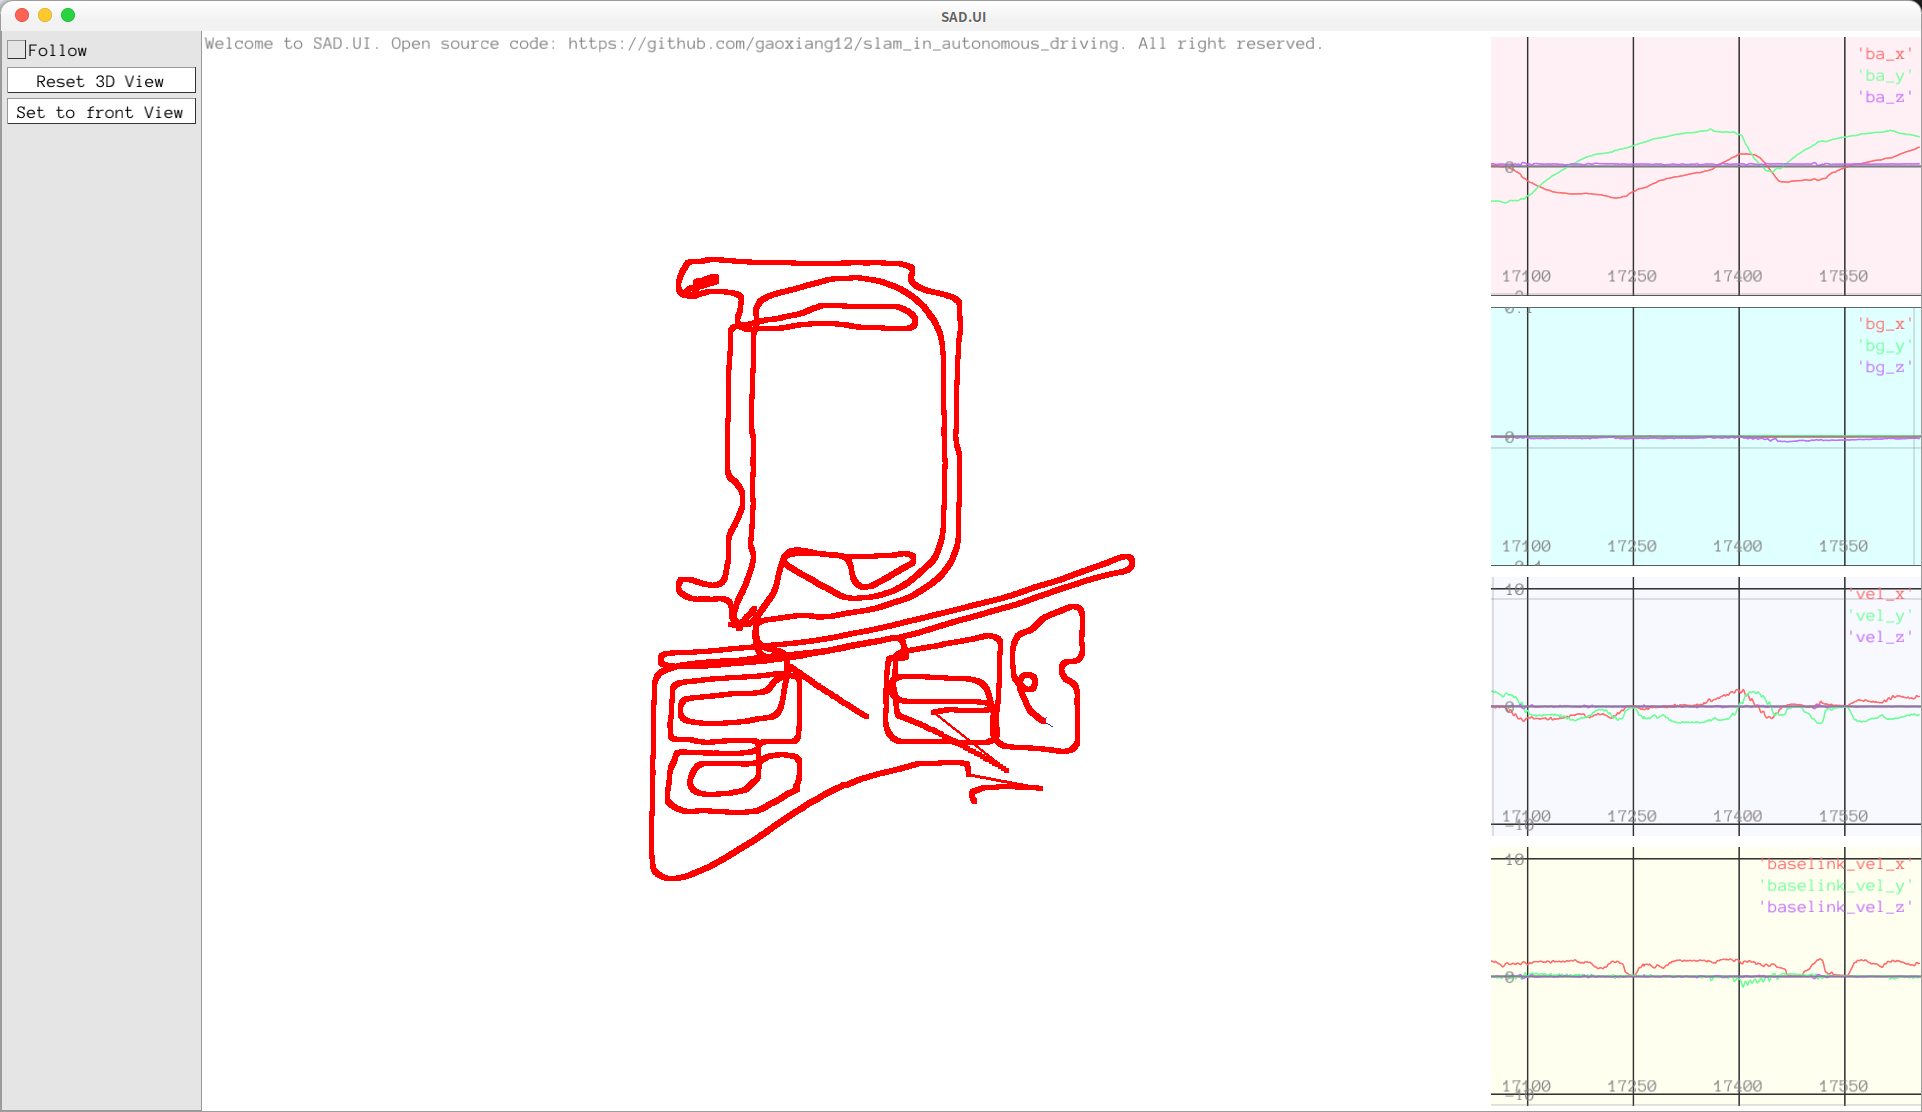
\includegraphics[width=1.0\textwidth]{ins/ch3-eskf-gins-ui.png}
%	\caption{ESKF组合导航的实时结果}
%	\label{fig:ch3-eskf-gins-ui}
%\end{figure}
%
%\begin{figure}
%	\centering
%	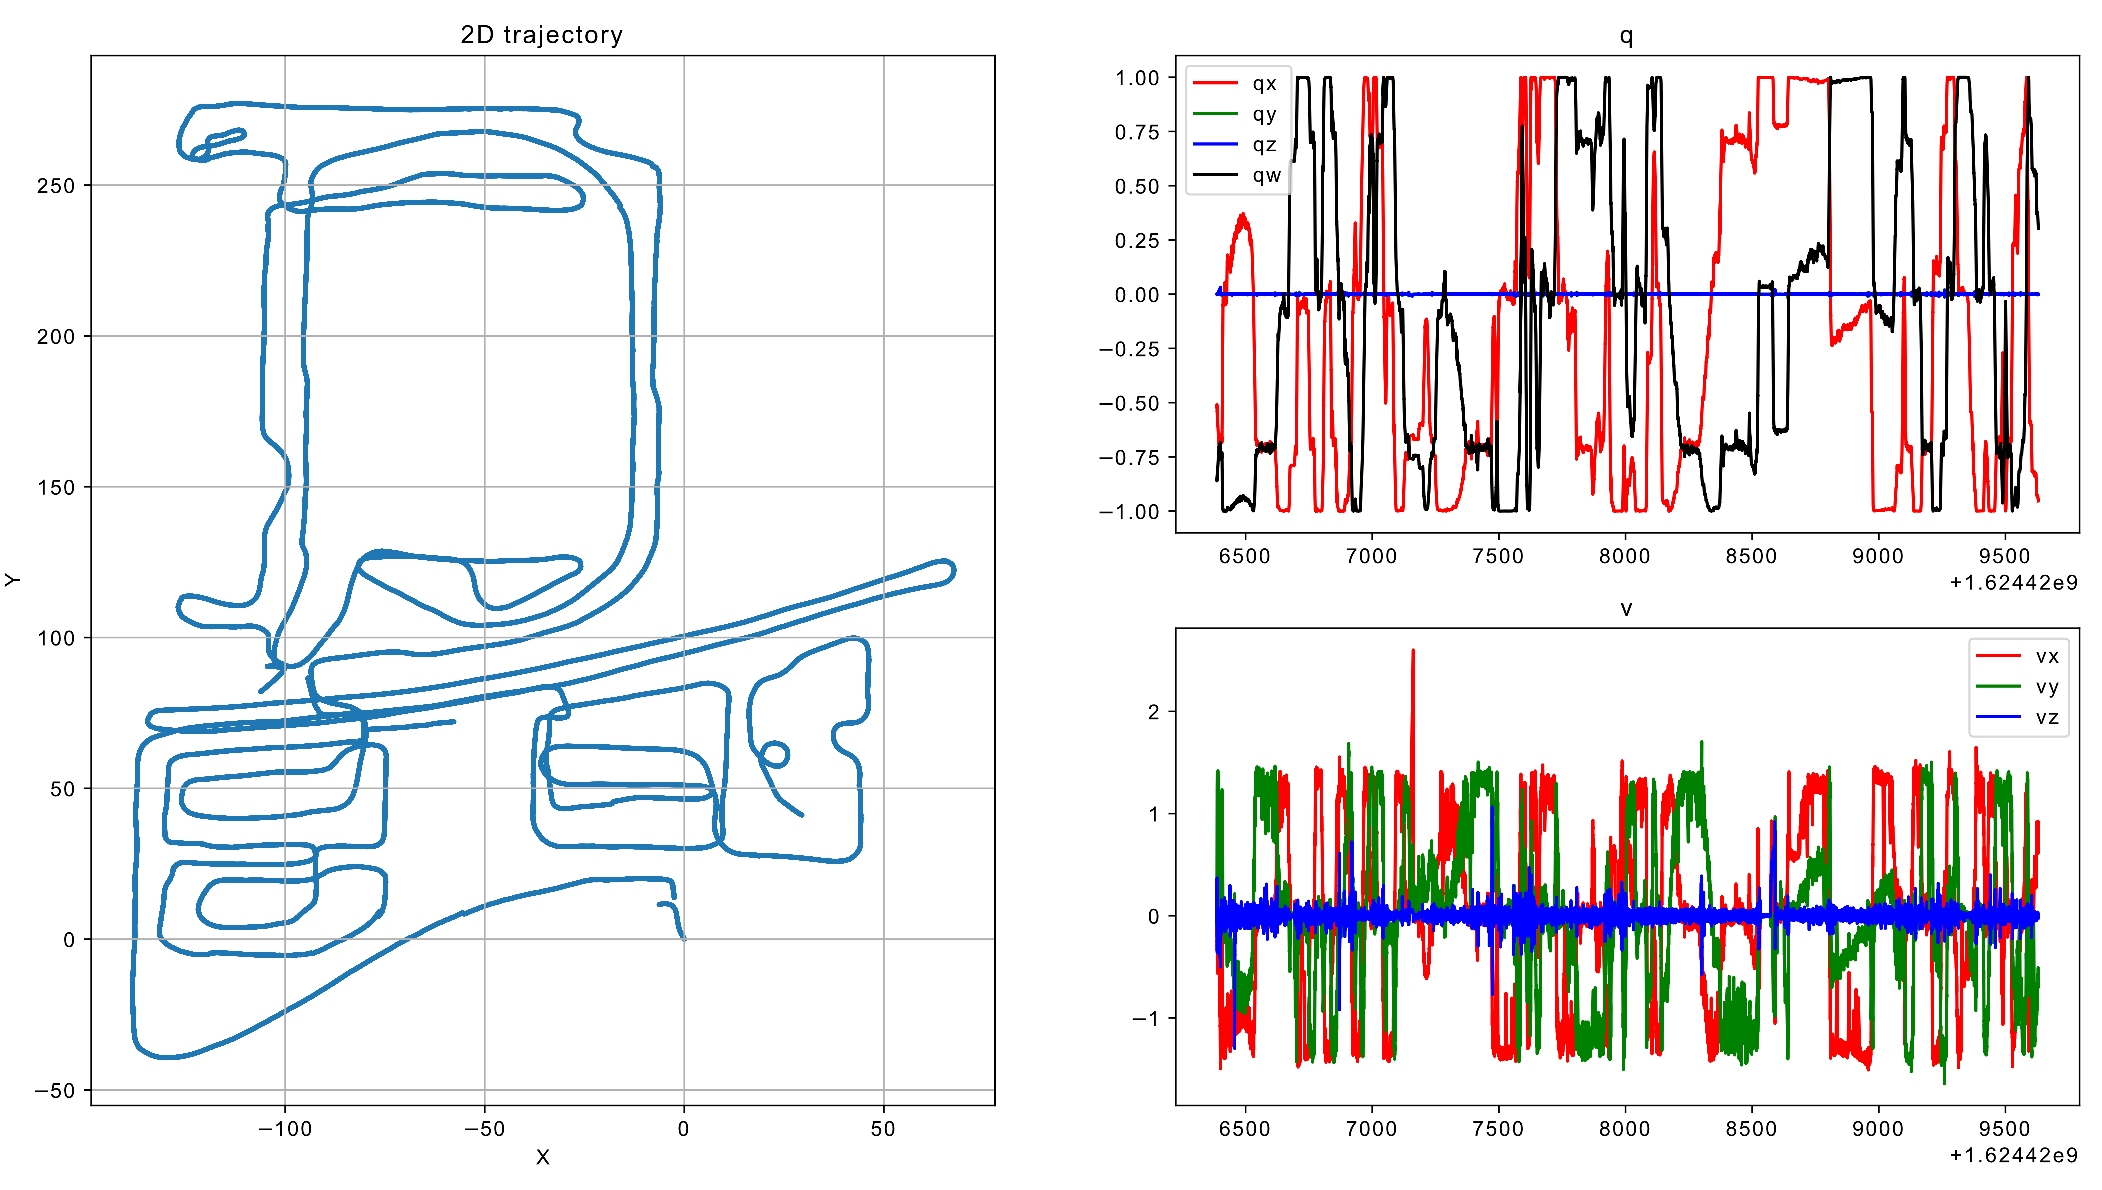
\includegraphics[width=1.0\textwidth]{ins/eskf-traj-out.pdf}
%	\caption{ESKF估计得到的状态变量曲线图。左侧:2D轨迹图,右上:四元数状态;右下:世界系下速度状态;}
%	\label{fig:eskf-traj}
%\end{figure}
%
%对比图~\ref{fig:gnss-traj}~,我们发现它们大体形状是相似的,但个别RTK角度无效的地方,ESKF出现了发散。在实际系统中,如果RTK位置有效而航向无效,我们也可以使用ESKF的角度作为RTK角度,来推算车辆位置。我们把这部分工作留作习题。
%
%现在从实验方面给ESKF下一些评注:
%\begin{enumerate}
%	\item 本节的ESKF展示了如何将IMU观测与GNSS观测进行融合,融合结果整体与GNSS观测相当
%	。如果ESKF能顺利递推,我们也可以将IMU的预测位姿向外输出,得到一个更高频率的定
%	位信号。实际的ESKF也可以融合来自其他观测源的位姿数据。观测方程并不需要有统一的形式,
%	只需要能够进行线性化即可。例如,我们后续会介绍将激光观测源的数据融合至ESKF
%	中。它们的理论基本是一致的,只是观测源的噪声可能有所不同。这种融合的方法称为\textbf{松耦
%	合}。我们也可以将激光点云本身的残差,或者视觉特征点、像素的重投影误差放入观测方程,那
%	就构成了一个\textbf{紧耦合}系统。
%	\item 为了让ESKF保持收敛,我们需要不断地往里加入GNSS的观测信息。如果一段区域内长时间
%	没有GNSS观测,那么IMU递推也将和之前IMU积分一样逐渐\textbf{发散}。可以认为GNSS的观测
%	使得系统的速度、零偏得以固定,或者学术地说,GNSS的观测使这些状态变量\textbf{能观}(observable)
%	了\cite{Vidal-Calleja2007}。我们并不准备严格地讨论一个状态估计器的能观性,虽然那是一个很重要的理论问题。
%	\item 本节我们也没有处理GNSS位姿可能存在的异常值。实际当中的GNSS可能存在无信号,也可
%	能存在报告正常状态,但实际位姿有很大偏离的情况。ESKF的预测——更新模式可以一定程度地
%	平滑IMU和GNSS的位姿,但如果我们不加异常检测,那么异常数据一旦被融入滤波器,很容易带歪整个滤波器,很难再
%	让它返回正确的状态。在ESKF中,我们可以检查\textbf{更新量}(innovation)大小或者预测位置与观测位置之间的距离,来判定是否将这个
%	观测融入滤波器,但这种检查相当依赖于当前时刻的状态估计值,并不好区分\textbf{RTK异常}还是\textbf{滤波器异常}。后面我们向大家介绍的图优化类
%	方法可以更有效地识别并规避GNSS异常值的干扰。
%	\item 接触过图优化的同学可以适当对比ESKF对运动、观测模型的处理方式与图优化具体有何异同
%	。你应该有一种似曾相识的感觉——它们存在非常多的相似之处,但处理方法上也存在一些差异。
%	后面我们会看到,ESKF的更新过程实际是\textbf{边缘化}的过程。它将历史的观测信息边缘化后,
%	变成对当前时刻的一种\textbf{先验}。换句话说,ESKF得到的均值$\bm{x}$和方差$\bm{P}$实际上
%	是下个时刻的先验信息。这个先验信息能够很好地平滑整个滤波器的迭代过程。相应的,通常的图
%	优化方法并没有对整个状态变量的先验,如何处理这个先验信息就成为了算法的关键之处。下一章我们将从图优化角度来重新审视这个问题。
%	相信读者在阅读下一章的内容之后,会对这段描述有更深入的理解。
%\end{enumerate}
%
%
%\subsection{速度观测量}
%我们看到在GINS系统中,如果长时间缺少RTK观测数据,ESKF就变为纯靠IMU积分的递推模式。该模式下位移将很快发散。位移的发散主要原因是缺少速度观测。有没有什么方法可以限制速度的发散呢?最常见的方法是融入车辆的速度传感器。速度测量值主要来自车辆的\textbf{电机转速}或者\textbf{轮式编码器}。大部分轮式机器人会携带一个编码器以测定自身速度,进而推断自身的局部运动情况。有时候我们也可以使用电机转速、油门等底层测量值来测定机器人的速度值。这些速度观测与IMU结合,可以形成局部的\textbf{航迹推算}(Dead Reckoning)。或者,也可以简单地将它们融入ESKF,作为速度的观测量。下面我们来推导它的数学形式和代码实现。
%
%\begin{figure}
%	\centering
%	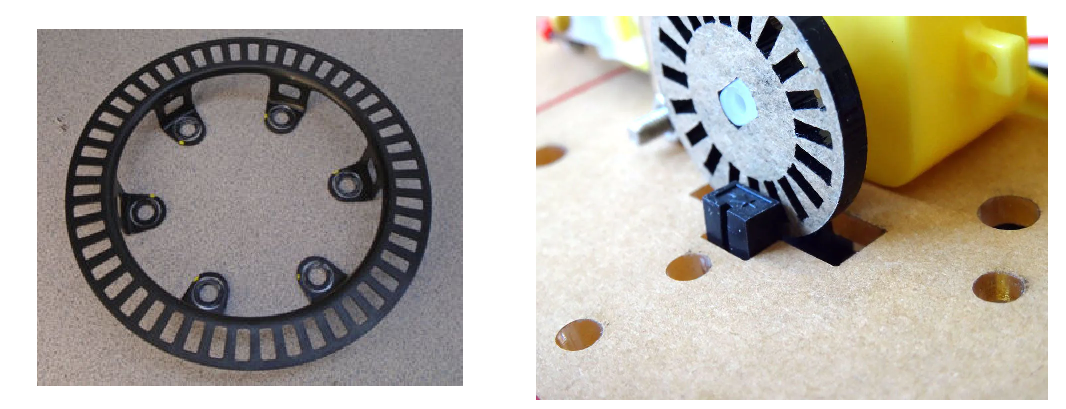
\includegraphics[width=0.7\textwidth]{ins/wheel-speed-encoder.pdf}
%	\caption{一个轮式编码器以及它的安装方式案例}
%	\label{fig:wheel-speed-encoder}
%\end{figure}
%
%图~\ref{fig:wheel-speed-encoder}~展示了一个轮式编码器的案例。这种编码器大多呈圆盘形,边缘有规律的孔洞。在轮子转动时,我们在底盘上安装一个红外或激光的发送接收装置。这个发送接收的结构会穿过轮式编码器上面的孔洞部分。如果轮子转动,接收装置应该有规律地输出信号被阻挡或没有被阻挡两种状态。这种规律的输出反映了轮子转动的距离,结合轮子半径和安装位置信息,也可以进一步反映出车辆相对地面的运动距离。
%
%轮速编码器的特点可以概括如下:
%\begin{enumerate}
%	\item 单个轮式编码器只输出轮子转过的距离,我们可以对这个距离进行采样。如果每隔固定时间采样的话,也可以看成对速度的测量值。
%	\item 如果轮子本身在底盘上的角度是固定不动的,可以通过编码器计算车辆位移。进而,如果使用三轮式的机器人底盘(就像许多扫地机器人和小型机器人一样),还可以通过两侧轮子的位移差异,计算车身的旋转。不过,IMU本身也可以测量车辆的旋转。
%	\item 轮子本身只能测量车辆在\textbf{前进方向}上的速度和位移,但无法测量平行方向或高度方向上的速度和位移。对于一些大型的车辆在颠簸路面上行驶的情况,轮速编码器的结果很可能不符合实际。
%	\item 在实际应用中,轮子很容易受到打滑影响。打滑时,轮子会发生空转,导致编码器虽然有输出,但车辆本身并没有前进的状态。因此,我们可以融入其他状态的观测,得到更好的定位效果。
%\end{enumerate}
%
%本书中,我们将轮速观测作为\textbf{载体系下$X$方向速度}的观测,简而言之,设某两段时间间隔内,我们采样到的轮子转速为标量的$v_{\mathrm{wheel}}$,表示车辆在前进方向上的速度。我们取\textbf{前左上坐标系},即车辆$X$轴向前,$Y$向左,$Z$向上,那么矢量形式的轮速观测可以记为:
%\begin{equation}\label{key}
%\bm{v}_{\mathrm{wheel}} = [v_{\mathrm{wheel}}, 0, 0]^\top.
%\end{equation}
%
%对应的观测模型为:
%\begin{equation}\label{key}
%	\bm{v}_{\mathrm{wheel}} = \bm{R}^\top \bm{v},
%\end{equation}
%其中$\bm{R}, \bm{v}$为车辆当前的状态。于是,轮速可以看成对$\bm{R}^\top \bm{v}$的测量。但实际当中轮速计并\textbf{没有}对$\bm{R}$进行物理意义上的测量,所以更常用的做法是,先根据当前估计的$\bm{R}$,将$\bm{v}_{\mathrm{wheel}}$转到世界坐标系下,直接视为对$\bm{v}$的观测:
%\begin{equation}\label{key}
%	\bm{R} \bm{v}_\mathrm{wheel} = \bm{v}.
%\end{equation}
%
%我们可以把该模型记为抽象的观测模型$\bm{h}(\bm{x})$。显然它对名义状态$\bm{x}$的雅可比矩阵为:
%\begin{equation}\label{key}
%\frac{\partial \bm{h} (\bm{x})}{\partial \bm{x}} = \left[\bm{0}_{3\times 3}, \bm{I}_{3 \times 3}, \bm{0}_{3\times 12} \right].
%\end{equation}
%
%通过雅可比矩阵可也以看出,轮速计并没有对$\bm{v}$以外的状态量有观测效果。如果我们更严格一些,还应该认为$\bm{v}_{\mathrm{wheel}}$没有$Y$, $Z$两个轴上的速度测量。 不过,由于$\bm{v}$受到了观测,加上IMU测量值之后,递推出来的位姿并不会快速发散。轮速的观测函数实现如下:
%
%\begin{lstlisting}[language=c++, caption=src/ch3/eskf.hpp]
%template <typename S>
%bool ESKF<S>::ObserveWheelSpeed(const Odom& odom) {
%	assert(odom.timestamp_ >= current_time_);
%	// odom 修正以及雅可比
%	// 使用三维的轮速观测,H为3x18,大部分为零
%	Eigen::Matrix<S, 3, 18> H = Eigen::Matrix<S, 3, 18>::Zero();
%	H.template block<3, 3>(0, 3) = Mat3T::Identity();
%	
%	// 卡尔曼增益
%	Eigen::Matrix<S, 18, 3> K = cov_ * H.transpose() * (H * cov_ * H.transpose() + odom_noise_).inverse();
%	
%	// velocity obs
%	double velo_l = options_.wheel_radius_ * odom.left_pulse_ / options_.circle_pulse_ * 2 * M_PI / options_.odom_span_;
%	double velo_r =
%		options_.wheel_radius_ * odom.right_pulse_ / options_.circle_pulse_ * 2 * M_PI / options_.odom_span_;
%	double average_vel = 0.5 * (velo_l + velo_r);
%	
%	VecT vel_odom(average_vel, 0.0, 0.0);
%	VecT vel_world = R_ * vel_odom;
%	
%	dx_ = K * (vel_world - v_);
%	
%	// update cov
%	cov_ = (Mat18T::Identity() - K * H) * cov_;
%	
%	UpdateAndReset();
%	return true;
%}
%\end{lstlisting}
%
%在代码实现中,我们能够获取固定时间间隔内左右轮子的转动脉冲数$p$。我们记轮子半径为$r$,每一圈总脉冲为$n$,轮速的测量间隔为$t$,那么速度值$v_{\mathrm{wheel}}$与这几个物理量之间的关系为:
%\begin{equation}\label{key}
%v_{\mathrm{wheel}} = \frac{2 \pi r p}{n t} .
%\end{equation}
%
%在质量模型下,这个速度可以作为车辆线速度的观测值。我们取左右轮的平均值来观测它。当然这是一种粗略的估计,更细致的模型应该考虑到车辆本身的结构和安装参数,但本节主要用来演示它们在ESKF中的作用。我们依然使用轮速计算了误差状态$\delta \bm{x}$,然后合入名义状态中。
%
%要运行带有轮速的ESKF,使用:
%\begin{lstlisting}[language=sh, caption=终端输入:]
%bin/run_eskf_gins --with_odom=true
%\end{lstlisting}
%
%然后按照上一节的方式绘制轨迹结果图。实时UI如图~\ref{fig:ch3-gins-odom}所示。对比图~\ref{fig:ch3-eskf-gins-ui}~可以发现,有几处因为缺少RTK观测而发散的位置明显得到了改善。速度观测对于组合导航是有积极作用的。
%
%\begin{figure}
%	\centering
%	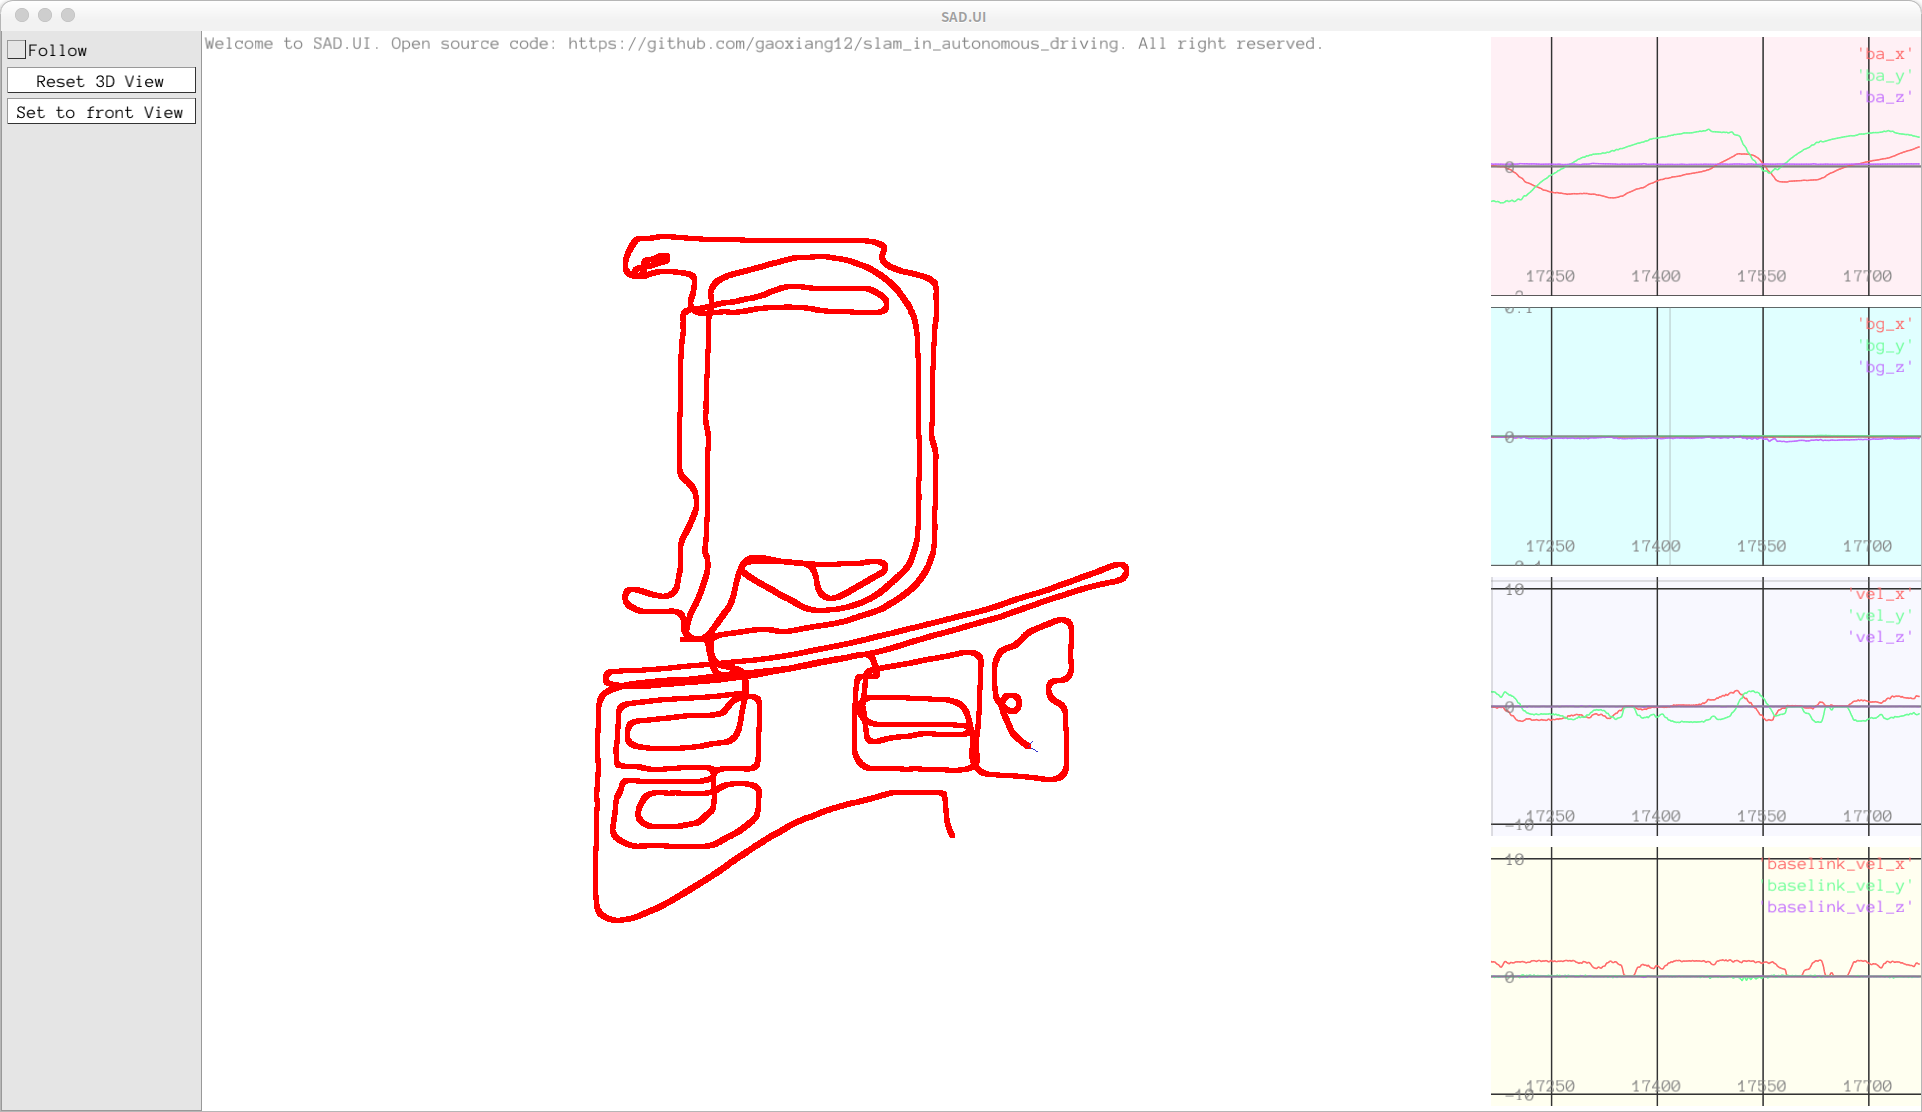
\includegraphics[width=0.7\textwidth]{ins/ch3-gins-odom.png}
%	\caption{添加轮速观测之后的实时轨迹结果}
%	\label{fig:ch3-gins-odom}
%\end{figure}
%
%\section{小结}
%本章介绍了惯性导航系统的基本原理,以误差卡尔曼滤波器形式将IMU、卫星导航和轮速里程计进行了融合,组成了传统的组合导航方案。这种方案在车辆定位方案中是行之有效的。我们通过代码和图形界面演示了它们的工作过程。不过,目前我们还没有引入图像和激光传感器,只能看到车辆的位置和姿态数据,没有直观地描述场景结构。后面的激光章节还将以本节结果为基础,添加2D和3D激光数据,用于建图和定位。
%
%\section*{习题}
%\begin{enumerate}
%\item 证明任意零均值白噪声随机变量乘以任意旋转矩阵作为系数后,仍然是零均值的白噪声,且协
%方差矩阵不变。
%\item 推导以四元数为表示法的ESKF状态转移方程。
%\item 在旋转部分的处理中,使用左乘或右乘的李代数并无本质区别。本书使用了右乘的习惯,请你
%推导以左乘李代数为误差变量的ESKF状态方程。在形式上,左乘是否要比右乘更简单一些?
%\item 如果在ESKF中对运动方程和观测方程稍加改变,很容易得到UKF和IEKF之类的变种。请根据
%本书提供的代码,实现基于UKF或IEKF的组合导航。
%\item 简化ESKF的运动递推过程,不要使用矩阵形式的$\bm{F}$矩阵,而是将各变量的运动过程分别
%列写方程,看看是否有效率提升。有时候这种ESKF也称为\textbf{稀疏的ESKF}。
%\item 尝试简化ESKF中的一些矩阵计算。把没必要计算的部分删掉,仅保留需要的部分,看看有没有
%效率提升。
%\item 对ESKF的更新量进行检查。这个更新量一般为多大?如何来确定异常值判定的阈值?
%\item 设计检查机制,在ESKF中过滤一些RTK的异常观测。
%\item 设计检查机制,让ESKF在长时间没有RTK观测时报告警报信息,并使用最近RTK观测来重置自己。
%\end{enumerate}
